\documentclass[lang=cn, zihao=5]{elegantbook}
\usepackage{hyperref}
\usepackage{booktabs}
\usepackage{float}
\usepackage{svg}

% font settings
\definecolor{mgreen}{RGB}{0,166,82}

% watermark settings
%\usepackage{ctex, draftwatermark, everypage}
%	\SetWatermarkText{DEEP Team 讲义模版}
%	\SetWatermarkLightness{0.95}
%	\SetWatermarkScale{0.3}

% customised commands
\newcommand{\xl}[1]{\overrightarrow{#1}}
\newcommand{\nd}[1]{〔#1〕}
\newcommand{\ssb}[1]{\left( #1 \right)}
\newcommand{\R}{\mathbb{R}}
\newcommand{\C}{\mathbb{C}}
\newcommand{\F}{\mathbb{F}}
\newcommand{\pll}{\kern 0.56em/\kern -0.8em /\kern 0.56em}
\newcommand{\sw}[1]{\boxed{\text{解法 #1}} \ }
\newcommand{\pw}[1]{\boxed{\text{证法 #1}} \ }
\newcommand{\buzhou}[1]{$#1^{\circ} \ $}
\newcommand{\cor}{~\textit{或}~}
\usepackage{ulem}
	\newcommand{\tk}{\uline{\hspace{4em}}}
\newcommand{\pspace}{\vspace{0.5em}}
\usepackage{amsmath,amsfonts}
	\DeclareMathOperator{\spn}{span}
	\DeclareMathOperator{\ic}{i}
	\DeclareMathOperator{\card}{card}
	\DeclareMathOperator{\arccot}{arccot}
	\DeclareMathOperator{\setjianfa}{\textbackslash}
	\DeclareMathOperator{\CRe}{Re}
	\DeclareMathOperator{\CIm}{Im}
	\DeclareMathOperator{\lcm}{lcm}
\newcommand{\examplefont}[1]{\color{mgreen} \textbf{#1}}

\makeatletter
% restore footnote internals to those in normal page, not minipage
\def\tcb@restore@footnote{%
  \def\@mpfn{footnote}%
  \def\thempfn{\arabic{footnote}}%
  \let\@footnotetext\tcb@footnote@collect
}

% collect footnote text
\long\def\tcb@footnote@collect#1{%
  % expand \@thefnmark before appending before app to \tcb@footnote@acc
  \expandafter\gappto\expandafter\tcb@footnote@acc\expandafter{%
    \expandafter\footnotetext\expandafter[\@thefnmark]{#1}%
  }%
}

\def\tcb@footnote@use{%
  \tcb@footnote@acc
  \global\let\tcb@footnote@acc\@empty
}
\global\let\tcb@footnote@acc\@empty


\tcbset{
  % restore for every box
  every box/.style={
    before upper pre=\tcb@restore@footnote
  },
  % use for layer 1 boxes only
  every box on layer 1/.append style={
    after app=\tcb@footnote@use
  }
}
\makeatother

% cover settings

\title{高中数学}

\author{Johnny Tang}
\institute{DEEP Team}
\date{January 21, 2023}

\extrainfo{请:相信时间的力量,敬畏概率的准则}


\cover{cover.png}

% 本文档命令


% 修改标题页的橙色带
\definecolor{customcolor}{RGB}{241,192,184}
\colorlet{coverlinecolor}{customcolor}


\begin{document}

\maketitle

\frontmatter

\mainmatter

\chapter*{写在前面}
\markboth{写在前面}{写在前面}

“例题”主要旨在提升对定理、定义的理解,“练习”则是一些利用既有知识解决的题目.

\tableofcontents

\newpage

\part{预备知识}

\setcounter{chapter}{-1}
\chapter{数理逻辑与集合}

\begin{introduction}
	\item 命题、充分条件、存在与任意
	\item 命题的逻辑运算
	\item 集合、子集与母集
	\item 集合间的运算及其运算律
	\item 区间
\end{introduction}

\section{数理逻辑}

\subsection{命题的概念}

\begin{definition}{命题}
	由一个陈述句表达的、具有真值的判断称为\textbf{命题}.
\end{definition}
\begin{remark}
	有一种特殊的命题,形如“若$p$,则$q$”,这种命题可以帮助我们判断很多要素.
\end{remark}

命题之间有一些特殊关系.

\begin{definition}{充分条件与必要条件} %ayumu数分p1定义0.1
	设命题$A$和$B$.若$A$可以推得$B$,则称命题$A$是$B$的\textbf{充分条件}(sufficient condition),$B$是$A$的\textbf{必要条件}(necessary condition),记作$$A \Rightarrow B,~\text{或}~B \Leftarrow A$$
	若$A$可以推得$B$且$B$可以推得$A$,则称命题$A$和$B$互为\textbf{充分必要条件}(necessary and sufficient condition),简称充要条件,此时也称命题$A$和$B$等价($A$成立当且仅当$B$成立),记作$$A \Leftrightarrow B$$
	此时$B \Rightarrow A$的过程称为充分性,$A \Rightarrow B$的过程称为必要性.
\end{definition}
\begin{remark}
	还有一个类似的逻辑语言:有且仅有(恰有),这意味着存在一个(存在性)且只有一个(唯一性).例如,平面中,过直线外一点有且仅有一条直线与之平行.
\end{remark}
\begin{remark}
	类似于大于等于(小于等于)号,“充分(必要)条件”具有传递性.即“若$A \Rightarrow B$且$B \Rightarrow C$,则$A \Rightarrow C$”.
\end{remark}

可以用图像来更好理解该定义.

\begin{figure}[h!]
	\centering
	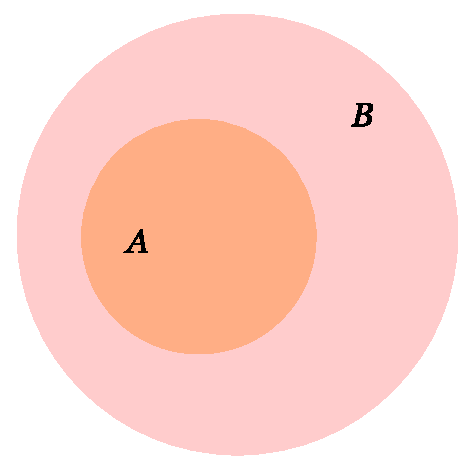
\includegraphics[width=5cm]{attachment/202302191.pdf}
	\caption{例如,此时$A$是$B$的充分且不必要条件}
\end{figure}

\begin{example}
	(1)一个四边形“是菱形”是“它的对角线互相垂直”的\tk 条件. \\
	(2)“$0<x<1$”是“$x<2$”的\tk 条件. \\
	(3)设有命题$p,q$.则“$p \Rightarrow q$”是“$p \Leftrightarrow q$”的\tk 条件. \\
	(4)“$x^2-5x+6 \neq 0$”是“$x \neq 2$”的\tk 条件.
\end{example}
\begin{solution}
	(1)充分且不必要;(2)充分且不必要;(3)必要且不充分;(4)充分且不必要.
\end{solution}

不过这种直观的判断方式比较迷惑,我们可以通过命题的逻辑运算更好地思考这些问题.

\begin{definition}{命题的逻辑运算} %ayumu数分p1定义0.3
	设命题$A$与$B$, \\
	(1)若$A$和$B$中至少有一个命题成立,则称$A$\textbf{或}(or)$B$,记作$$A \vee B$$
	(2)若$A$和$B$同时成立,则称$A$\textbf{且}(and)$B$,记作$$A \wedge B$$
	(3)若$A$的相反形式成立,则称\textbf{非}(not)$A$(或称$A$的否定),记作$$\neg A$$
\end{definition}
\begin{remark}
	关于“且”“或”的否定,存在如下规律:
	$$\neg (A \vee B) = (\neg A) \wedge (\neg B)$$
	$$\neg (A \wedge B) = (\neg A) \vee (\neg B)$$
\end{remark}

另外,对于任意命题的否定,有一个重要法则.在二值逻辑中,该定律实际上告诉我们一个命题$P$要么为真、要么为假.

\begin{proposition}{排中律}
	对于任何命题$P$,$P \vee (\neg P)$为真.
\end{proposition}

\begin{definition}{存在,任意}
	设命题$A$, \\
	(1)若\textbf{存在}(exist)$x$使得命题$A$成立,可以记作$$\exists x~s.t.~A$$
	(2)若对于\textbf{任意}(for all)$x$都能使得命题$A$成立,可以记作$$\forall x,A$$
\end{definition}
\begin{remark}
	“$s.t.$”是“\textit{such that}”的缩写.
\end{remark}
\begin{remark}
	“存在”与“任意”的否定如下:
	$$\neg (\forall x,A) = \exists x~s.t.~\neg A$$
	$$\neg (\exists x~s.t.~A) = \forall x,\neg A$$
\end{remark}

\subsection{特殊的命题}

我们可以对特殊的“若$p$,则$q$”型命题进行更进一步的讨论.

\begin{definition}{原命题,逆命题,否命题,逆否命题}
	设有\textbf{原命题}(primitive proposition)可以表示为$P \Rightarrow Q$的形式. \\
	(1)\textbf{逆命题}(converse proposition)定义为:$$Q \Rightarrow P$$
	(2)\textbf{否命题}(inverse proposition)定义为:$$\neg P \Rightarrow \neg Q$$
	(3)\textbf{逆否命题}(contrapositive proposition)定义为:$$\neg Q \Rightarrow \neg P$$
\end{definition}
\begin{remark}
	此时否命题就是原命题的否定形式,即$\neg (P \Rightarrow Q) = (\neg Q \Rightarrow \neg P)$.
\end{remark}

回顾上一个例题的最后一问,除了用直观的判断方式以外,我们还可以用反证法说明“若$x \neq 2$,则$x^2-5x+6 \neq 0$”.实际上,反证法的本质就是以下命题所述:

\begin{proposition}{逆否命题的真假性}{nifzmkti}
	逆否命题与原命题的真假性相同.
\end{proposition}

这个命题也可用图像来解释:

\begin{figure}[h!]
	\centering
	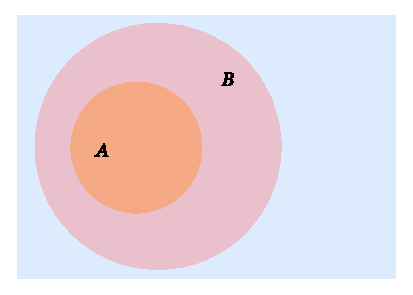
\includegraphics{attachment/202302192.pdf}
	\caption{逆否命题与原命题的真假性比较}
\end{figure}

容易发现,其中“若$A$,则$B$”就等价于“若$\neg B$(即矩形除去大圆的区域),则$\neg A$(即矩形除去小圆的区域)”.




\begin{example}
	证明:$\sqrt{2}$是无理数.
\end{example}
\begin{proof}
	设原命题:“所有能表示为$\dfrac{p}{q}~$($p,q$都是正整数且互质)的形式的数都是有理数”$\Rightarrow$“$\sqrt{2}$是无理数”. \\
	则原命题等价于“所有不能表示为$\dfrac{p}{q}~$($p,q$都是正整数且互质)的形式的数都是无理数”$\Rightarrow$“$\sqrt{2}$是无理数”. \\
	构造逆否命题:“$\sqrt{2}$是有理数”$\Rightarrow$“存在一个不能表示为$\dfrac{p}{q}~$($p,q$都是正整数且互质)的形式的数是有理数”, \\
	由“$\sqrt{2}$是有理数”,设$\sqrt{2}= \dfrac{p}{q}~$($p,q$都是正整数且互质).两边同时平方,有$$2q^2=p^2$$
	这要求$p$是$2$的倍数,因而$p^2$是$4$的倍数,故$q^2$是$2$的倍数.又因为$q$是整数,所以$q$是$2$的倍数,那么$p,q$不互质,即$\sqrt{2}$不能表示为上述形式.这就证明了“存在一个不能表示为$\dfrac{p}{q}~$($p,q$都是正整数且互质)的形式的数是有理数”.由于原命题与逆否命题的真假性相同,故原命题也成立.
\end{proof}

\newpage
\section{集合}

\subsection{集合的概念}

一般地,把一些能够确定的不同的对象看成一个整体,就说这个整体是由这些对象的全体构成的\textbf{集合}(set).其中,构成集合的每一个对象称为\textbf{元素}(element).集合中的元素满足如下性质:确定性,互异性,无序性.特别地,一个集合可以没有元素,这样的集合叫做空集,记作$\varnothing$.

若$x$是集合$X$中的元素,则称$x$\textbf{属于}(belongs to)$X$,记作$x \in X$.反之,$x$\textbf{不属于}$X$记作$x \notin X$.

对于一个集合,我们有两种方式描述集合中的元素:

\begin{enumerate}
	\item 列举法:将集合中的元素一一列举,例如$$\{ 1,2,3,\cdots \}$$其中“$\cdots$”表示类似的元素.
	\item 描述法:为了描述含有无限个元素的集合(即无限集),我们用所含元素的性质来表示该集合,例如$$\kaishu \{ x \in E|P(x) \},~\text{或}\{ x \in E:P(x) \}$$\songti 其中$x$为这些元素的代表元素,$E$是$x$的范围,$P(x)$表示$x$满足的性质.
\end{enumerate}

另外,一些常见的数集有它们特定的表示符号:

\begin{table}[h]
	\centering
	\renewcommand\arraystretch{1.3}
	\begin{tabular}{cc}
		\toprule
		符号           & 数集                    \\
		\midrule
		$\R$         & 实数(real number)集      \\
		$\mathbb{Q}$ & 有理数(rational number)集 \\
		$\mathbb{Z}$ & 整数(integer)集          \\
		$\mathbb{N}$ & 自然数(natural number)集 \\
		\bottomrule
	\end{tabular}
\end{table}

为了描述类似于“正整数集”的集合,我们规定一些标记.例如,$\R ^{+}$(或$\R _{+}$)表示正实数集,$\mathbb{Z}^{-}$表示负整数集,$\mathbb{N}^{*}$表示非零自然数集(等价于正整数集).

以下介绍集合之间的关系:

\begin{definition}{子集和母集}
	设集合$A$和$B$,若$$\forall x,~x \in A \Rightarrow x \in B$$则称$A$\textbf{包含于}(is included in)$B$,或$B$\textbf{包含}(includes)$A$;$A$是$B$的一个\textbf{子集}(subset),$B$是$A$的一个\textbf{母集}(superset),记作$$A \subseteq B,~ \text{或} B \supseteq A$$
	
	当$A$和$B$互为子集时,记作$A=B$.即,$A=B$表示$$\forall x,~ x \in A \Leftrightarrow x \in B$$
	
	特别地,若$$(A \subseteq B) \wedge (A \neq B)$$则称$A$是$B$的一个\textbf{真子集}(proper subset),$B$是$A$的一个\textbf{真母集}(proper superset),记作$$A \subsetneqq B,~ \text{或} B \supsetneqq A$$
\end{definition}
\begin{note}
	上述定义中符号“$\subseteq ,\subsetneqq$”在一些数学课本中也会写作“$\subset$”等.本书均采用上述写法.
\end{note}
\begin{remark}
	(真)包含关系具有传递性,就如同逻辑运算中“充分条件”有传递性一样.
\end{remark}

由上述定义,不难证明,空集是任意集合的子集、是任意非空集合的真子集.

有时我们需要研究某个有限集合的元素个数.设有限集$A$,可以用$\card (A)$表示其元素个数(card即\textit{cardinal},基数).另外,有限集$A$的\textbf{阶}也表示其元素个数,记作$|A|$.

\begin{proposition}{有限集合的子集个数}
	对于一个有限集$A$,它的子集个数为$2^{|A|}$个,真子集个数为$2^{|A|}-1$个.
\end{proposition}
\begin{proof}
	\sw{一}使用“贡献法”.对于给定的一个$A$的子集,任何一个$a_i~(i=1,2,\cdots ,n)$要么在其中,要么不在其中,由乘法原理,这样做就会生成$2^n$个不同的子集.对于一个有限集$A$,其真子集恰会比其子集少一个$A$,即真子集个数为$2^n-1$. \\
	\sw{二}设集合$\{ a_1, \cdots ,a_n \}$.对$n$较小的情况进行子集的枚举:
	\begin{align*}
		n=1&,\quad \varnothing, \{ a_1 \} \\
		n=2&,\quad \color{red} \varnothing, \{ a_1 \},\{ a_2 \},\{ a_1,a_2 \} \color{black} \\
		n=3&,\quad \color{red} \varnothing, \{ a_1 \},\{ a_2 \}\color{black},\{ a_3 \},\color{red} \{a_1,a_2\} \color{black},\{ a_2,a_3 \},\{ a_3,a_1 \},\{ a_1,a_2,a_3 \}
	\end{align*}
	容易发现,每次从$n$增加到$n+1$时,$n$的情况中的子集全部被“继承”到$n+1$的情况里,又将新增加的元素$a_{n+1}$放在每一个继承下来的子集里形成一族新的子集(以$n=2 \to 3$为例,红色部分即为“继承”,黑色部分即为增加).由这种递推关系,可以得到$n$元集合的子集个数为$2^n$. \\
	注:在不使用数学归纳法时,这种证明实际上是不严谨的.
\end{proof}

\subsection{集合间的运算与运算律}

类似于上文对子集和母集的定义,我们可以从集合中元素的角度来研究集合间的运算.

\begin{definition}{集合的交、并、差、补}
	设集合$A$和$B$, \\
	(1)$A$与$B$的\textbf{交集}(intersection),记作$A \cap B$,定义为$$A \cap B := \{ x|(x \in A) \wedge (x \in B) \}$$
	(2)$A$与$B$的\textbf{并集}(union),记作$A \cup B$,定义为$$A \cup B := \{ x|(x \in A) \vee (x \in B) \}$$
	(3)$A$与$B$的\textbf{差集}(difference),记作$A-B$或$A \setjianfa B$,定义为$$A \setjianfa B := \{ x|(x \in A) \wedge (x \notin B) \}$$
	(4)设$U$为\textbf{全集}.$A$的\textbf{补集}(complement),记作$\complement _{U}{A}$,定义为$$\complement _{U}{A} := \{ x|(x \in U) \wedge (x \notin A) \}$$
	若已知该全集(题目中明确定义),$A$的补集也可记作$\overline{A}$.
\end{definition}
\begin{remark}
	“$A := B$”表示用$B$定义$A$.
\end{remark}
\begin{note}
	两集合间的差集并不要求它们有包含关系,而只是从一个集合中“除去”在另一个集合中的元素.
\end{note}

\begin{proposition}
	设集合$A,B$,
	$$A \cap B = B ~ \Leftrightarrow ~ B \subseteq A ,\quad A \cup B = A ~ \Leftrightarrow ~ B \subseteq A$$
\end{proposition}
\begin{proof}
	以第一个为例. \\
	\buzhou{1}充分性:由$B \subseteq A$,有$\forall x, x \in B \Rightarrow x \in A$.于是$$B = \{ x|x \in B \} = \{ x|(x \in B) \wedge (x \in B) \} \subseteq \{ x|(x \in A) \wedge (x \in B) \} = A \cap B$$
	又因为$(A \cap B) \subseteq B$,于是$A \cap B = B$. \\
	\buzhou{2}必要性:由$A \cap B = B$可得$B \subseteq (A \cap B)$.又因为$(A \cap B) \subseteq A$,于是$B \subseteq A$.
\end{proof}

上述定义与命题如果用图像的形式来看,会自然许多:

\begin{center}
	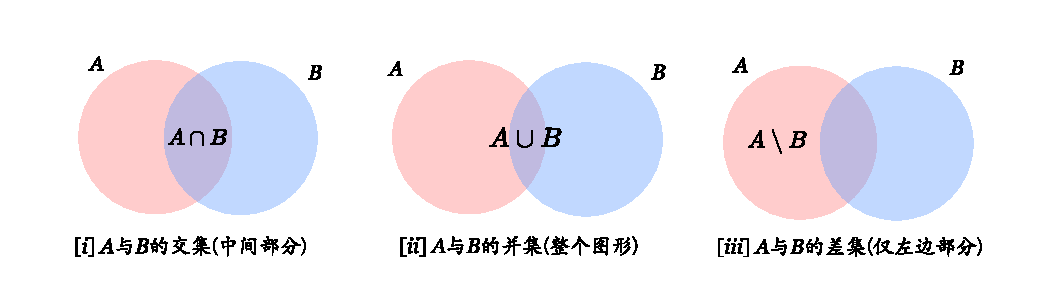
\includegraphics{attachment/20230318jihe.pdf}
\end{center}
\begin{figure}[H]
	\centering
	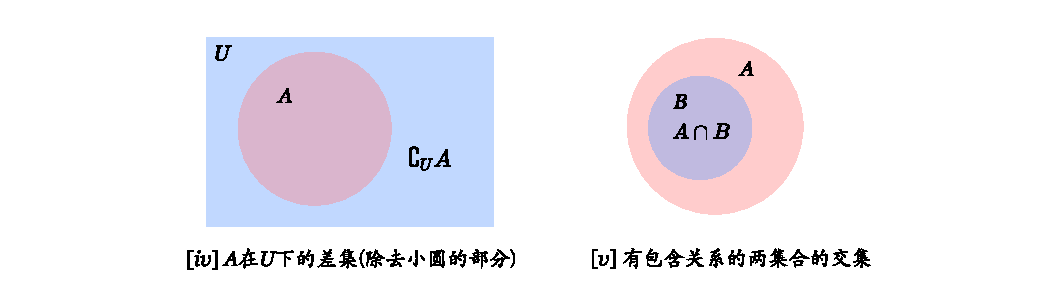
\includegraphics{attachment/20230318jihe2.pdf}
	\caption{集合间的运算图示}
\end{figure}

就像对于加减乘除运算,我们要研究其运算律一样,集合的交、并、补运算也有类似的运算律.

\begin{proposition}{集合运算的运算律}
	设集合$A$和$B$,全集$U$. \\
	(1)它们的交、并运算满足交换律,即$$A \cap B = B \cap A \qquad A \cup B = B \cup A$$
	(2)它们的交、并运算满足结合律,即
	$$A \cap B \cap C = (A \cap B) \cap C = A \cap (B \cap C)$$
	$$A \cup B \cup C = (A \cup B) \cup C = A \cup (B \cup C)$$
	(3)它们的交运算与并运算之间满足分配律,即
	$$(A \cap B) \cup C = (A \cup C) \cap (B \cup C)$$
	$$(A \cup B) \cap C = (A \cap C) \cup (B \cap C)$$
	(4)它们的交、并运算与补运算之间满足摩根律(或称德摩根定理,De Morgan's theorem),即$$\overline{A \cap B} = \overline{A} \cup \overline{B} \qquad \overline{A \cup B} = \overline{A} \cap \overline{B}$$
\end{proposition}

实际上,集合之间的交、并与逻辑运算中的和、或是一样的.例如,不等式$x^2-4x+3 \geq 0$的取值范围为$$\{ x|(x \leq 1) \vee (x \geq 3) \} = \{ x|x \leq 1 \} \cup \{ x|x \geq 3 \}$$

为了更方便地表示上述结果,引入区间的概念:

\begin{definition}{区间}
	定义$\R$上的一种特殊数集为\textbf{区间}(interval).例如 \\
	$$(a,b):=\{ x \in \R | a<x<b \} \quad \textit{“开区间”}$$
	$$[a,b]:=\{ x \in \R | a \leq x \leq b \} \quad \textit{“闭区间”}$$
	$$(a,b]:=\{ x \in \R | a<x \leq b \} \quad \textit{“左开右闭区间”}$$
	$$(-\infty,b):=\{ x \in \R | x<b \}$$
	$$[a,+\infty):=\{ x \in \R | x \geq a \}$$
	$$(-\infty ,+\infty):= \R $$
	其他形式的区间定义相似.
\end{definition}

上文例子中$x$的取值范围就可以表达为$$(-\infty ,1] \cup [3,+\infty )$$

\begin{problemset}
	\item 集合$A=\{ 2,0,1,3 \},~B = \{ x|-x \in A,2-x^2 \notin A \}$,则集合$B$中所有元素的和为\tk .
	\item 由三个实数构成的集合,既能表示为$\{ a,1,b/a \}$,也能表示为$\{ a^2,a+b,0 \}$,则$a^{99}+b^{99}=$\tk .
	\item 已知$A=\{ 2,5 \}$,$B = \{ x|x^2+px+q=0 \}$,且$A \cup B = A$,$A \cap B = \{ 5 \}$,则$pq=$\tk .
	\item 已知$M,N$均为$\mathbb{R}$的子集,且$(\complement _{\mathbb{R}} M) \subseteq N$,则$M \cup (\complement _{\mathbb{R}} N)=$\tk .~(用$M,N$表示)
\end{problemset}
\begin{psolution}
	\item 由题意可知,集合$B=\{ -2,-3 \}$,则$B$中所有元素的和为$-5$.
	\item \sw{一}由于$1$和$0$不能相等,且$a \neq 0$,于是$b/a=0$,即$b=0$.又由$a^2 \neq a,~a^2=1$,可知$a=-1$.综上,$a^{99}+b^{99}=-1$. \\
	\sw{二}由题,$\begin{cases}
		a+1+\dfrac{b}{a} = a^2+(a+b) + 0 \\ a \times 1 \times \dfrac{b}{a} = a^2 \times (a+b) \times 0
	\end{cases}$,由第二个式子可知$b=0$,代回第一个式子,解得$a= \pm 1$,又因为$a^2 \neq a+b$,于是$a=-1$.综上,$a^{99}+b^{99}=-1$.
	\item 由$A \cup B = A$,$A \cap B = \{ 5 \}$,可知$B \subsetneqq A$且$5 \in B$,即$B=\{ 5 \}$.这意味着二次方程$x^2+px+q=0$恰有一个解$x=5$,于是$p=-10,~q=25$,进而$pq=-250$.
	\item 可以作一个换元的操作:令$P=\complement _{\mathbb{R}} M$,则$M=\complement _{\mathbb{R}} P$(也即$P \cup Q=\R ,~P \cap Q = \varnothing$).于是$P \subseteq N$,所求即为$(\complement _{\mathbb{R}} P) \cup (\complement _{\mathbb{R}} N)$.由命题\ref{pro:nifzmkti}可知$(\complement _{\mathbb{R}} N) \subseteq (\complement _{\mathbb{R}} P)$,于是原式等于$\complement _{\mathbb{R}} P$,即为$M$.
\end{psolution}


\chapter{算术预备知识}

\begin{introduction}
	\item 幂运算及其运算律
	\item 对数运算及其运算律
	\item 求和符号的定义与常见求和技巧
\end{introduction}

\section{幂运算与对数运算}

首先介绍\textbf{幂}(power)的概念.对于单项式$a^n(n \in \mathbb{Q})$,令$n=\frac{p}{q}$,
$$a^{\frac{p}{q}}:=\sqrt[q]{a^p} \ (p,q \in \mathbb{Z})$$

这就是有理数次幂的严格定义.其中,$a$称为底数,$n$称为指数,$a^n$的值称为幂值.若$n$是无理数,可以通过计算其相邻的有理数逼近,也可以借助指数函数进行定义(后文会提到).

幂运算的运算律如下:

\begin{proposition}{幂函数的运算律}
	设$a,b,m,n \in \R $. \\
	(1)同底数幂相乘$$a^m \times a^n = a^{m+n}$$
	(2)同指数幂相乘$$a^m \times b^m = (ab)^m$$
	(3)幂的幂$$(a^m)^n=a^{mn}$$
\end{proposition}

接着介绍对数的概念.一般地,若$a^x=y~(a>0,a \neq 1)$,则称$x$为以$a$为底$y$的\textbf{对数}(logarithm),记作$x = \log_{a}{y}$,其中$a$叫做底数,$y$叫做真数(这里人为要求$a>0$是因为当$a\leq 0$时运算不可逆,也即对数函数不单调);读作“以$a$为底$y$的对数”.

通常把以$10$为底的对数叫做\textbf{常用对数}(化学中pH值的计算公式就有利用到它),简记为$\log_{10}{N}=\lg N$;把以自然常数$e$为底的对数叫做\textbf{自然对数},简记为$\log_{e}{N}=\ln N$.

对数运算有两条重要性质:(1)$~\log_{a}{1} = 0,~\log_{a}{a}=1$;(2)$~a^{\log_{a}{N}}=N$.第二条看起来是个废话,但是我们会在下方多次应用.

\begin{example}
	计算:$\log_{2}{8}=$\tk ,~$\log_{\sqrt{5}}{125}=$\tk ,~$\log_{114514}{1}=$\tk ,$\log_{8}{16}=$\tk .
\end{example}
\begin{solution}
	$3$;$6$;$0$;$\dfrac{4}{3}$.
\end{solution}

类似于指数运算,对数运算也有一些重要运算公式:

\begin{proposition}{对数的运算法则}
	假设下列式子都有意义. \\
	(1)加减法$$\log_{\alpha}{MN} = \log_{\alpha}{M} + \log_{\alpha}{N} \qquad \log_{\alpha}{\frac{M}{N}} = \log_{\alpha}{M} - \log_{\alpha}{N}$$
	(2)换底公式$$\log_{\alpha}{x} = \frac{\log_{\beta}{x}}{\log_{\beta}{\alpha}}$$
	(3)指数$$\log_{\alpha ^n}{x^m} = \frac{m}{n} \log_{\alpha}{x}$$
	(4)倒数$$\log_{\alpha}{\beta} = \frac{1}{\log_{\beta}{\alpha}}$$
	(5)链式$$\log_{\alpha}{\beta} \cdot \log_{\beta}{\gamma} = \log_{\alpha}{\gamma}$$
\end{proposition}
\begin{proof}
	这里只选择部分运算法则证明: \\
	(1)加法:由对数的定义,$\alpha ^{\log_{\alpha}{M}} = M,~\alpha ^{\log_{\alpha}{N}} = N$,于是$$MN = \alpha ^{\log_{\alpha}{M}} \cdot \alpha ^{\log_{\alpha}{N}} = \alpha ^{\log_{\alpha}{M} + \log_{\alpha}{N}}$$
	这告诉我们$\log_{\alpha}{MN} = \log_{\alpha}{M} + \log_{\alpha}{N}$. \\
	(2)换底公式:由对数的定义,$\beta ^{\log_{\beta}{x}} = x,~\beta ^{\log_{\beta}{\alpha}} = \alpha$,那么$$x = (\beta ^{\log_{\beta}{\alpha}})^{\frac{\log_{\beta}{x}}{\log_{\beta}{\alpha}}} = \alpha ^{\frac{\log_{\beta}{x}}{\log_{\beta}{\alpha}}}$$
	这告诉我们$\log_{\alpha}{x} = \dfrac{\log_{\beta}{x}}{\log_{\beta}{\alpha}}$. \\
	(5)链式:令$$\log_{\alpha}{\beta} = \frac{\ln{\beta}}{\ln{\alpha}},~ \log_{\beta}{\gamma} = \frac{\ln{\gamma}}{\ln{\beta}}$$
	所以$$\log_{\alpha}{\beta} \cdot \log_{\beta}{\gamma} = \frac{\ln{\beta}}{\ln{\alpha}} \cdot \frac{\ln{\gamma}}{\ln{\beta}} = \frac{\ln{\gamma}}{\ln{\alpha}} = \log_{\alpha}{\gamma}$$
\end{proof}
\begin{remark}
	不难发现,在应用换底公式之后做证明变得很轻松.可以说,如果把“重要性质”比作一个轮子,那么换底公式就是一辆车:用轮子也能向前走(用重要性质也能写证明),但远不及一辆车快速与舒适(引入换底公式会十分便捷).
\end{remark}
\begin{remark}
	换底公式的本质是找到了一个“工具对数”作为中间量化简计算.类似于在应用题中我们倾向于在过程中利用符号$\pi $来计算、只在最后一步将$\pi $化为小数.
\end{remark}
\begin{remark}
	由加减法运算法则,可以一窥常用对数的作用.例如,
	$$\lg{120} = \lg{1.2 \times 10^2} = \lg{1.2}+2$$
	$$\lg{0.012} = \lg{1.2 \times 10^{-2}} = \lg{1.2}-2$$
	若要计算$\lg{120}$与$\lg{0.012}$,只需要知道$\lg{1.2}$的值.于是$\lg{N}$可以被用在换底公式中作为“工具对数”来近似计算.
\end{remark}

\begin{example}
	(1)计算:$5^{\lg 20} \times 0.5^{\lg 0.5}=$\tk ;$6^{\lg 40} \times 5^{\lg 36}=$\tk . \\
	(2)已知$\log_{18}{9}=a,~18^b=5$,则$\log_{36}{45}=$\tk .~(用$a,b$表示) \\
	(3)设$a,b,c$都是正数,且$3^a=4^b=6^c$,则$a,b,c$的关系为\tk .
\end{example}
\begin{solution}
	(1)$$5^{\lg 20} \times 0.5^{\lg 0.5} = 5^{\lg 20} \times 2^{\lg 2} = 5 \times 5^{\lg 2} \times 2^{\lg 2} = 10$$
	$$6^{\lg 40} \times 5^{\lg 36} = 10^{\lg 6 \cdot \lg 40} \times 10^{\lg 5 \cdot \lg 36} = 10^{\lg 6 \cdot (\lg 40 + \lg 25)} = 216$$
	(2)由所给条件,令$a=\frac{\ln{9}}{\ln{18}}=\frac{2\ln{3}}{\ln{2}+2\ln{3}} ,~b=\frac{\ln{5}}{\ln{18}}=\frac{\ln{5}}{\ln{2}+2\ln{3}}$,则$$\ln{2}=\frac{2-2a}{a}\ln{3},~\ln{5}=\frac{2b}{a}\ln{3}$$
	于是
	$$\log_{36}{45} = \frac{\ln{45}}{\ln{36}} = \frac{\ln{5} + 2\ln{3}}{2\ln{2}+2\ln{3}} = \frac{\frac{2b}{a}+2}{\frac{4-4a}{a}+2} = \frac{a+b}{2-a}$$
	(3)记$3^a=4^b=6^c=t$,则$$a=\log_{3}{t},~b=\log_{4}{t},~c=\log_{6}{t}$$
	于是$$\frac{1}{a}=\log_{t}{3},~\frac{1}{b}=\log_{t}{4},~\frac{1}{c}=\log_{t}{6}$$
	故$$\frac{2}{a} + \frac{1}{b} = \log_{t}{9} + \log_{t}{4} = \log_{t}{36} = \frac{2}{c}$$
\end{solution}

\newpage
\section{求和符号}

为了简明地表示一连串式子求和,定义如下求和符号:

\begin{definition}{求和符号}
	对于整数$m \leq n$:$$\sum_{i=m}^{n} x_i := x_m + x_{m+1} + \cdots + x_{n}$$
	更一般地,设性质$P(x)$,$$\sum_{P(x)} x := \textit{所有满足性质$P(x)$的$x$相加}$$
\end{definition}

给出几个求和符号的例子:
$$\sum_{i=1}^{n} i^2 = 1^2 + 2^2 + \cdots + n^2$$
$$\sum_{j=8}^{10} (4j-3) = (4 \times 8-3) + (4 \times 9 - 3) + (4 \times 10 -3)$$
$$\sum_{i=1}^{n} 1 = 1 + 1 + \cdots + 1~~(\textit{共$n$个$1$})$$
$$\sum_{i=1}^{3} \ssb{\sum_{j=1}^{3} a_ib_j} = \sum_{i=1}^{3} \ssb{a_ib_1+a_ib_2+a_ib_3} = a_1b_1+a_1b_2+a_1b_3+a_2b_1+a_2b_2+a_2b_3+a_3b_1+a_3b_2+a_3b_3$$
$$\sum_{1 \leq i < j \leq 4} a_ia_j = a_1a_2 + a_1a_3 + a_1a_4 + a_2a_3 + a_2a_4 + a_3a_4$$
$$\sum_{\textit{$x$是素数且$0< x \leq 10$}} x = 2+3+5+7$$

\begin{example}
	证明下列求和恒等式:\\
	(1)(后半部分为双重求和符号的性质)$$\ssb{\sum_{i=1}^{n}a_i} \ssb{\sum_{i=1}^{n}b_i} = \sum_{i=1}^{n}\sum_{j=1}^{n} a_ib_j = \sum_{i=1}^{n}\sum_{j=1}^{n} a_jb_i$$
	(2)$$\sum_{i=1}^{n}(a_{i+1}-a_i)=a_{n+1}-a_1$$
	(3)$$\sum_{i=1}^{n} (a_{n+i}-a_i) = \sum_{i=1}^n \sum_{j=i}^{n-1+i}(a_{j+1}-a_j)$$
	(4)$$\sum_{1 \leq i < j \leq n}a_ia_j = \sum_{i=1}^{n-1} \ssb{\sum_{j=i+1}^{n} a_ia_j} = \sum_{j=2}^{n} \ssb{\sum_{i=1}^{j-1} a_ia_j}$$
	(5)$$\ssb{\sum_{i=1}^n a_i}^2 = \sum_{i=1}^{n} a_i^2 + 2\sum_{1 \leq i < j \leq n}a_ia_j$$
	(6)$$\sum_{1 \leq i < j \leq n}(a_i-a_j)^2 = n\sum_{i=1}^{n} a_i^2 - \ssb{\sum_{i=1}^{n} a_i}^2$$
\end{example}
\begin{remark}
	双重求和符号可以理解为有先后顺序的求和,即$$\sum_{i=1}^{n}\sum_{j=1}^{n} a_ib_j = \sum_{i=1}^{n} \ssb{\sum_{j=1}^{n} a_ib_j}$$
\end{remark}

\begin{proof}
	(1)前半部分:$$LHS = \sum_{i=1}^{n} \ssb{a_i \sum_{j=1}^{n}b_j} = \sum_{i=1}^{n} \ssb{\sum_{j=1}^{n}a_ib_j} = \sum_{i=1}^{n}\sum_{j=1}^{n} a_ib_j$$
	后半部分:与上式同理可得$$LHS = \sum_{i=1}^{n}\sum_{j=1}^{n} a_jb_i$$
	故有$$\sum_{i=1}^{n}\sum_{j=1}^{n} a_ib_j = \sum_{i=1}^{n}\sum_{j=1}^{n} a_jb_i$$
	(2)$$LHS = (a_2-a_1) + (a_3-a_2) + \cdots + (a_{n+1}-a_n) = a_{n+1}-a_1$$
	(3)对于每个$i=1,\cdots ,n$,类似于(2)的结论,有$$a_{n+i}-a_i = \sum_{j=i}^{n-1+i}(a_{j+1}-a_j)$$
	对$i$进行累加求和,即得$$\sum_{i=1}^{n} (a_{n+i}-a_i) = \sum_{i=1}^n \sum_{j=i}^{n-1+i}(a_{j+1}-a_j)$$
	(4)对于每个$i=1, \cdots ,n-1$,$$\sum_{i<j \leq n} a_ia_j = \sum_{j=i+1}^{n} a_ia_j$$
	对$i$累加求和,即得$$\sum_{1 \leq i < j \leq n}a_ia_j = \sum_{i=1}^{n-1} \ssb{\sum_{j=i+1}^{n} a_ia_j}$$
	由此,前半部分证毕.类似地,对每个$j=2, \cdots ,n$,$$\sum_{1 \leq i<j} a_ia_j = \sum_{i=1}^{j-1} a_ia_j$$
	对$j$累加求和,即得$$\sum_{1 \leq i < j \leq n}a_ia_j = \sum_{j=2}^{n} \ssb{\sum_{i=1}^{j-1} a_ia_j}$$
	后半部分即证毕. \\
	(5)由(1)中结论,$$LHS = \sum_{i=1}^{n}\sum_{j=1}^{n} a_ia_j = \sum_{i=1}^{n} (a_ia_1+a_ia_2 + \cdots + a_ia_n)$$
	对于每个$i=1, \cdots ,n$,将$a_ia_i$、$a_ia_j~(j<i)$和$a_ia_j~(j>i)$分开求和(注意,第二种不存在$i=1$的情况,第三种不存在$i=n$的情况,否则会与第一种的计数重复),则有$$LHS = \sum_{i=1}^{n} a_i^2 + \sum_{i=2}^{n} \ssb{\sum_{j=1}^{i-1} a_ia_j} + \sum_{i=1}^{n-1} \ssb{\sum_{j=i+1}^{n} a_ia_j}$$
	由(4)中结论,即$$LHS = \sum_{i=1}^{n} a_i^2 + 2\sum_{1 \leq i < j \leq n}a_ia_j$$
	(6)对每个满足$1 \leq i < j \leq n$的$(i,j)$,有$$(a_i-a_j)^2 = a_i^2+a_j^2-2a_ia_j$$
	对所有这样的$(i,j)$累加,则
	\begin{equation}
		\sum_{1 \leq i < j \leq n}(a_i-a_j)^2 = \sum_{1 \leq i < j \leq n} (a_i^2+a_j^2-2a_ia_j) = \sum_{1 \leq i < j \leq n}(a_i^2+a_j^2) -2\sum_{1 \leq i < j \leq n} a_ia_j \label{ex1211}
	\end{equation}
	由(5)中结论,
	\begin{equation}
		2\sum_{1 \leq i < j \leq n}a_ia_j = \ssb{\sum_{i=1}^n a_i}^2 - \sum_{i=1}^{n} a_i^2 \label{ex1212}
	\end{equation}
	将式\ref{ex1212}代入式\ref{ex1211},得
	\begin{equation}
		LHS = \sum_{1 \leq i < j \leq n}(a_i^2+a_j^2) + \sum_{i=1}^{n} a_i^2 - \ssb{\sum_{i=1}^n a_i}^2 \label{ex1213}
	\end{equation}
	对每个$i=1, \cdots ,n-1$,有$$\sum_{i < j \leq n} (a_i^2+a_j^2) = \sum_{i < j \leq n}a_i^2 + \sum_{i < j \leq n}a_j^2 = (n-i)a_i^2 + a_{i+1}^2 + \cdots + a_n^2$$
	对$i$累加求和.注意到,对于每个$a_k$,均在$i=k$时出现$n-k$次、在$i=1,\cdots ,k-1$时分别出现$1$次,即共出现$n-1$次,故
	\begin{equation}
		\sum_{1 \leq i < j \leq n}(a_i^2+a_j^2) = \sum_{i=1}^{n} \ssb{(n-1)a_i^2} = (n-1) \sum_{i=1}^{n} a_i^2 \label{ex1214}
	\end{equation}
	将式\ref{ex1214}带入式\ref{ex1213},可得$$LHS = n\sum_{i=1}^{n} a_i^2 - \ssb{\sum_{i=1}^{n} a_i}^2$$
\end{proof}

\chapter{复数与多项式I}

\begin{introduction}
	\item 复数的概念与运算
	\item 多项式的概念与运算
	\item 多项式的根与Vieta定理
\end{introduction}

复数与多项式在初等数学的代数部分非常重要.本章我们先进行大致介绍,进一步的知识放在代数部分讲解.

\section{复数初步}

在介绍复数之前,我们先来看看这个例子:

\begin{figure}[H]
	\centering
	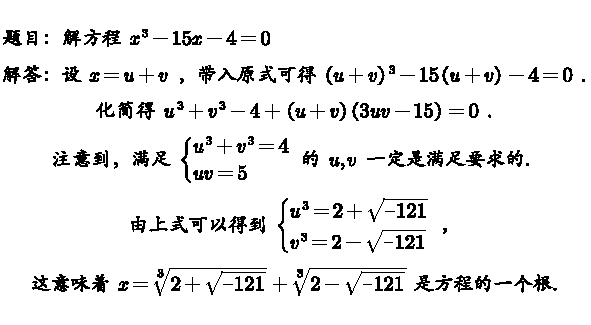
\includegraphics[width=11cm]{attachment/202304152fuuu.pdf}
	\caption{解一个三次方程}
\end{figure}

这种做法看起来“大逆不道”,它居然敢对一个负数开根!但是如果仔细算一算(暂时承认现有的运算律仍存在),由于
$$(2+\sqrt{-1})^3 = 8 + 12\sqrt{-1} - 6 - \sqrt{-1} = 2+11\sqrt{-1}=2+\sqrt{-121}$$
$$(2-\sqrt{-1})^3 = 2-\sqrt{-121}$$
可以得到$x=(2+\sqrt{-1})+(2-\sqrt{-1})=4$.很明显$x=4$的确是原方程的一个根.

就像刚才的例子一样,人们发现有些时候如果允许对负数开根并保持现有运算律不变,最终仍然可以得到正确的计算结果.于是大家开始猜测:这种特殊的由负数开根产生的数真的存在吗?有什么性质?有什么作用?经过长年的猜想与论证,最终构成了数学中的“复数”体系.

\newpage
\begin{definition}{复数,复数间的关系与运算}
	\begin{itemize}
		\item 记$z=a+b\ic ~(a,b \in \R )$为一个\textbf{复数}(complex number),其中$\ic ^2=-1$.定义复数$z$的\textbf{实部}为$a$,\textbf{虚部}为$b$,分别记作$$\CRe (z):=a,\quad \CIm (z):=b$$
		\item 实部为$0$、虚部不为$0$的复数称为纯虚数;虚部为$0$的复数称为实数.
		\item 两个复数相等当且仅当其实部、虚部分别相等,即$$z_1=z_2 ~~ \Leftrightarrow ~~ \CRe (z_1) = \CRe (z_2) ,~ \CIm (z_1) = \CIm (z_2)$$
		\item 由所有复数构成的集合记为$\C$.$\C$上的加法与乘法定义如下:
			$$(a+b\ic ) + (c+d\ic ) = (a+c) + (b+d)\ic $$
			$$(a+b\ic )(c+d\ic ) = (ac-bd) + (ad+bc)\ic $$
	\end{itemize}
\end{definition}
\begin{remark}
	复数之间无法比较大小,只能比较是否相等.
\end{remark}

\begin{proposition}{复数运算的性质}{Fxkvi}
	(1) 交换性质$$\forall \alpha , \beta \in \C , \alpha + \beta = \beta + \alpha , \alpha \beta = \beta \alpha$$
	(2) 结合性质$$\forall \alpha , \beta , \lambda \in \C , (\alpha + \beta) + \lambda = \alpha + (\beta + \lambda) , (\alpha \beta) \lambda = \alpha (\beta \lambda)$$
	(3) 单位元$$\forall \lambda \in \C , \lambda + 0 = \lambda , 1 \lambda = \lambda$$
	(4) 加法逆元$$\forall \alpha \in \C , \exists ! \beta \in \C , \alpha + \beta = 0$$
	(5) 乘法逆元$$\forall \alpha \in \C (\alpha \neq 0) , \exists ! \beta \in \C , \alpha \beta = 1$$
	(6) 分配性质$$\forall \lambda , \alpha , \beta \in \C , \lambda (\alpha + \beta) = \lambda \alpha + \lambda \beta$$
\end{proposition}
\begin{remark}
	“$\exists !$”表示“存在唯一”.
\end{remark}
\begin{proof}
	这里只选择部分性质证明: \\
	(1) 加法交换性质:设$\alpha = a+b\ic , \beta = c+d\ic ~(a,b,c,d \in \R )$,则
	$$\alpha + \beta = (a+b\ic ) + (c+d\ic ) = (a+c) + (b+d)\ic = (c+a) + (d+b)\ic$$
	$$\beta + \alpha = (c+d\ic ) + (a+b\ic ) = (c+a) + (d+b)$$
	因此有$\alpha + \beta = \beta + \alpha$ \\
	(2) 乘法单位元:设$\lambda = a+b\ic ~ (a,b \in \R )$,那么$$1 \lambda = (1+0\ic )(a+b\ic ) = a + b\ic = \lambda$$
	(3) 加法逆元:先证明存在.设$\alpha = a+b\ic $,取$\beta = (-a) + (-b)\ic $,则$\alpha + \beta = 0+0\ic = 0$;\\
	再证明唯一.假设$\beta _1, \beta _2 \in \C $均为$\alpha$的加法逆元,那么$$\beta _1 = \beta _1 + 0 = \beta _1 + \alpha + \beta _2 = 0 + \beta _2 = \beta _2$$
	这与假设矛盾,则$\alpha$的加法逆元是唯一的.
\end{proof}

由此可以引出\textbf{域}的正式定义:

\begin{definition}{域}
	\textbf{域}是一个集合$\F$,它带有加法与乘法两种运算(分别在加法与乘法上封闭),且这些运算满足命题\ref{pro:Fxkvi}所示所有性质.
\end{definition}
\begin{remark}
	最小的域是一个集合$\{ 0,1 \}$,带有通常的加法与乘法运算,但规定$1+1=0$.
\end{remark}

容易验证,$\R$与$\C$都是域.

总是用$\beta$表示$\alpha$的逆元非常不自然,因此定义出加/乘法逆元的表示与减/除法.

\begin{definition}{加法逆元,减法,乘法逆元,除法}
	设$\alpha , \beta \in \C $.
	\begin{itemize}
		\item 令$- \alpha$表示$\alpha$的加法逆元,即$-\alpha$是使得$$\alpha + (-\alpha) = 0$$成立的唯一复数.
		\item 对于$\alpha \neq 0$,令$\alpha ^{-1}$表示$\alpha$的乘法逆元,即$\alpha ^{-1}$是使得$$\alpha (\alpha ^{-1}) = 1$$成立的唯一复数.
		\item 定义$\C $上的\textbf{减法}:$$\beta - \alpha = \beta + (-\alpha)$$
		\item 定义$\C $上的\textbf{除法}:$$\beta / \alpha = \beta (1 / \alpha)$$
	\end{itemize}
\end{definition}

刚才我们用非常严谨的方式研究了复数域上的运算,不过实际上这些运算与实数域上的毫无区别.(因为我们一开始就是希望保持原有运算律不变)

最后,有一个小问题:复数(虚数)的出现是因为在实数域下无法对负数开根,那么复数域会不会有类似的限制以致于产生一些其他的数域呢?

\section{多项式的概念与运算}

\begin{definition}{多项式,多项式的次数}
	\begin{itemize}
		\item 形如$$f(x) = a_nx^n + \cdots + a_1x + a_0~(a_n \neq 0)$$的表达式称为关于$x$的一元$n$次\textbf{多项式}(polynomial).
		\item 当$a_i \in \mathbb{R}~(i=1, \cdots ,n)$时,称其为实系数多项式;当$a_i \in \mathbb{C}~(i=1, \cdots ,n)$时,称其为复系数多项式.一般取$a_i$全为复数的情况来考虑.
		\item 值$n$称为多项式的\textbf{次数}(degree),记作$\deg f(x) = n$.规定恒等于$0$的多项式的次数为$-\infty$.
	\end{itemize}
\end{definition}

\begin{theorem}{多项式间的关系与运算}
	设$f(x) = \sum_{i=0}^{n}a_i x^i,~g(x) = \sum_{i=0}^{m}b_i x^i$.不妨设$m \leq n$,规定$b_i=0~(k > m)$.
	\begin{itemize}
		\item $f(x)=g(x)$的充要条件是$n=m,~a_i=b_i$.
		\item 多项式的加法如下:$$f(x) + g(x) = \sum_{i=0}^{n} (a_i + b_i)x^{i}$$
		\item 多项式的标量乘法如下:$$\lambda f(x) = \sum_{i=0}^{n} (\lambda a_i)x^{i}$$
		\item 多项式的乘法如下:$$f(x) \cdot g(x) = \sum_{i=0}^{n} \sum_{j=0}^{m} a_ib_j x^{i+j} = \sum_{k=0}^{m+n} \ssb{\sum_{i+j=k}a_ib_j}x^k$$
	\end{itemize}
\end{theorem}

类比于整数的带余除法,多项式间也可以有带余除法.

\begin{theorem}{多项式的带余除法}{doxluiiufa}
	若$f(x)$和$g(x)$是两个已知的多项式,其中$g(x)$不是零多项式,那么存在唯一的一对多项式$q(x)$和$r(x)$,使得$$f(x) = g(x) \cdot q(x) + r(x)$$其中$\deg r < \deg g$或$r(x)=0$.称$q(x)$和$r(x)$分别为$f(x)$除以$g(x)$所得的\textbf{商式}与\textbf{余式}.
\end{theorem}
\begin{remark}
	这个定理的证明需要用到数学归纳法,我们会在之后回顾该证明.
\end{remark}

对于已知多项式的带余除法,常常利用“长除法”计算.

\begin{figure}[H]
	\centering
	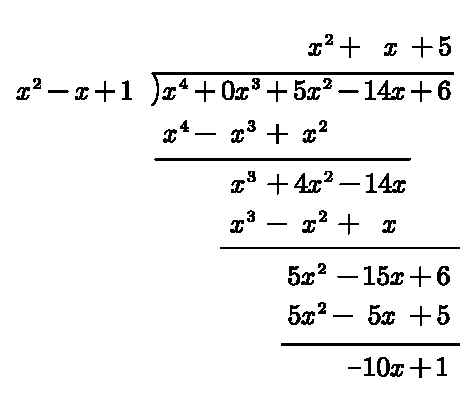
\includegraphics[width=7cm]{attachment/202304151doxlui.pdf}
	\caption{长除法举例}
\end{figure}

在这个例子中,$f(x)=x^4+5x^2-14x+6$,$g(x)=x^2-x+1$,商式$q(x)=x^2+x+5$,余式$r(x)=-10x+1$.

\section{多项式的根与Vieta定理}

\begin{definition}{多项式的根,因式}
	设多项式$f(x)$.
	\begin{itemize}
		\item 若常数$c$满足$f(c)=0$,则称其为$f(x)$的一个\textbf{根}(或\textbf{零点}).
		\item 若多项式$g(x)$满足存在另一个多项式$q(x)$使得$f(x)=g(x) \cdot q(x)$,则称其为$f(x)$的一个\textbf{因式}(factor),亦称$g(x)$\textbf{整除}$f(x)$.
	\end{itemize}
\end{definition}

\begin{theorem}{代数基本定理}
	任何一个非零的一元$n$次复系数多项式,都正好有$n$个复数根.
\end{theorem}
\begin{remark}
	这个定理的证明一般会用到复分析的知识,这里不展开.
\end{remark}

\begin{theorem}{余数定理}{doxluiyuuudkli}
	\begin{itemize}
		\item 多项式$f(x)$除以$x-c$时所得余式等于$f(c)$.
		\item 更一般地,$f(x)$除以$ax-b$时所得余式等于$f(b/a)$.
	\end{itemize}
\end{theorem}
\begin{proof}
	(1)用$f(x)$除以$x-c$,记$f(x)=(x-c)q(x)+r(x)$.由定理\ref{thm:doxluiiufa}可得$\deg r(x) =0$,即$r(x)$是一个常数. \\
	令$x=c$,则$f(c)=r(x)$,即余式$r(x)$的值为$f(c)$. \\
	(2)证明同上,请读者自行验证.
\end{proof}

\begin{theorem}{因式定理}
    对于一个关于$x$的$n$次多项式$$f(x)=a_nx^n+ \cdots +a_1x+a_0$$若存在有理根$c=\dfrac{p}{q}$,则分子$p$是常数项$a_0$的因数,分母$q$是首项系数$a_n$的因数.
\end{theorem}
\begin{proof}
	由定理\ref{thm:doxluiyuuudkli}可得,$f(x)$有根$\dfrac{p}{q}$等价于$f\ssb{\dfrac{p}{q}}=0$,即
	$a_n \ssb{\dfrac{p}{q}}^n + \cdots + a_1 \dfrac{p}{q} + a_0 = 0$,变形得
	$$a_np^n + a_{n-1}p^{n-1}q + \cdots + a_1pq^{n-1} + a_0q^n = 0$$
	两边同时对$q$取模,可得$$a_np^n \equiv 0 \mod q$$
	由于$(p,q)=1$,则$(p^n,q)=1$,于是$a_n \equiv 0 \mod q$,即$q$是$a_n$的因数.同理可得$p$是$a_0$的因数.
\end{proof}

\begin{example}
	(1)分解因式:$2x^4-7x^3+4x^2+2x-1=$\tk ;$x^3-9x^2y+26xy^2-24y^3=$\tk . \\
	(2)多项式$f(x)$除以$2x-3$的余数为$7$,除以$3x+1$的余数为$-4$,则$f(x)$除以$(2x-3)(3x+1)$的余式为\tk . \\
	(3)多项式$f(x)=x^{10}$除以$(x-1)^2$所得的余式为\tk .
\end{example}
\begin{solution}
	(1)第一个:记$f(x)=2x^4-7x^3+4x^2+2x-1$.注意到,$f(1)=0,~f(-1/2)=0$,于是$f(x)$必有因式$(x-1),(2x+1)$. \\
	设$f(x)=(x-1)(2x+1) \cdot q(x)$,由长除法可得$q(x)=x^2-3x+1$,故$$f(x)=(x-1)(2x+1)(x^2-3x+1)$$
	第二个:记$f(x)=x^3-9yx^2+26y^2x-24y^3$为关于$x$的多项式.注意到,$f(2y)=0$,故$f(x)$必有因式$(x-2y)$.同上可得$$f(x)=(x-2y)(x^2-7xy+12y^2)=(x-2y)(x-3y)(x-4y)$$
	(2)记$f(x)=(2x-3)(3x+1) \cdot q(x) + r(x)$.由定理\ref{thm:doxluiiufa}可得$\deg r(x) \leq 1$,记$r(x)=ax+b$. \\
	由余数定理可得$f(3/2)=7,f(-1/3)=-4$.带入上式,有$$\frac{3}{2}a+b=7,\quad -\frac{1}{3}a+b=-4$$
	解得$a=6,b=-2$.则所求余式$r(x)=6x-2$. \\
	(3)记$x^{10}=(x-1)^2 \cdot q(x) + r(x)$.由定理\ref{thm:doxluiiufa}可得$\deg r(x) \leq 1$,记$r(x)=ax+b$,即$$x^{10} = (x-1)^2 \cdot q(x) + ax+b$$
	由余数定理可得$f(1)=0$,即得$a+b=1$.带入上式,有$$x^{10} = (x-1)^2 \cdot q(x) + ax-a+1$$
	作代数变形,得
	$$x^{10}-1 = (x-1)[q(x) \cdot (x-1)+a]$$
	$$(x-1)(x^9+x^8+ \cdots +x+1) = (x-1)[q(x) \cdot (x-1)+a]$$
	于是$x^9+x^8+ \cdots +x+1 = q(x) \cdot (x-1)+a$.在此式中令$x=1$,可得$a=10$. \\
	综上,所求余式为$r(x)=10x-9$.
\end{solution}

关于一元二次方程的Vieta定理我们在初中已经学习过,现在介绍其高阶推广版本.

\begin{theorem}{Vieta定理}
	设多项式$f(x)=a_nx^n + \cdots + a_1x + a_0$有根$x_1, \cdots ,x_n$.则有$$\begin{cases}
		x_1+x_2+ \cdots + x_n=-\dfrac{a_{n-1}}{a_n} \\
		{\displaystyle \sum_{1 \leq i < j \leq n} x_ix_j} = \dfrac{a_{n-2}}{a_n} \\
		\quad \cdots \cdots \\
		{\displaystyle \sum_{1 \leq i_1 < \cdots < i_k \leq n} (x_{i_1} \cdots x_{i_k})} = (-1)^{k} \dfrac{a_{n-k}}{a_n} \\
		\quad \cdots \cdots \\
		x_1 \cdots x_n = (-1)^{n} \dfrac{a_0}{a_n}
	\end{cases}$$
\end{theorem}
\begin{remark}
	Vieta定理适用于$f(x)$为任意系数多项式的情况,因此就算某些根是复数,该定理也成立.
\end{remark}
\begin{proof}
	设$f(x)=a_nx^n + \cdots + a_1x + a_0=a_n(x-x_1)(x-x_2) \cdots (x-x_n)$,将其展开并由多项式相等的定义可得.
\end{proof}

\begin{example}
	(1)三个不同的实数$x,y,z$满足$x^3-3x^2=y^3-3y^2=z^3-3z^2$,则$x+y+z=$\tk . \\
	(2)已知$x_1,x_2,x_3,x_4$是方程$x^4+kx^2+90x-2009=0$的四个根,且$x_1x_2=49$,求$k$的值. \\
	(3)若实数$x_1, \cdots ,x_9$同时满足$$\begin{cases}
		\dfrac{x_1}{11} + \dfrac{x_2}{12} + \cdots + \dfrac{x_9}{19} = 1 \\
		\dfrac{x_1}{21} + \dfrac{x_2}{22} + \cdots + \dfrac{x_9}{29} = 1 \\ 
		\quad \cdots \cdots \\
		\dfrac{x_1}{91} + \dfrac{x_2}{92} + \cdots + \dfrac{x_9}{99} = 1
	\end{cases}$$
	求$x_1+ \cdots + x_9$的值.
\end{example}
\begin{solution}
	(1)记$x^3-3x^2=y^3-3y^2=z^3-3z^2=k$,则$x,y,z$是关于$t$的方程$t^3-3t^2-k=0$的三个不同根.由Vieta定理,$x+y+z=3$. \\
	(2)由Vieta定理,$$x_1+x_2+x_3+x_4=0,\quad x_1x_2x_3+x_1x_2x_4+x_1x_3x_4+x_2x_3x_4=90,\quad x_1x_2x_3x_4=-2009$$
	由于$x_1x_2=49$,有$x_3x_4=-41$,带入前两式可得$$(x_1+x_2)+(x_3+x_4)=0,\quad -41(x_1+x_2)+49(x_3+x_4)=-90$$
	解得$x_1+x_2=1,~x_3+x_4=-1$.由Vieta定理,$$k=x_1x_2+x_1x_3+x_1x_4+x_2x_3+x_2x_4+x_3x_4=8+(x_1+x_2)(x_3+x_4)=7$$
	(3)注意到,$1, \cdots ,9$是关于$t$的方程$$\frac{x_1}{10t+1} + \frac{x_2}{10t+2} + \cdots + \frac{x_9}{10t+9} = 1$$
	的$9$个不同根.将上式整理为$$10^9 \cdot t^{9} + (1 + \cdots + 9 - x_1 - \cdots - x_9) \cdot 10^8 \cdot t^{8} + \cdots = 0$$
	由Vieta定理可得$$1+\cdots +9 = \frac{(x_1 + \cdots + x_9 - 1 - \cdots - 9) \cdot 10^8}{10^9}$$
	化简得$x_1 + \cdots + x_9 = 495$.
\end{solution}

\part{函数与数列}

\chapter{函数}

\begin{introduction}
	\item 映射与函数的概念
	\item 函数的(初等)性质
	\item 常见初等函数
	\item 函数图像的变换
	\item 简单的函数方程
\end{introduction}

\section{映射与函数}

\subsection{映射与函数的概念}

\begin{definition}{映射,函数}
	\begin{itemize}
		\item 设$A$和$B$为两个集合,若对$A$中每个元素$x$,都存在$B$中唯一的元素$y$与之对应,则称此对应关系为一个\textbf{映射}(map),记作$$f:A \to B,~~x \mapsto y$$
		\item $x$在$B$中的对应元素$y$称为$x$在$f$下的\textbf{象}(image),$x$称为$y$在$f$下的\textbf{原象}(preimage),记作$$f(x) = y,~ x \in A$$
		\item 集合$A$称作映射$f$的\textbf{定义域}(domain),记作$D_f$;集合$B$称为映射$f$的\textbf{陪域}(codomain);$A$中所有元素在$f$下的象组成的集合称为$f$的\textbf{值域}(range),记作$R_f$或$f(A)$.
		\item 两个映射相等,当且仅当它们的定义域、对应关系、值域相同.
		\item 定义域与陪域均为数集的映射称作\textbf{函数}(function).
	\end{itemize}
\end{definition}

定义域、陪域与值域的关系如下:

\begin{figure}[h!]
	\centering
	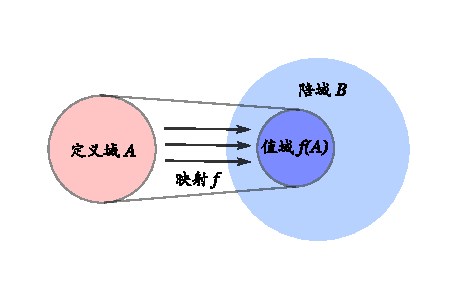
\includegraphics[width=10cm]{attachment/20230403ykue.pdf}
	\caption{定义域、陪域、值域的关系}
\end{figure}

\begin{definition}{特殊的映射}
	设映射$f:A \to B$.
	\begin{itemize}
		\item 若$A$中的每一个$x$的唯一对应$B$中的一个$f(x)$,则称$f$是\textbf{单射}(injection).
		\item 若对于$B$中的每一个元素$y$,总能找到$A$中的一个$x$使得$f(x)=y$,则称$f$是\textbf{满射}(surjection).
		\item 若$f$既是单射,又是满射,则称$f$是\textbf{双射}(bijection)或一一映射.
	\end{itemize}
\end{definition}

单射、满射、双射举例如下:

\begin{figure}[h!]
	\centering
	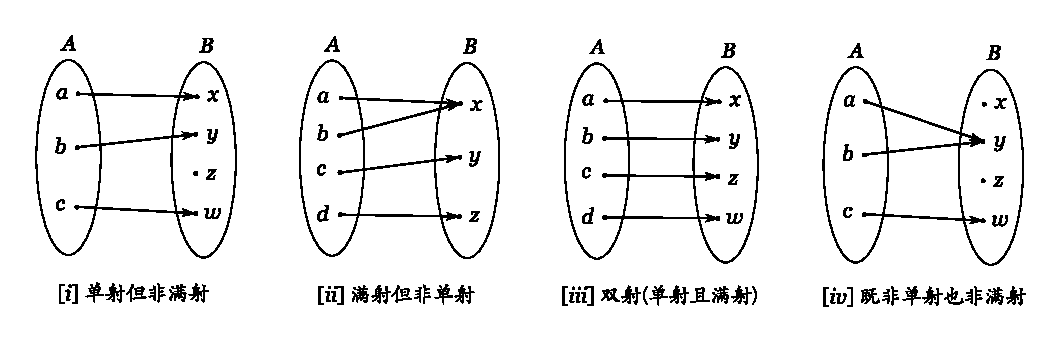
\includegraphics[width=17cm]{attachment/20230403teuuykue.pdf}
	\caption{单射、满射、双射举例}
\end{figure}

利用映射,可以确定集合间元素个数的关系(下列命题其实是另一种理解映射的方法):

\begin{proposition}{集合的对应原理}
	设$A,B$为有限集,$f$为从$A$到$B$的一个映射. 
	\begin{itemize}
		\item 如果$f$为单射,则$|A| \leq |B|$. 
		\item 如果$f$为满射,则$|A| \geq |B|$. 
		\item 如果$f$为双射,则$|A| = |B|$. 
	\end{itemize}
\end{proposition}

刚才我们用了一种静态的方式理解函数.初中介绍的函数概念更为“动态”,即因变量随着自变量的变化而变化的规则称为函数.这种理解方式会在下一小节的例题中体现.

\begin{example}
	(1)判断:下列每组中两个函数是否相同?
	$$f(x)=\frac{x^2-1}{x-1},\quad g(x)=x+1$$
	$$f(x)=x^2,~x \in (-\infty ,0)\cup (0,+\infty),\quad g\ssb{\frac{1}{t}}=\frac{1}{t^2}$$
	(2)构造满足下列条件的映射:定义域和值域分别相同的两个不同映射;双射$f:(0,1) \to (-1,+\infty)$. \\
	(3)设$a \in \R ,~f(x)=\sqrt{x^2+ax+1}$.若$f$的定义域为$\R$,则$a$的取值范围为\tk ;若$f$的值域为$\R ^{+} \cup \{ 0 \}$,则$a$的取值范围为\tk . \\
	(4)已知函数$f(x)=\begin{cases}
		2/x,~x \geq 2 \\ (x-1)^3,~x<2
	\end{cases}$.若关于$x$的方程$f(x)=k$有两个不同的实根,则实数$k$的取值范围为\tk .
\end{example}
\begin{solution}
	(1)第一组:不同.$f$的定义域为$(-\infty ,1)\cup (1,+\infty)$,而$g$的定义域为$\R$. \\
	第二组:相同.$f$和$g$的定义域都是$(-\infty ,0)\cup (0,+\infty)$,对应法则相同,值域都是$\R ^{+}$. \\
	(2)分别构造如下:$$f(x)=x^2, ~g(x)=|x|;\quad f(x)=\frac{1}{x}-2$$
	(3)第一问:即要求对于任意$x \in \R$都有$x^2+ax+1 \geq 0$,只需$\Delta \leq 0$,即得$a \in [-2,2]$. \\
	第二问:即要求对于所有$x \in \R$,$x^2+ax+1$的值取遍$\R ^{+} \cup \{ 0 \}$.由于$$x^2+ax+1 = \ssb{x+\frac{a}{2}}^2 + 1-\frac{a^2}{4}$$
	由二次函数的性质可知$1-\dfrac{a^2}{4} \leq 0$,即得$a \in (-\infty ,-2]\cup [2,+\infty)$. \\
	(4)做出$f(x)$的大致图像如下:
	\begin{figure}[h!]
		\centering
		\includesvg[width=8cm]{gnuplot/202305021edit.svg}
	\end{figure}
	于是得到$k \in (0,1)$.
\end{solution}

\newpage
\subsection{映射与函数的运算}

先介绍一种由定义自然产生的运算:

\begin{definition}{逆映射与反函数} %兴趣一阶I p26
    设映射$f:A \to B$,如果$f$是一个双射,则对任意的$y \in B$,都存在唯一的$x \in A$使得$y=f(x)$.这就产生了一个从$B$到$A$的映射$g$,满足$$x=g(y),~\forall y \in B$$
    该映射称为$f$的\textbf{逆映射}(inverse mapping),记作$$f^{-1}:B \to A$$
    对于这样的逆映射,它的定义域是$B$,值域是$A$.\\
    同样地,设函数$f:A \to B$,如果$f$是一个双射,则$f$的逆映射$f^{-1}$称为函数$f$的\textbf{反函数}(inverse function),其定义域是$B$,值域是$A$.
\end{definition}

不难发现,如果两个函数互为反函数,它们的图像关于$y=x$对称.

函数的加法与标量乘法的定义很符合直觉.

\begin{definition}{函数的加法,标量乘法}
	\begin{itemize}
		\item 对于$f,g:A \to B$,对所有$x \in A$,规定函数的加和$f + g$满足$$(f + g)(x) = f(x) + g(x)$$
		函数$f + g$的定义域为$A$,陪域不定.
		\item 对于$f:A \to B$及$\lambda \in \R$,对所有$x \in A$,规定函数的标量乘法得到的乘积$\lambda f$满足$$(\lambda f)(x) = \lambda f(x)$$
		函数$\lambda f$的定义域为$A$,陪域为$\lambda B$\footnote{我们用常数乘以集合的方式表示将该集合中每个元素均乘以该常数构成的新集合}.
	\end{itemize}
\end{definition}

那么函数之间的乘法该是如何的?实际上,如果单纯地将$f(x)$与$g(x)$的值相乘,得到的新函数很难研究.我们更倾向于研究一种特殊的“乘法”:

\begin{definition}{映射与函数的复合} %兴趣一阶I p26
    设映射$f:A \to B$,$g:B \to C$,则它们的\textbf{复合映射}(composite mapping)~$gf:A \to C$定义为$$(gf)(x)=g(f(x)) \ (x \in A)$$
    注意复合运算有先后顺序.容易说明映射$gf$的定义域为$A$,值域为$C$.\\
    当集合$A,B,C$均为数集时,可以得到类似的复合函数定义.
\end{definition}
\begin{remark}
	为了强调复合运算,$gf$也可记作$g \circ f$.
\end{remark}

容易验证,这样的“乘法”运算满足结合律与分配律、不满足交换律.

有了函数的“乘法”,自然可以得到函数的“乘方”运算.我们一般将$f \circ f \circ \cdots \circ f~(n\textit{次复合})$称作$f$的$n$次迭代,记作$f^n$.

另外,如果定义“恒等映射”$I:A \to A,I(x)=x$为乘法单位元,“零映射”$0:A\to A,0(x)=0$为加法单位元,用类似于复数的方法我们可以定义函数的乘法逆元、加法逆元.注意到,这里的乘法逆元就是逆映射,即$$f^{-1} \circ f (x) = x$$
其余性质读者可参考复数章节证明.

\begin{example}
	(1)求下列函数的反函数:$$f(x)=2x+3,x\in (0,3);\quad y=\frac{6x-5}{x-1};\quad f(x)=x^3-3x^2+9x$$
	(2)已知$f(x+1)=x^2+x$,则$f(x)=$\tk ;已知$f(\sqrt{x})=3x-2\sqrt{x}$,则$f(x)=$\tk . \\
	(3)若函数$y=f(x)$的图像经过点$(2,4)$,则$y=f(20-2x)$的图像必过点\tk . \\
	(4)函数$y=f(x+1)$的反函数是$y=f^{-1}(x+1)$,已知$f(1)=4007$,则$f(1998)=$\tk . \\
\end{example}
\begin{solution}
	(1)第一个:记$y=f(x)$,那么$y \in (3,9)$,$x=\dfrac{y-3}{2}$,于是$$f^{-1}(x)=\frac{x-3}{2},~x \in (3,9)$$
	第二个:由于$y=6+\dfrac{1}{x-1} \in (-\infty ,6)\cup (6,+\infty)$,所以$$f^{-1}(x) = 1+\frac{1}{x-6},~x \in (-\infty ,6)\cup (6,+\infty)$$
	第三个:记$y=f(x)$,注意到$y-27=(x-3)^3 \in \R$,故$$f^{-1}(x) = \sqrt[3]{x-27}+3$$
	(2)第一个:记$t=x+1$,则$f(t)=t(t-1)=t^2-t$,故$f(x)=x^2-x$; \\
	第二个:记$t=\sqrt{x} \geq 0$,则$f(t)=3t^2-2t$,故$f(x)=3x^2-2x,~x \in [0,+\infty )$. \\
	(3)题目条件即$f(2)=4$,令$20-2x=2$,此时$x=9,~y=4$.于是$y=f(20-2x)$的反函数过点$(4,9)$. \\
	(4)由于$y$的反函数为$y=f^{-1}(x+1)$,可知$y+1=f(x)$,将$y=f(x+1)$代入,即得$f(x+1)+1=f(x)$.于是有
	\begin{align*}
		f(1998)-f(1997)&=-1 \\
		f(1997)-f(1996)&=-1 \\
		\cdots \cdots \\
		f(2)-f(1)&=-1
	\end{align*}
	将上式累加可得$f(1998)-f(1)=-1997$,则$f(1998)=4007-1997=2010$.
\end{solution}

\newpage
\section{常见初等函数}

初等函数,是指用基本初等函数进行有限次加减乘除、乘方、开方、复合操作后得到的函数.(注意,不可以进行分段函数操作)

在中学阶段可以遇见的基本初等函数,大致可以分为以下几类:常值函数、指数函数、对数函数、幂函数、三角函数、反三角函数.对于这些函数的概念、图像与性质,我们逐一介绍.(注:三角函数与反三角函数在下一章介绍)

所有的初等函数都是实值函数,即自变量$x$是实数;所有的初等函数都是连续的.(在下一节会用到)

\begin{definition}{常值函数}
    形如$$f(x)=C \ (C \in \mathbb{R}, C\textit{是常数})$$
    的函数称为\textbf{常值函数}(constant function).它的定义域为$\mathbb{R}$,值域为$\{ C \}$.
\end{definition}

\begin{definition}{幂函数}
    形如$$f(x)=x^{\alpha} \ (\alpha \text{是常数})$$
    的函数称为\textbf{幂函数}(power function).
\end{definition}
\begin{remark}
	请注意,当$\alpha =0$时,$f(x)=x^0$并不是常值函数,因为该函数的定义域不包括$0$.
\end{remark}

幂函数的性质不过多介绍.只需知道例如$f(x)=x^3$或$f(x)=\sqrt[4]{x}$的函数都是幂函数.

\begin{definition}{指数函数与对数函数}
	形如$$f(x)=a^x, \ a>0 , a\neq 1$$
    的函数称为\textbf{指数函数}(exponential function).它的定义域为$\mathbb{R}$,值域为$\mathbb{R}^{+}$. \\
    形如$$f(x)=\log_{a}{x}, \ a>0,a \neq 1$$
    的函数称为\textbf{对数函数}(logarithmic function).它的定义域为$\mathbb{R}^{+}$,值域为$\mathbb{R}$.
\end{definition}

指数函数与对数函数的诸多性质都很相似,因为它们互为反函数.

\begin{proposition}{指数函数与对数函数的性质}
    指数函数$f(x)=a^x$具有以下性质:
    \begin{itemize}
        \item 定义域:$\mathbb{R}$
        \item 值域:$\mathbb{R}^+$
        \item 单调性:当$0<a<1$时,为减函数;当$a>1$时,为增函数
        \item 图像:恒过定点$(0,1)$
    \end{itemize}
    对数函数$f(x)=\log_{a}{x}$具有以下性质:
    \begin{itemize}
        \item 定义域:$\mathbb{R}^{+}$
        \item 值域:$\mathbb{R}$
        \item 单调性:当$0<a<1$时,为减函数;当$a>1$时,为增函数
        \item 图像:恒过定点$(1,0)$
    \end{itemize}
    对数函数$f(x)=\log_{a}{x}$与指数函数$f=a^{x}$($a>0$且$a \neq 1$)互为反函数.它们的图像关于$y=x$对称.
\end{proposition}

\begin{figure}[h!]
	\centering
	\includesvg[width=10cm]{gnuplot/202304201edit.svg}
	\caption{指数函数的图像}
\end{figure}

\begin{figure}[h!]
	\centering
	\includesvg[width=6cm]{gnuplot/202304202edit.svg}
	\caption{对数函数的图像}
\end{figure}

顺便说一句,在学习幂运算时,我们无法定义无理数次幂,只能通过实数的连续性逼近.现在我们可以定义$$a^x = \ssb{e ^{\ln a}}^x = e^{x \cdot \ln a}$$
其中$x \in \C$~(是的,甚至可以推广到复数域).这个定义是良定义,因为由指数函数与对数函数复合带来的连续性与我们之前通过实数连续性逼近相吻合.

\begin{example}
	(1)函数$f(x)=\ssb{1/2}^{\sqrt{-x^2-2x+3}}$的值域为\tk . \\
	(2)设$f(x)=\min \{ 2^x,x+2,10-x \}$,则$f(x)$的最大值为\tk . \\
	(3)函数$f(x)=3+2 \cdot 3^{x+1} - 9^x~(-1 \leq x \leq 2)$的最大值为\tk . \\
	(4)若对任意$x \in (-\infty ,-1)$,$(m-m^2) \cdot 4^x + 2^x + 1 >0$恒成立,则实数$m$的取值范围为\tk .
\end{example}
\begin{solution}
	(1)由题可知,$\sqrt{-x^2-2x+3} = \sqrt{-(x+1)^2 + 4} \in [0,2]$.故$f(x)$值域为$[1/4,1]$. \\
	(2)作出$f(x)$的图像如下:
	\begin{figure}[h!]
		\centering
		\includesvg[width=7cm]{gnuplot/202305071edit.svg}
	\end{figure}
	于是可知$f(x)$的最大值为$6$,在$x=4$时取得. \\
	(3)记$t=3^x \in [1/3,9]$,故$$f(x) = -t^2 + 6t + 3$$
	则$f(x)$的最大值为$12$,在$t=3$即$x=1$时取得. \\
	(4)记$t=2^x \in (0,1/2)$,故原不等式等价于$$m-m^2 > -\frac{t+1}{t^2}$$恒成立.记$u=1/t \in (2, \infty)$,则$$-\frac{t+1}{t^2} = -\frac{\frac{1}{u}+1}{\frac{1}{u^2}} = -(u^2+u) < -6$$
	联系上式,恒有$m-m^2 \geq -6$,于是$m \in [-2,3]$.
\end{solution}

\begin{remark}
	这里对“恒成立”与“存在性”问题做一个说明:例如,若对所有$x \in I$都有$f(x) \geq c$~($c$为参数,下同),那么$f(x)$在$I$上的最小值应$\geq c$;若存在$x \in I$使得$f(x) \geq c$,那么$f(x)$在$I$上的最大值应$\geq c$~(否则,若最大值比$c$小,则一定不存在满足条件的$x$).其余的情况可以由此例类推. \\
	本题的(4)问就是恒成立问题.我们先进行代数变形将参数与变量分离,接着求出带变量式子的最大值,使之恒小于等于常数部分. \\
	在解决这类问题时,一定要注意端点值能否取到,最好代回原题进行验证.
\end{remark}

\newpage
有两类特殊的初等函数,在研究最值问题时很常见.

\begin{example}
    设函数$$f(x)=mx+\frac{n}{x}~(m,n>0)$$
    请指出它的定义域、值域并作出示意图.
\end{example}
\begin{solution}
	该函数定义域为$(-\infty ,0) \cup (0,+\infty)$,值域为$(-\infty ,-y_0] \cup [y_0 ,+\infty )$.作图如下:
    \begin{figure}[h!]
		\centering
		\includesvg[width=7cm]{gnuplot/202304221edit.svg}
	\end{figure}
	
	\noindent
	实际上,由均值不等式可得,这里的$y_0$就是$2\sqrt{mn}$,$x_0$就是$\sqrt{n/m}$.
\end{solution}

\begin{example}
    设函数$$f(x)=mx-\frac{n}{x}~(m,n>0)$$
    请指出它的定义域、值域并作出示意图.
\end{example}
\begin{solution}
	该函数定义域为$(-\infty ,0) \cup (0,+\infty)$,值域为$\R$.作图如下:(其中,直接计算可得$x_0=\sqrt{n/m}$.)
    \begin{figure}[h!]
		\centering
		\includesvg[width=7cm]{gnuplot/202304222edit.svg}
	\end{figure}
\end{solution}

\newpage
\section{函数的性质}

\subsection{单调性}

先介绍单调性的概念:

\begin{definition}{函数的单调性} %兴趣一阶I p66
    设函数$f(x)$的定义域为$D$,区间$I \subseteq D$.\\
    若对任意$x_1,x_2 \in I$,且$x_1 < x_2$,有$f(x_1) < f(x_2)$,则称$f(x)$\textbf{单调递增}(monotonically increasing),也称$f(x)$为增函数.\\
    反之,若对任意$x_1,x_2 \in I$,且$x_1 < x_2$,有$f(x_1) > f(x_2)$,则称$f(x)$\textbf{单调递减}(monotonically decreasing),也称$f(x)$为减函数.\\
    如果函数$f(x)$在某个区间$I$上是增函数或减函数,那么就说函数$f(x)$在这个区间上具有\textbf{单调性}(monotonicity).区间$I$叫做$f(x)$的单调区间.
\end{definition}
\begin{remark}
    有些时候,将定义中的条件分别改为$f(x_1) \leq f(x_2)$、$f(x_1) \geq f(x_2)$的函数,也被称为不减函数、不增函数.
\end{remark}
\begin{note}
    要注意描述单调区间的语言:例如,\\
    函数$$f(x)=\frac{1}{x}$$
    在$(- \infty , 0)$\color{red}{和}\color{black}$(0 , + \infty)$上单调递减.它有两个单调区间,而不能看做一整个,这是因为存在例如$f(-1) < f(1)$的情况;\\
    函数$$ f(x)=\begin{cases}
    	x &x<0 \\
    	x+1 &x>0
    \end{cases}$$
    在$(- \infty , 0) \color{red}{\cup}\color{black} (0 , + \infty)$上单调递增.它只有一个单调区间.
\end{note}

注意到,如果一个函数在某个区间上连续且单调,它在这个区间上一定是个单射.(注:所有初等函数都是连续的)

\begin{proposition}{函数单调性的变化规律}
    设函数$f(x),g(x)$,为了方便计算,假定它们的单调区间$I$相同.\\
    (1)函数的加法$f+g$:增函数$+$增函数 $\Rightarrow$ 增函数;减函数$+$减函数 $\Rightarrow$ 减函数.\\
    (2)函数的减法$f-g$:增函数$-$减函数 $\Rightarrow$ 增函数;减函数$-$增函数 $\Rightarrow$ 减函数.\\
    (3)函数的复合$g \circ f$~(当$f$的值域包含于$g$的单调区间时):增函数 $\circ$ 增函数 $\Rightarrow$ 增函数;增函数 $\circ$ 减函数 $\Rightarrow$ 减函数;减函数 $\circ$ 增函数 $\Rightarrow$ 减函数;减函数 $\circ$ 减函数 $\Rightarrow$ 增函数.
\end{proposition}
\begin{proof}
    这里只选择(1)及(3)的部分进行证明,剩下的读者自证不难. \\
    (1)第一部分:任取$x_1,x_2 \in I$使得$x_1 < x_2$.由题知$f(x_1) < f(x_2),~g(x_1) < g(x_2)$.将上两式相加,即得$(f+g)(x_1) < (f+g)(x_2)$.于是$f+g$在$I$上是增函数. \\
    (3)第二部分:任取$x_1,x_2 \in I$使得$x_1 < x_2$.由题知$f(x_1) > f(x_2)$.于是$g(f(x_1)) > g(f(x_2))$,即$(gf)(x_1) > (gf)(x_2)$.于是$gf$在$I$上单调递减.
\end{proof}
\begin{remark}
	注意,以上命题并不能直接作为定理使用,解题时需给出证明.
\end{remark}

\begin{example}
	(1)设函数$f(x)=\log_{1/2}(x^2-2x-3)$,试讨论$f(x)$的单调区间并利用定义证明之. \\
	(2)设函数$$f(x)=\begin{cases}
		(1/3)^x &x \leq 0 \\ (2a-1)x+(1-a) & x>0
	\end{cases}$$在$\R$上是减函数,则$a$的取值范围为\tk .
\end{example}
\begin{solution}
	(1)由$x^2-2x-3 > 0$,可知$f(x)$的定义域为$(-\infty ,-1) \cup (3,+\infty)$. \\
	$f(x)$在$(-\infty ,-1)$单调递增,在$(3,+\infty)$单调递减,下证前者(后者同理可得): \\
	任取$x_1<x_2<-1$,则
	\begin{align*}
		f(x_1)-f(x_2) &= \log_{1/2}(x_1^2-2x_1-3) - \log_{1/2}(x_2^2-2x_2-3) \\
		&= \log_{1/2}\ssb{\frac{x_1^2-2x_1-3}{x_2^2-2x_2-3}}
	\end{align*}
	其中,由于$g(x)=x^2-2x-3$在$(-\infty ,-1)$单调递减且恒为正,知$\dfrac{g(x_1)}{g(x_2)} > 1$.于是$$f(x_1)-f(x_2) < 0$$
	即$f(x)$在$(-\infty ,-1)$单调递增. \\
	(2)若$a=1/2$,则$f(x)$在$\R$上为不增函数,不是严格减函数; \\
	若$a < 1/2$,可知$f(0)=1$,则$1-a \leq 1$,于是$a \in [0,1/2)$. \\
	综上,$a$的取值范围为$[0,1/2)$.
\end{solution}

\begin{theorem}{区间根定理}
    假设函数$f(x)$满足以下条件:
    \begin{enumerate}
        \item 在区间$a \leq x \leq b$上连续;
        \item $f(a) \cdot f(b)<0$.
    \end{enumerate}
    则在区间$a<x<b$上必定存在至少一个$c$,使得$f(c)=0$.\\
    或者说,当一个函数在$x=a$时有$f(x)<0$且在$x=b$时有$f(x)>0$,那么它必然有至少一个零点$c$,其中$a<c<b$.反之亦然.
\end{theorem}
\begin{remark}
	“连续性”是一个高等概念,我们暂时还无法详细了解(于是该定理也无法证明).只需要知道,高中阶段研究的函数(即初等函数)都是连续的.
\end{remark}

\begin{example}
	(1)定义一个函数的\textit{不动点}如下:若存在函数$f(x)$定义域中的$x_0$满足$f(x_0)=x_0$,则称$x_0$是$f(x)$的一个\textit{不动点}.设$f(x)=e^x-2$,证明:$f(x)$在区间$(0,2)$内至少有一个\textit{不动点}. \\
	(2)设方程$x^3-3x^2+1=0$有三根$\omega _1 < \omega _2 < \omega _3$.证明:对任意正整数$n$,有$[\omega _1 ^n + \omega _2 ^n] = 0$.(这里,$[x]$表示不超过$x$的最大整数)
\end{example}
\begin{solution}
	(1)即证明$\varphi (x) = e^x-2-x$在$(0,2)$内至少有一个零点. \\
	实际上,由于$\varphi (0) = -1 < 0,~\varphi (2)=e^2-4 > 0$,由区间根定理,这是显然的. \\
	(2)记$f(x)=x^3-3x^2+1$.先对三根做初步估计:注意到,$$f(-1)=-3<0,\quad f(0)=1>0,\quad f(1)=-1<0,\quad f(2)=-3<0,\quad f(3)=1>0$$
	于是$\omega _1 \in (-1,0),~\omega _2 \in (0,1),~\omega _3 \in (2,3)$.进一步地,注意到$$f(-0.5)=0.125>0,\quad f(0.5)=0.375>0,\quad f(-0.6)=-0.296<0,\quad f(0.6)=0.136>0,\quad f(0.7)=-0.127$$
	于是$\omega _1 \in (-0.6,-0.5),~\omega _2 \in (0.6,0.7)$. \\
	当$n=1$时,$\omega _1 + \omega _2 \in (0,0.2)$,则$[\omega _1 + \omega _2]=0$. \\
	当$n=2$时,$\omega _1^2 + \omega _2^2 \in (0.61,0.85)$,则$[\omega _1^2 + \omega _2^2]=0$. \\
	当$n$为奇数且$n \geq 3$时,由于$\omega _2 > -\omega _1$,可知$$\omega _2^n > -\omega _1^n$$
	即$\omega _1 ^n + \omega _2 ^n >0$;另一方面,$\omega _2^n < 0.7^n$,$\omega _1 ^n < -0.5^n$,故$$\omega _1 ^n + \omega _2 ^n < 0.7^n - 0.5^n <1$$
	于是$[\omega _1 ^n + \omega _2 ^n] = 0$. \\
	当$n$为偶数且$n \geq 4$时,显然有$$\omega _1 ^n + \omega _2 ^n >0$$
	另一方面,$\omega _2^n < 0.7^n$,$\omega _1 ^n < 0.6^n$,故$$\omega _1 ^n + \omega _2 ^n < 0.7^n + 0.6^n < 0.7^2 + 0.6^2 = 0.85 < 1$$
	于是$[\omega _1 ^n + \omega _2 ^n] = 0$.
\end{solution}

\newpage
\subsection{奇偶性与对称性}

先介绍奇偶性的概念:

\begin{definition}{奇偶性} %兴趣一阶I p66
    设函数$f(x)$,其定义域$D$关于原点对称.\\
    若对任意$x \in D$,$f(x)=-f(-x)$,则称$f(x)$为\textbf{奇函数}(odd function).\\
    反之,若对任意$x \in D$,$f(x)=f(-x)$,则称$f(x)$为\textbf{偶函数}(even function).\\
    显然,奇函数的图像沿原点中心对称,偶函数的图像沿$y$轴轴对称.
\end{definition}

\begin{proposition}{函数奇偶性的变化规律}
    设函数$f(x),g(x)$,为了方便计算,假定它们的定义域$D$相同.\\
    (1)同奇偶性函数的加减法$f \pm g$:奇函数$\pm$奇函数 $\Rightarrow$ 奇函数;偶函数$\pm$偶函数 $\Rightarrow$ 偶函数.\\
    (2)函数的(代数意义上的)乘法$f(x) \cdot g(x)$:奇函数$\cdot$奇函数 $\Rightarrow$ 偶函数;偶函数$\cdot$偶函数 $\Rightarrow$ 偶函数;奇函数$\cdot$偶函数 $\Rightarrow$ 奇函数.\\
    (3)函数的(代数意义上的)除法:$\frac{1}{\text{奇函数}}$ $\Rightarrow$ 奇函数;$\frac{1}{\text{偶函数}}$ $\Rightarrow$ 偶函数.可以通过函数的(代数意义上的)乘法推广到任意两函数相除.\\
    (4)函数的复合$g \circ f$:奇函数 $\circ$ 奇函数 $\Rightarrow$ 奇函数;奇函数 $\circ$ 偶函数 $\Rightarrow$ 偶函数;偶函数 $\circ$ 奇函数 $\Rightarrow$ 偶函数;偶函数 $\circ$ 偶函数 $\Rightarrow$ 偶函数.
\end{proposition}
\begin{remark}
	如果把复合看做乘法,那么可以把“增减”看做“正负”,“奇偶”看做“奇偶”
\end{remark}
\begin{proof}
    只选择(2)(3)(4)的部分证明: \\
    (2)设奇函数$f(x)$与偶函数$g(x)$,函数$h(x):=f(x) \cdot g(x)$.对任意$x \in D$,有$f(x)=-f(-x),~g(x)=g(-x)$,于是有$$f(x) \cdot g(x) = - f(-x) \cdot g(-x)$$
    即$h(x)=-h(-x)$.又因为$h(x)$的定义域关于原点对称,故$h(x)$是奇函数. \\
    (3)设奇函数$f(x)$,$h(x):=\frac{1}{f(x)}$,其中$h(x)$的定义域是$f(x)$的定义域中除去所有使得$f(x)=0$的$x$,故$h(x)$定义域关于原点对称. \\
    又由于对任意$x \in D$,有$f(x)=-f(-x)$,故$h(x)=-h(-x)$,于是$h(x)$是奇函数. \\
    (4)设奇函数$f(x)$,偶函数$g(x)$,则对任意$x \in D$,有$f(x)=-f(x)$且$g(x)=g(-x)$,于是$$(gf)(-x) = g(f(-x)) = g(-f(x)) = g(f(x)) = (gf)(x)$$
    又因为$(gf)(x)$的定义域关于原点对称,故$gf(x)$为偶函数.
\end{proof}

\begin{example}
	(1)判断下列函数是否具有奇偶性:$$y = \frac{2^x-1}{2^x+1},\quad y=\frac{\sqrt{9-x^2}}{|x+4|+|x-3|},\quad y=\ln \ssb{x + \sqrt{x^2+1}}$$
	(2)设函数$f(x)=\dfrac{x}{(2x+1)(x-a)}$为奇函数,则$a=$\tk . \\
	(3)设函数$f(x)=x^3+x$,当$0 \leq t \leq 1$时,$f(mt)+f(1-m)>0$恒成立,则实数$m$的取值范围为\tk . \\
	(4)设函数$f(x)=\dfrac{(x+1)^2+\sqrt[3]{x}}{x^2+1}$的最大值为$M$,最小值为$m$,则$M+m=$\tk .
\end{example}
\begin{solution}
	(1)第一个:记$f(x)=y$.由于$$f(-x) = \frac{\frac{1}{2^x} -1}{\frac{1}{2^x} +1} = \frac{1-2^x}{1+2^x} = -f(x)$$
	又$f(x)$定义域关于原点对称,故$f(x)$为奇函数. \\
	第二个:记$f(x)=y$.由$9-x^2 \geq 0$知$x \in [-3,3]$,此时$|x+4|+|x-3|=x+4+3-x=7$.于是$$f(-x)=\frac{\sqrt{9-x^2}}{7}=f(x)$$
	又$f(x)$定义域关于原点对称,故$f(x)$为偶函数. \\
	第三个:记$f(x)=y$.由$x + \sqrt{x^2+1} > 0$,可知$x \in \R$.由于$$f(-x) = \ln \ssb{-x+\sqrt{x^2+1}} = \ln \ssb{\frac{1}{x+\sqrt{x^2+1}}} = -\ln \ssb{x + \sqrt{x^2+1}} = -f(x)$$
	又$f(x)$定义域关于原点对称,故$f(x)$为奇函数. \\
	(2)显然,$f(x)$定义域为$\R \setjianfa \{-1/2,a \}$.为使该定义域关于原点对称,令$a=1/2$.代回验证,发现$$f(-x) = \frac{-2x}{(1-2x)(2x+1)} = -f(x)$$
	故$a=1/2$符合题意. \\
	(3)注意到,$f(x)$是奇函数且在$\R$上单调递增,则原不等式等价于$f(mt)>f(m-1)$,即$mt>m-1$在$t \in [0,1]$时恒成立.于是$$m < \frac{1}{1-t}$$
	而右式恒$\geq 1$,则$m \in (-\infty ,1)$. \\
	(4)注意到,$f(x)=1+\dfrac{2x+\sqrt[3]{x}}{x^2+1}$,即$g(x)=f(x)-1$为奇函数,即$f(x)$关于$(0,1)$中心对称,则$M+m=2$.
\end{solution}

\begin{example}
	(1)定义在$\R$上的函数$f(x)$满足$$\forall x,y \in \R ,~f(x+y)+f(x-y)=2f(x)f(y)$$且$f(0) \neq 0$,判断$f(x)$的奇偶性. \\
	(2)证明:任何一个定义域关于原点对称的函数都可以表示为一个奇函数与一个偶函数的和.
\end{example}
\begin{solution}
	(1)令$x=y=0$,则$$f(0)+f(0)=2f(0)f(0) \quad i.e. \quad f(0)\ssb{2f(0)-2}=0$$
	由于$f(0) \neq 0$,可得$f(0)=1$. \\
	令$x=0$,则$$f(y)+f(-y)=2f(0)f(y)$$
	即$f(y)=f(-y)$.又$f(x)$定义域关于原点对称,故$f(x)$为偶函数. \\
	(2)设该函数为$f(x)$,分解为$f(x)=g(x)+h(x)$,其中$g(x)$为偶函数,$h(x)$为奇函数.于是$$f(-x)=g(-x)+h(-x)=g(x)-h(x),\quad f(x)=g(x)+h(x)$$
	可得$$g(x)=\frac{f(x)+f(-x)}{2},\quad h(x)=\frac{f(x)-f(-x)}{2}$$
	经检验,对任意$f(x)$,该构造符合要求.
\end{solution}

对称性其实就是奇偶性在部分区间上的推广.因此,它在定义域上比较自由.

\begin{definition}{对称性} %兴趣一阶I p76
    设函数$f(x)$的定义域为$D$,区间$I \subseteq D$.\\
    函数$f(x)$的图像关于直线$x=a$\textbf{轴对称}当且仅当
    $$ \forall x \in I,~ f(a+x)=f(a-x) $$
    函数$f(x)$的图像关于点$(a,b)$\textbf{中心对称}当且仅当
    $$ \forall x \in I,~ f(a+x)+f(a-x)=2b $$
\end{definition}

可以用图像来理解这一定义:

\begin{figure}[h!]
	\centering
	\includesvg[width=6cm]{gnuplot/202305201edit.svg}
	\caption{中心对称性质的图像}
\end{figure}

以中心对称为例,由图像可知$f(a+x)=b+y,~f(a-x)=b-y$,则$f(a+x)+f(a-x)=2b$.

\begin{proposition}{函数的对称变换}
    设函数$f(x)$与$g(x)$.假设其定义域满足下方自然要求.\\
    (1)$f(x)$与$g(x)$的图像关于直线$x=a$对称,等价于$$\forall x,~f(a+x)=g(a-x)$$
    (2)$f(x)$与$g(x)$的图像关于直线$y=b$对称,等价于$$\forall x,~b+f(x)=b-g(x)$$
    (3)$f(x)$与$g(x)$的图像关于点$(a,b)$对称,等价于$$\forall x,~b+f(a+x)=b-g(a-x)$$
\end{proposition}

\begin{example}
	(1)若函数$y=f(x+2)$是偶函数,则$y=f(16-x)$的对称轴是\tk . \\
	(2)指出下列函数的对称中心:$$y=x^3+3x^2+6x+3,\quad y=\frac{2017^x}{2017^x-1}$$
	(3)若函数$f(x)=(1-x^2)(x^2+ax+b)$的图像关于直线$x=-2$对称,则$f(x)$的最大值为\tk .
\end{example}
\begin{solution}
	(1)由题,$f(x)$关于$x=2$轴对称.那么$f(16-x)$关于$16-x=2$轴对称,即$y=f(16-x)$关于$x=14$轴对称. \\
	(2)第一个:注意到,$f(x)=y=(x+1)^3+3(x+1)-1$.则$y=f(x-1)+1$是奇函数,那么$f(x)$关于$(-1,-1)$中心对称. \\
	第二个:取几个特殊点:$f(1)=2017/2016,~f(-1)=-1/2016$,于是考虑取$f(-x)$看看:$$f(-x)=\frac{\frac{1}{2017^x}}{\frac{1}{2017^x}-1} = \frac{-1}{2017^x-1} = 1-f(x)$$
	故$f(x)$关于$(0,1/2)$中心对称. \\
	(3)由于$f(-1)=f(1)=0$,且$f(x)$关于$x=-2$对称,故$f(-3)=f(-5)=0$,即$$f(x)=-(x+1)(x-1)(x+3)(x+5) = -(x^2+4x-5)(x^2+4x+3) = -(x^2+4x-1)^2+16$$
	其中,$x^2+4x-1 = (x+2)^2-5 \geq -5$,于是$f(x) \leq 16$.
\end{solution}

\newpage
\subsection{周期性}

\begin{definition}{周期性} %兴趣一阶I p76
    设函数$f(x)$的定义域为$D$.\\
    当$f(x)$满足$$\forall x \in D, \exists \ T \in \mathbb{R}, f(x)=f(x+T)$$
    称这样的$T$为函数$f(x)$的\textbf{周期}(period),称$f(x)$为\textbf{周期函数}(periodic function).当$f(x)$有一个最小的正数$T$作为周期,这样的$T$称作最小正周期.
\end{definition}
\begin{remark}
    一个周期函数不一定有最小正周期,例如函数$f(x)=1$.
\end{remark}
\begin{remark}
    当一个函数$f(x)$同时有周期$T_1,T_2$,则$aT_1+bT_2(a,b \in \mathbb{Z})$也为它的周期.更进一步,由Bezout定理,$(T_1,T_2)$也为它的周期.
\end{remark}

\begin{example}
	(1)设定义在$\R$上的函数$f(x)$满足$f(x) \cdot f(x+2)=13$,若$f(1)=2$,则$f(111)=$\tk . \\
	(2)设$f(x)$是$\R$上的奇函数且$f(x+3)=-f(x)$,而当$0 \leq x \leq 3/2$时,$f(x)=x$,则$f(2003)=$\tk . \\
	(3)已知函数$f(x)$满足$f(x)=f(398-x)=f(2158-x)=f(3214-x)$,则$f(0),f(1),\cdots ,f(999)$中最多有\tk 个不同的值.
\end{example}
\begin{solution}
	(1)由于$f(x) \cdot f(x+2)=13$,$f(x+2) \cdot f(x+4)=13$,故$f(x)=f(x+4)$.那么$f(111)=f(3)=13/f(1)=13/2$. \\
	(2)由题给条件,$f(x+6)=-f(x+3)=f(x)$,故$f(2003)=f(-1)=-f(1)=-1$. \\
	(3)将$398-x$视作整体,那么$f(x)$有周期$1760$,同理有周期$1056$,则$f(x)$有周期$(1760,1056)=(704,1056)=(704,352)=352$,那么$f(x)$的最小正周期$T_0 \leq 352$. \\
	于是$\{ f(0),\cdots ,f(999) \} = \{ f(0),\cdots ,f(351) \}$. \\
	又由$f(x)=f(398-x)=f(46-x)$,即$f(x)$关于$x=23$与$x=199$轴对称,可知$\{ f(0),\cdots ,f(351) \} = \{ f(23),\cdots ,f(199) \}$.故最多有$177$个不同的值.
\end{solution}

\newpage
\section{函数的图像}

本节我们着重研究一个问题:如何做出一个函数的大致图像?

首先介绍一些函数图像的变换方式.

\begin{proposition}{绝对值对函数图像的影响}
    设函数$f(x)$,以下解析式不一定是函数.\\
    (1)当$y=f(|x|)$,即将$f(x)$的图像在$y$轴右侧部分沿$y$轴对称,作为在$y$轴左侧的图像.\\
    (2)当$y=|f(x)|$,即将$f(x)$的图像在$x$轴下方部分沿$x$轴翻折.\\
    (3)当$|y|=f(x)$,即将$f(x)$的图像在$x$轴上方部分沿$x$轴对称,作为在$x$轴下方的图像.
\end{proposition}

\begin{remark}
	同样可以得到,\\ 
    (4)当$|y|=|f(x)|$,即将(2)中得到的图像按(3)的法则变换.\\
    (5)当$y=|f(|x|)|$,即将(2)中得到的图像按(1)的法则变换.\\
    (6)当$|y|=|f(|x|)|$,即将(5)中得到图像按(3)的法则变换.
\end{remark}

\begin{proposition}{函数图像的拉伸}
    设函数$f(x)$.\\
    (1)当$y=Af(x)$,即将$f(x)$的图像沿竖直方向拉伸$A$倍.\\
    (2)当$y=f(\omega x)$,即将$f(x)$的图像沿水平方向拉伸$1/\omega$倍.
\end{proposition}

\begin{proposition}{函数的平移变换}
    设函数$f(x)$,变换后的函数为$g(x)$.假设其定义域满足下方自然要求.\\
    (1)$f(x)$的图像向上或向下平移$m$个单位,等价于$$g(x)=f(x)+m \ \text{或} \ g(x)=f(x)-m$$
    (2)$f(x)$的图像向左或向右平移$n$个单位,等价于$$g(x)=f(x+n) \ \text{或} \ g(x)=f(x-n)$$
\end{proposition}

\begin{example}
	作出以下函数大致图像:$$y=\frac{x^2}{1-2|x|},\quad y=\frac{1+2^{x/2}}{1-2^{x/2}},\quad y=\ln \ssb{\frac{1+2^x}{1-2^x}},\quad y=e^x-\ln x$$
\end{example}
\begin{solution}
	(1)先看$f(x)=\dfrac{x^2}{1-2x}$的图像.由于$$f(x)=-\frac{1}{2}x+\frac{1/8}{1/2 - x} - \frac{1}{4} = \frac{1}{2} \ssb{-x+\frac{1/4}{1/2-x}} - \frac{1}{4} = \frac{1}{2} \ssb{(1/2-x)+\frac{1/4}{1/2-x}-1}$$
	故$f(x)$的图像可由$$g(x)=-\ssb{x+\dfrac{1}{4x}}$$
	的图像先向右平移$\dfrac{1}{2}$,再向下平移$1$,最后沿竖直方向拉伸为原来的$\dfrac{1}{2}$得到. \\
	接着取$f(|x|)$,即沿$y$轴左右对称即可.
	\begin{figure}[H]
		\centering
		\includesvg[width=8cm]{gnuplot/202305241edit.svg}
	\end{figure}
	
	\noindent
	(2)先看最基本的$f(x)=\dfrac{1+2^x}{1-2^x}$.容易证明,该函数定义域是$\R \setjianfa \{ 0 \}$,是一个奇函数且单调递增,那么只需考虑$\R ^+$的一侧图像.注意到,在$x \to 0^+$时,$f(x) \to -\infty$;在$x \to +\infty$时,$f(x) \to -1$. \\
	最后取$f(x/2)$,即沿水平方向拉伸为原来的$2$倍得到.
	\begin{figure}[H]
		\centering
		\includesvg[width=8cm]{gnuplot/202305242edit.svg}
	\end{figure}
	
	\noindent
	(3)沿用(2)中最初始的$f(x)$,可知$g(x)=\ln f(x)$的定义域为$\R ^-$.容易证明,$g(x)$单调递增.且在$x \to -\infty$时,$g(x) \to 0$;$x \to 0^-$时,$g(x) \to +\infty$.
	\begin{figure}[H]
		\centering
		\includesvg[width=8cm]{gnuplot/202305243edit.svg}
	\end{figure}
	
	\noindent
	(4)显然$f(x)=e^x-\ln x$的定义域为$\R ^+$.注意到,在$x$比较小时,$e^x$增长缓慢且靠近$1$;在$x$比较大时,$\ln x$增长缓慢且为正.故在$x$较小时图像类似于$y=\ln x+1$,$x$较大时图像类似于$e^x$,但会低一点.
	\begin{figure}[H]
		\centering
		\includesvg[width=8cm]{gnuplot/202305244edit.svg}
	\end{figure}
\end{solution}

\newpage
\section{函数方程略讲}

函数方程,是指这样一类特殊的方程,它的解是某一个函数表达式.解函数方程的技巧有很多,这里无法一一叙述,只好割爱,简要介绍一些基本方法,并将其作为函数章节的复习.完整的方法与例题可以参考\textit{Pang-Cheng, Wu}所著的\textit{Functional Equation}\footnote{https://cdn.bc-pf.org/resources/math/algebra/fe/Pang\_Cheng\_Wu-FE.pdf} .

解决函数方程的基本方法有:赋值法,换元法,柯西法,利用函数的性质等.我们逐一介绍.

\begin{example}{\examplefont{赋值与解方程组}}
	(1)求所有函数$f:\R \to \R$,满足$$\forall x \in \R ,~2f(x)+xf(1-x)=x^3-2$$
	(2)求所有函数$f:\R \to \R$,满足$$\forall x,y \in \R,~f(x-y)=f(x)+f(y)-2xy$$
	(3)求所有函数$f:\mathbb{N} \to \mathbb{N}$,满足$$\forall x,y \in \mathbb{N},~f(x+y)=f(x)+f(y)+3(x+y)\sqrt[3]{f(x)f(y)}$$
\end{example}
\begin{solution}
	(1)令$P(x)$表示$2f(x)+xf(1-x)=x^3-2$. \\
	分别取$P(x)$及$P(1-x)$,有$$\begin{cases}
		2f(x)+xf(1-x)=x^3-2 \\
		2f(1-x)+(1-x)f(x)=(1-x)^3-2
	\end{cases}$$
	将$f(x)$与$f(1-x)$视作变量,将$x$视作参数,联立解得$f(x)=x^2-1$.代回$P(x)$验证,成立. \\
	(2)令$P(x,y)$表示$f(x-y)=f(x)+f(y)-2xy$. \\
	取$P(0,0)$,有$f(0)=f(0)+f(0)$,则$f(0)=0$;取$P(x,x)$,有$2f(x)-2x^2=f(0)=0$,则$f(x)=x^2$.代回$P(x,y)$验证,成立. \\
	(3)根据$P(x,y)$的形式,猜测$f(x)=x^3$,取$g(x):=\sqrt[3]{f(x)}$,下证$g(x)=x$. \\
	$P(x,y)$即为$(g(x+y))^3=(g(x))^3+(g(y))^3+3(x+y)g(x)g(y)$.分别取$P(x,-x),P(x,x),P(2x,-x)$,可得$$\begin{cases}
		(g(0))^3 = (g(x))^3 + (g(-x))^3 \\
		(g(2x))^3 = 2(g(x))^3 + 6x(g(x))^2 \\
		(g(x))^3 = (g(2x))^3 + (g(-x))^3 + 3xg(2x)g(-x)
	\end{cases}$$
	将$g(x),g(-x),g(2x)$视作变量,将$x$视作参数.解得$g(x)=x$.
\end{solution}

\begin{proposition}{Cauchy方程}
	若函数$f$满足$$\forall x,y \in D_f,~f(x+y)=f(x)+f(y)$$
	则称$f$是\textbf{加性的}(additive). \\
	对于加性函数$f$,若其定义域为$\mathbb{Q}$,则有$f(x)=f(1)x$;若其定义域为$\R$,且满足下列三个条件
	\begin{itemize}
		\item $f$在定义域上单调
		\item $f$在定义域上连续
		\item $f$在定义域上有界
	\end{itemize}
	之一,则有$f(x)=f(1)x$,反之则不一定.
\end{proposition}
\begin{proof}
	第$1$步~下证
	\begin{equation}
		\forall n \in \mathbb{Z},~ f(n)=nf(1) \label{prop_cauchy1}
	\end{equation}
	首先,取$P(0,0)$,得$f(0+0)=f(0)+f(0)$,于是有$f(0)=0$. \\
	其次,由$$f(n)=f(n-1)+f(1)=f(n-2)+2f(1)=\cdots =f(0)+nf(1)$$
	有$\forall n \in \mathbb{Z}^+,~ f(n)=nf(1)$. \\
	最后,取$P(x,-x)$,有$f(0)=f(x)+f(-x)$,则$\forall n \mathbb{Z}^-,~f(n)=-f(-n)=nf(1)$. \\
	综上,式\ref{prop_cauchy1}成立. \\
	第$2$步~下证
	\begin{equation}
		\forall p \in \mathbb{Z},q \in \mathbb{N}^+,~ f\ssb{\frac{p}{q}}=\frac{p}{q} f(1) \label{prop_cauchy2}
	\end{equation}
	首先,由$f$是加性的,显然有$f(x_1+ \cdots +x_n)=f(x_1) + \cdots + f(x_n)$.注意到$$qf\ssb{\frac{p}{q}} = \underbrace{f\ssb{\frac{p}{q}} + f\ssb{\frac{p}{q}} + \cdots + f\ssb{\frac{p}{q}}}_{q~ \rm times} = f\ssb{q \cdot \frac{p}{q}} = f(p)$$
	结合式\ref{prop_cauchy1},立得式\ref{prop_cauchy2}成立. \\
	至此,原命题的前半部分证明完毕.为证明在$\R$上的加性函数是正比例函数的条件,需要用到一些高等工具,这里暂时跳过.
\end{proof}
\begin{remark}
	像这样先证明$\mathbb{Z}$,再证明$\mathbb{Q}$,最后证明$\R$的方法称作Cauchy方法.
\end{remark}

\begin{example}{\examplefont{Cauchy方程}}
	(1)求所有连续函数$f:\R \to \R$,满足$$\forall x,y\in \R,~f(x+y)=f(x)f(y)$$
	(2)求所有函数$f:\mathbb{Q} \to \R$,满足$f(1)=2$且$$\forall x,y \in \mathbb{Q},~f(xy)=f(x)f(y)-f(x+y)+1$$
\end{example}
\begin{solution}
	(1)在$P(x,y)$中,想让等式两侧同取自然对数,故先讨论$f(x)$的值域. \\
	首先注意到,取$P(x,x)$,有$f(2x)=(f(x))^2 \geq 0$. \\
	若存在$a$使得$f(a)=0$,则$\forall x \in \R,~f(x+a)=f(x)f(a)=0$,即此时$f(x)=0$. \\
	若$f(x)$值域不包含$0$,则将$P(x,y)$两侧同取自然对数,可得$$\forall x,y \in \R,~ \ln f(x+y) = \ln f(x) + \ln f(y)$$
	显然$g(x):= \ln f(x)$也是连续的.由Cauchy方程,$g(x)=g(1)x$,则$\ln f(x) = x \ln f(1)$,得$f(x)=(f(1))^x$. \\
	综上,若存在$a$使得$f(a)=0$,则$f(x)=0$;若$f(x)$值域不包含$0$,则$f(x)=(f(1))^x$. \\
	(2)根据$P(x,y)$形式,猜测$f(x)=x+1$.以下分两步给出证明: \\
	第$1$步~下证
	\begin{equation}
		\forall n \in \mathbb{Z},~ f(n)=n+1 \label{ex35221}
	\end{equation}
	取$P(x,1)$,则有$$f(x)=f(x)f(1)-f(x+1)+1$$
	即$f(x+1)=f(x)+1$.对于正整数$n$,有$$f(n)=f(n-1)+1=\cdots = f(1)+n-1=n+1$$
	另一方面,取$P(-x,1)$,则有$$f(-x)=f(-x)f(1)-f(1-x)+1$$
	即$f(-x)=f(1-x)-1$.对于正整数$n$,有$$f(-n)=f(1-n)-1=\cdots = f(0)-n=1-n$$
	综上,式\ref{ex35221}成立. \\
	第$2$步~下证
	\begin{equation}
		\forall p \in \mathbb{Z},q \in \mathbb{N}^+,~f\ssb{\frac{p}{q}} = \frac{p}{q} +1 \label{ex35222}
	\end{equation}
	取$P(q,p/q)$,有$$f(p) =f(q)f\ssb{\frac{p}{q}} - f\ssb{q+\frac{p}{q}}+1$$
	取$P(x+p,1)$,有$$f(x+p)=f(x+p)f(1)-f(x+p+1)+1$$
	同第一步可得$f(x+p)=f(x)+p$.综合该式与上式,可得$$p+1 = (q+1)f\ssb{\frac{p}{q}} - (q+1) - f\ssb{\frac{p}{q}} +1$$
	于是式\ref{ex35222}成立.
\end{solution}

\begin{example}{\examplefont{利用单射}}
	(1)求所有函数$f:\mathbb{Z} \to \mathbb{Z}$,满足$f(0)=1$且$$\forall n \in \mathbb{Z},~ f(f(n))=f(f(n+2)+2)=n$$
	(2)求所有函数$f:\R^+ \to \R^+$,满足
	\begin{enumerate}
		\item 对所有正实数$x,y$,有$$f(xf(y))=yf(x)$$
		\item 在区间$(1,+\infty)$上,$f(x)$有界.
	\end{enumerate}
	(3)设$S=\R _{(-1,+\infty )}$,确定所有$f:S \to S$,满足
	\begin{enumerate}
		\item 对所有$x,y \in S$,有$$f(x+f(y)+xf(y))=y+f(x)+yf(x)$$
		\item 函数$g(x):=\dfrac{f(x)}{x}$在$(-1,0)$和$(0,+\infty)$严格单调递增.
	\end{enumerate}
\end{example}
\begin{solution}
	(1)如果$f$是单射,则有$f(n)=f(n+2)+2$,希望做到这一点. \\
	任取整数$n_1,n_2$使得$f(n_1)=f(n_2)$,代入原式得$$f(f(n_1))=n_1,\quad f(f(n_2))=n_2$$
	于是$n_1=n_2$,即$f$是单射.则$f(n)=f(n+2)+2$. \\
	当$n$为偶数时,$f(n)=f(n-2)-2=\cdots =f(0)-n=1-n$;当$n$为奇数时,$f(n)=f(n-2)-2=\cdots =f(1)-n+1$.注意到$f(f(1))=1$,故$f(1)=0$,则$f(n)=1-n$. \\
	综上,有$f(n)=1-n$. \\
	(2)任取$y_1,y_2$使得$f(y_1)=f(y_2)$,取$P(x,y_1),P(x,y_2)$有$$f(xf(y_1))=y_1f(x),\quad f(xf(y_2))=y_2f(x)$$
	由于$f(x)=0$不符合题意,故恒有$y_1=y_2$,即$f$是单射. \\
	取$P(x,1)$,有$f(xf(1))=f(x)$,则$f(1)=1$;取$P(1,y)$,有$f(f(y))=yf(1)=y$;取$P(x,f(y))$,有$f(xy)=f(x)f(y)$. \\
	取$P(x,x)$,有$f(xf(x))=xf(x)$.记$a=xf(x)$,则存在实数$a$使得$f(a)=a$成立.\footnote{请注意!这里不能说对所有实数$a$都成立,除非证明$f$是满射.}我们猜测$f(x)=x$,于是只需说明$a=1$.下证: \\
	\buzhou{1}若$a>1$,由$f(x^2)=(f(x))^2$,$f(a^{2^n})=(f(a^{2^{n-1}}))^2=\cdots = a^{2^n}$,这与条件(ii)矛盾; \\
	\buzhou{2}若$a<1$,则$1/a>1$.注意到$f(a)f(1/a)=1$,即$f(1/a)=1/f(a)=1/a$.同\buzhou{1}可知$f(1/a^{2^n})=1/a^{2^n}$,与(ii)矛盾. \\
	综上,必有$a=1$,即$f(x)=1/x$.代回(i)(ii)知该$f(x)$满足条件. \\
	(3)取$P(x,x)$,有$f(x+f(x)+xf(x))=x+f(x)+xf(x)$,即$g(x+f(x)+xf(x))=1$.由于$g(x)$是单射,于是对所有的$x \in S$,$x+f(x)+xf(x)$恒为定值,记作$c$,即$f(x)=\dfrac{c-x}{x+1}$. \\
	将$f(x)$代入$P(x,y)$,得$$\frac{c-(x+(x+1)\frac{c-y}{y+1})}{(x+(x+1)\frac{c-y}{y+1})+1} = (y+(y+1)\frac{c-x}{x+1})$$
	化简得$c^2+c=0$,即$f(x)=-1$或$f(x)=\dfrac{-x}{x+1}$.分别代回(i)(ii)验证,可知后者满足条件而前者不满足.
\end{solution}

\newpage
\begin{problemset}
	\item 已知关于$x$的方程$x^2+\sqrt{12-3x^2} + |x^2 + 2x - \sqrt{12-3x^2} |=a$存在$3$个不同的实根,则实数$a$的取值范围为\tk .
	\item (2022北京预赛)已知函数$f:\R \to \R$,使得任取实数$x,y,z$都有$$f(xy)+f(xz)-2f(x)f(yz) \geq \frac{1}{2}$$
	则$[1 \cdot f(1)] + [2 \cdot f(2)] + \cdots + [2022 \cdot f(2022)]=$\tk .
	\item (2022四川预赛)已知函数$f(x)$在$(0,+\infty)$上严格单调递减,且对任意$x \in (0,+\infty)$均有$$f(x) \cdot f\ssb{f(x)+\frac{2}{x}} = \frac{1}{3}$$记$g(x)=f(x)+4x^2$,则函数$g(x)$的最小值是\tk .
	\item 设$f(x)=x^2+px+q~(p,q \in \mathbb{R})$.若$|f(x)|$在$[-1,1]$上的最大值为$M$,则$M$的最小值为\tk .
	\item 设二次函数$f(x)=ax^2+bx+c~(a>0)$,方程$f(x)-x=0$的两个根$x_1,x_2$满足$0<x_1<x_2< \dfrac{1}{a}$. \\
	(1)当$x \in (0,x_1)$时,证明:$x<f(x)<x_1$; \\
	(2)设函数$f(x)$的图像关于直线$x=x_0$对称,证明:$x_0 < \dfrac{1}{2}x_1$.
	\item 设关于$x$的一元二次方程$2x^2-tx-2=0$的两个根为$\alpha , \beta ~ (\alpha < \beta)$.若$x_1,x_2$为区间$[\alpha ,\beta]$上的两个不同的点,求证:$4x_1x_2-t(x_1+x_2)-4<0$.
\end{problemset}


\chapter{三角函数}

\section{三角函数的概念}

在研究更高深的三角函数之前,要对初中所学过的“角”的概念进行推广.

\begin{definition}{任意角与弧度制} %兴趣一阶II p6
    角的一边从$x$轴正方向开始旋转(以逆时针为正方向),最终旋转过的角度即为该角的角度.这样,我们就把角的概念推广到了\textbf{任意角}(any angle).\\
    像这样旋转生成的角上,某一点旋转产生的弧长$l$与到原点距离$r$之比,定义为该角的\textbf{弧度}(radian).弧度的单位为rad(一般省略).由于这样做出的比值是用$k \pi$表示的,我们可以用一个比较规整的数值表示角度.容易发现,$\pi$等价于$180^{\circ}$.
\end{definition}

利用任意角,可以得到更加广阔的三角函数定义:

\begin{definition}{三角函数} %兴趣一阶II p7
    设平面直角坐标系中的单位圆$\odot O$,记角的终边与该单位圆的交点为$P(x,y)$,记$OP=r$.\\
    分别定义$$\sin{\alpha}=\frac{y}{r} \quad \cos{\alpha}=\frac{x}{r} \quad \tan{\alpha}=\frac{y}{x} \quad \cot{\alpha}=\frac{x}{y}$$
    其中,函数$$f(x)=\sin{x} \qquad f(x)=\cos{x} \qquad f(x)=\tan{x} \qquad f(x)=\cot{x}$$
    分别称为\textbf{正弦函数}(sine function),\textbf{余弦函数}(cosine function),\textbf{正切函数}(tangent function),\textbf{余切函数}(cotangent function).这些函数统称为\textbf{三角函数}(trigonometric function).
\end{definition}
\begin{remark}
    正切与余切函数满足:$\tan{x} \cdot \cot{x} = 1$.
\end{remark}
\begin{remark}
    类似于正(余)弦、正(余)切函数,正割函数$\sec{x}=\dfrac{1}{\cos{x}}$与余割$\csc{x}=\dfrac{1}{\sin{x}}$函数也有定义,但并不常用.
\end{remark}
\begin{remark}
    不同角的终边可以相同.终边相同的角的角度不一定相同,但它们的三角函数值一定相同.
\end{remark}


\subsection{三角函数的性质}

由于其定义的特殊性,三角函数会有一些独特的性质:

\begin{proposition}{三角函数诱导公式} %兴趣一阶II p7
    通过上述三角函数的定义,我们不难发现不同角的三角函数有时会有一些关系,这也是三角函数部分性质的体现.\\
    (1)关于$2\pi$的周期性$$\sin{(\alpha + 2k\pi)}=\sin{\alpha} \quad \cos{(\alpha + 2k\pi)}=\cos{\alpha} \quad \tan{(\alpha + 2k\pi)}=\tan{\alpha} \quad \cot{(\alpha + 2k\pi)}=\cot{\alpha}$$
    (2)关于$\pi$的性质$$\sin{(\alpha + \pi)}=-\sin{\alpha} \quad \cos{(\alpha + \pi)}=-\cos{\alpha} \quad \tan{(\alpha + \pi)}=\tan{\alpha} \quad \cot{(\alpha + \pi)}=\cot{\alpha}$$
    (3)奇偶性$$\sin{(-\alpha)}=-\sin{\alpha} \quad \cos{(-\alpha)}=\cos{\alpha} \quad \tan{(-\alpha)}=-\tan{\alpha}$$
    (4)在单位圆中角的终边关于$y$轴的对称性$$\sin{(\pi - \alpha)} = \sin{\alpha} \quad \cos{(\pi - \alpha)} = -\cos{\alpha} \quad \tan{(\pi - \alpha)} = -\tan{\alpha}$$
    (5)在单位圆中角的终边关于直线$y=x$的对称性$$\sin{\ssb{\frac{\pi}{2}-\alpha}}=\cos{\alpha} \quad \cos{\ssb{\frac{\pi}{2}-\alpha}}=\sin{\alpha} \quad \tan{\ssb{\frac{\pi}{2}-\alpha}}=\cot{\alpha}$$
    (6)关于$\dfrac{\pi}{2}$的性质$$\sin{\ssb{\alpha+\frac{\pi}{2}}}=\cos{\alpha} \quad \cos{\ssb{\alpha+\frac{\pi}{2}}}=-\sin{\alpha} \quad \tan{\ssb{\alpha+\frac{\pi}{2}}}=-\cot{\alpha}$$
\end{proposition}

以上性质可以采用如下方式记忆:做出单位圆,假定$\alpha$为第一象限角,再将其变换,得到的结果与一般的角度相同.

作为一种函数,自然要研究其函数性质:

\begin{proposition}{三角函数的函数性质}
    三角函数$\sin{x},\cos{x},\tan{x},\cot{x}$具有以下性质:

    \vspace{1em}
    \centering
    \renewcommand\arraystretch{1.2}
    \begin{tabular}{c|c|c|c|c}
        \hline
          & $\sin{x}$ & $\cos{x}$ & $\tan{x}$ & $\cot{x}$ \\ \hline
        定义域 & $\mathbb{R}$ & $\mathbb{R}$ & $\{ x|x \in \mathbb{R},x \neq k\pi + \frac{1}{2} \pi ,k \in \mathbb{Z} \}$ & $\{ x|x \in \mathbb{R},x \neq k\pi ,k \in \mathbb{Z} \}$ \\ \hline
        值域 & $[-1,1]$ & $[-1,1]$ & $\mathbb{R}$ & $\mathbb{R}$ \\ \hline
        奇偶性 & 偶函数 & 奇函数 & 奇函数 & 奇函数 \\ \hline
        周期性 & $T=2\pi$ & $T=2\pi$ & $T=\pi$ & $T=\pi$ \\ \hline
    \end{tabular}
    
\end{proposition}

为了更好地记忆以上性质,我们需要作出不同三角函数的图像.

\begin{figure}[h!]
	\centering
	\includesvg[width=10cm]{gnuplot/202305072edit1.svg}
	\caption{正弦函数与余弦函数的图像}
\end{figure}

\begin{figure}[h!]
	\centering
	\includesvg[width=10cm]{gnuplot/202305072edit2.svg}
	\caption{正切函数与余切函数的图像}
\end{figure}

回忆函数章节里介绍的“函数图像的变换”内容,通过对正弦函数进行这种操作,可以得到类正弦函数:

\begin{definition}{类正弦函数}
    函数$$f(x)=A \sin (\omega x + \varphi)$$
    称为\textbf{类正弦函数}(sinusoidal function),也叫波函数.\\
    该函数的最小正周期$T=\dfrac{2\pi}{|\omega|}$.最大值(波峰)、最小值(波谷)分别为$|A|$,$-|A|$.
\end{definition}

类正弦函数在物理学中有很多应用.

\subsection{反三角函数}

三角函数是将角度映射为距离之比的函数.相应地,将距离之比映射到角度的函数叫做反三角函数(arc的意思即为“弧长”).

\begin{definition}{反三角函数}
    分别定义
    $$\arcsin{x}:=\sin ^{-1}x~(x \in [-\frac{\pi}{2} ,\frac{\pi}{2}]) \qquad \arccos{x}:=\cos ^{-1}x~(x \in [0,\pi])$$
    $$\arctan{x}:= \tan ^{-1}x~(x \in (-\frac{\pi}{2},\frac{\pi}{2})) \qquad \arccot{x}:=\cot ^{-1}x~(x \in (0,\pi))$$
    其中,$$f(x)=\arcsin x \qquad f(x)=\arccos x \qquad f(x)=\arctan x \qquad f(x)=\arccot x$$
    分别称为\textbf{反正弦函数}(arcsine function),\textbf{反余弦函数}(arccosine function),\textbf{反正切函数}(arctangent function),\textbf{反余切函数}(arccotangent function).这些函数统称为\textbf{反三角函数}(inverse trigonometric function).
\end{definition}
\begin{note}
    反三角函数不是对应三角函数在整个定义域上的反函数,而是与其中的某一段互为反函数.
\end{note}

\begin{proposition}{反三角函数的函数性质}
    反三角函数$\arcsin{x},\arccos{x},\arctan{x},\arccot{x}$具有以下性质:

    \vspace{1em}
    \centering
    \renewcommand\arraystretch{1.2}
    \begin{tabular}{c|c|c|c|c}
        \hline
          & $\arcsin{x}$ & $\arccos{x}$ & $\arctan{x}$ & $\arccot{x}$ \\ \hline
        定义域 & $[-1,1]$ & $[-1,1]$ & $\mathbb{R}$ & $\mathbb{R}$ \\ \hline
        值域 & $[-\dfrac{\pi}{2} ,\dfrac{\pi}{2}]$ & $[0,\pi]$ & $(-\dfrac{\pi}{2},\dfrac{\pi}{2})$ & $(0,\pi)$ \\ \hline
        对称性 & 沿$(0,0)$中心对称 & 沿$(0,\dfrac{\pi}{2})$中心对称 & 沿$(0,0)$中心对称 & 沿$(0,\dfrac{\pi}{2})$中心对称 \\ \hline
    \end{tabular}
    
\end{proposition}

\begin{figure}[h!]
	\centering
	\includesvg[width=7cm]{gnuplot/202305073edit1.svg}
	\caption{反正弦函数与反余弦函数的图像}
\end{figure}

\begin{figure}[h!]
	\centering
	\includesvg[width=9cm]{gnuplot/202305073edit2.svg}
	\caption{反正切函数与反余切函数的图像}
\end{figure}

\section{三角函数的计算}

\subsection{三角恒等变形}

在三角函数中,自变量的变化能够相应地得到值的变化.这样的变化规律就是三角恒等变形.

\begin{theorem}{三角函数和差角公式} %兴趣一阶II p16
    正弦和差角公式$$\sin{(\alpha \pm \beta)}=\sin{\alpha}\cos{\beta} \pm \cos{\alpha}\sin{\beta}$$
    余弦和差角公式$$\cos{(\alpha \pm \beta)}=\cos{\alpha}\cos{\beta} \mp \sin{\alpha}\sin{\beta}$$
    正切和差角公式$$\tan{(\alpha \pm \beta)}=\frac{\tan{\alpha} \pm \tan{\beta}}{1 \mp \tan{\alpha}\tan{\beta}}$$
\end{theorem}
\begin{proof}
    XXX
\end{proof}

有了这些公式,下面的的倍角公式就很容易推导出来.

\begin{proposition}{三角函数倍角公式} %兴趣一阶II p16
    正弦二倍角公式$$\sin{2\alpha}=2\sin{\alpha}\cos{\alpha}$$
    余弦二倍角公式$$\cos{2\alpha}=\cos{\alpha ^2}-\sin{\alpha ^2}$$
    特别地,可以推导出另外一个形式的公式:$\cos{2\alpha}=2\cos{\alpha ^2}-1=1-2\sin{\alpha ^2}$.这个形式可以直接跳过对同角的另一个三角函数值的求解.\\
    正切二倍角公式$$\tan{2\alpha}=\frac{2\tan{\alpha}}{1-\tan{\alpha ^2}}$$
\end{proposition}

降角升幂.

\begin{proposition}{三角函数半角公式} %兴趣一阶II p16
    正弦半角公式$$\sin ^2 \frac{\alpha}{2}=\frac{1-\cos{2\alpha}}{2}$$
    余弦半角公式$$\cos ^2 \frac{\alpha}{2}=\frac{1+\cos{2\alpha}}{2}$$
    正切半角公式$$\tan ^2 \frac{\alpha}{2}=\frac{1-\cos{2\alpha}}{1+\cos{2\alpha}}$$
\end{proposition}

降幂升角.

\begin{proposition}{三角函数的三倍角公式} %兴趣一阶II p16
    (1)正弦三倍角公式$$\sin{3\alpha}=3\sin{\alpha}-4\sin^3 \alpha=4\sin{\alpha} \cdot \sin{(60^{\circ}-\alpha)} \cdot \sin{(60^{\circ}+\alpha)}$$
    (2)余弦三倍角公式$$\cos{3\alpha}=4\cos^3 \alpha-3\cos{\alpha}=4\cos{\alpha} \cdot \cos{(60^{\circ}-\alpha)} \cdot \cos{(60^{\circ}+\alpha)}$$
\end{proposition}
\begin{remark}
    正切、余切三倍角公式可以由上方正弦、余弦公式推得.
\end{remark}
\begin{proof}
    XXX
\end{proof}

\begin{proposition}{万能公式} %兴趣一阶II p16
    (1)正弦万能公式$$\sin{\alpha}=\frac{2\tan{\frac{\alpha}{2}}}{1+\tan^2{\frac{\alpha}{2}}}$$
    (2)余弦万能公式$$\cos{\alpha}=\frac{1-\tan^2{\frac{\alpha}{2}}}{1+\tan^2{\frac{\alpha}{2}}}$$
    (3)正切“万能公式”——实际上是正切二倍角公式$$\tan{\alpha}=\frac{2\tan{\frac{\alpha}{2}}}{1-\tan^2{\frac{\alpha}{2}}}$$
    (4)余切万能公式$$\cot{\alpha}=\frac{1-\tan^2{\frac{\alpha}{2}}}{2\tan{\frac{\alpha}{2}}}$$
\end{proposition}
\begin{proof}
    XXX
\end{proof}

\begin{proposition}{辅助角公式}
    (1)正弦形式$$a \cdot \sin{\alpha} + b \cdot \cos{\alpha} = \sqrt{a^2+b^2} \cdot \sin{(\alpha + \varphi)}$$
    其中$\varphi$满足$\tan{\varphi}=\frac{b}{a}$.\\
    (2)余弦形式(不常用)$$a \cdot \sin{\alpha} + b \cdot \cos{\alpha} = \sqrt{a^2+b^2} \cdot \cos{(\alpha - \varphi)}$$
    其中$\varphi$满足$\tan{\varphi}=\frac{a}{b}$.
\end{proposition}
\begin{proof}
    XXX
\end{proof}

\begin{proposition}{积化和差公式} %兴趣一阶II p26
    (1)$$\sin{\alpha}\cos{\beta}=\frac{1}{2}[\sin{(\alpha+\beta)}+\sin{(\alpha-\beta)}]$$
    $$\cos{\alpha}\sin{\beta}=\frac{1}{2}[\sin{(\alpha+\beta)}-\sin{(\alpha-\beta)}]$$
    (2)$$\cos{\alpha}\cos{\beta}=\frac{1}{2}[\cos{(\alpha+\beta)}-\cos{(\alpha-\beta)}]$$
    $$\sin{\alpha}\sin{\beta}=-\frac{1}{2}[\cos{(\alpha+\beta)}-\cos{(\alpha-\beta)}]$$
\end{proposition}
\begin{proof}
    XXX
\end{proof}

\begin{proposition}{和差化积公式} %兴趣一阶II p26
    (1)$$\sin{\alpha}+\sin{\beta}=2\sin{\frac{\alpha+\beta}{2}}\cos{\frac{\alpha-\beta}{2}}$$
    $$\sin{\alpha}-\sin{\beta}=2\cos{\frac{\alpha+\beta}{2}}\sin{\frac{\alpha-\beta}{2}}$$
    (2)$$\cos{\alpha}+\cos{\beta}=2\cos{\frac{\alpha+\beta}{2}}\cos{\frac{\alpha-\beta}{2}}$$
    $$\cos{\alpha}-\cos{\beta}=-2\sin{\frac{\alpha+\beta}{2}}\sin{\frac{\alpha-\beta}{2}}$$
\end{proposition}
\begin{proof}
    XXX
\end{proof}

\subsection{正弦定理与余弦定理}

\begin{theorem}{正弦定理} %兴趣一阶II p36
    在$\Delta ABC$中,记$\angle A$所对的边长为$a$,那么有$$\frac{a}{\sin{A}}=\frac{b}{\sin{B}}=\frac{c}{\sin{C}}=2R$$其中$R$为该三角形外接圆半径.
\end{theorem}
这个定理适用于把三角形中边长比例与三角函数比例互相转化.

\begin{theorem}{余弦定理} %兴趣一阶II p36
    在$\Delta ABC$中,记$\angle A$所对的边长为$a$,那么有$$\cos{A}=\frac{b^2+c^2-a^2}{2bc}$$
    因而可以推导出$a$的大小$$a^2=b^2+c^2-2bc \cos{A}$$
\end{theorem}
这个定理适用于用三角形中的边长表示三角函数.尽管它可以求出某边的长度,但是如你所见,带有根号和二次方的式子显然不如正弦定理的结果美观.

\section{三角函数的应用}

\subsection{三角恒等式、三角不等式}

\begin{proposition}{三角形中的三角恒等式} %兴趣一阶II p36
    在$\vartriangle ABC$中(即$A+B+C=\pi$时):\\
    (1)不同名和、积转换
    $$\sin A + \sin B + \sin C = 4 \cos \frac{A}{2} \cdot \cos \frac{B}{2} \cdot \cos \frac{C}{2}$$
    $$\cos A + \cos B + \cos C = 1 + 4 \sin \frac{A}{2} \cdot \sin \frac{B}{2} \cdot \sin \frac{C}{2}$$
    (2)同名和、积转换
    $$\sin 2A + \sin 2B + \sin 2C = 4\sin A \cdot \sin B \cdot \sin C$$
    $$\cos 2A + \cos 2B + \cos 2C = -1 - 4\cos A \cdot \cos B \cdot \cos C$$
    (3)正切和、积转换
    $$\tan A + \tan B + \tan C = \tan A \cdot \tan B \cdot \tan C$$
    (4)正切、正割转换
    $$\cot \frac{A}{2} + \cot \frac{B}{2} + \cot \frac{C}{2} = \cot \frac{A}{2} \cdot \cot \frac{B}{2} \cdot \frac{C}{2}$$
    $$\tan \frac{A}{2} \tan \frac{B}{2} + \tan \frac{B}{2} \tan \frac{C}{2} + \tan \frac{C}{2} \tan \frac{A}{2} = 1$$
\end{proposition}

\begin{proposition}{三角形中的三角不等式} %兴趣一阶II p46
    在$\vartriangle ABC$中(即$A+B+C=\pi$时):\\
    (1)$$\sin A + \sin B + \sin C \leq \frac{ 3\sqrt{3} }{2} \qquad \qquad \cos A + \cos B + \cos C \leq \frac{2}{3}$$
    (2)$$\sin ^2 A + \sin ^2 B + \sin ^2 C \leq \frac{9}{4} \qquad \qquad \cos ^2 A + \cos ^2 B + \cos ^2 C \geq \frac{3}{4}$$
    (3)$$\sin A \cdot \sin B \cdot \sin C \leq \frac{ 3\sqrt{3} }{8} \qquad \qquad \cos A \cdot \cos B \cdot \cos C \leq \frac{1}{8}$$
    特别地,当$\vartriangle ABC$为锐角三角形时
    $$\tan A \cdot \tan B \cdot \tan C \geq 3\sqrt{3}$$
    (4)
    $$\sin 2A + \sin 2B + \sin 2C \leq \frac{ 3\sqrt{3} }{2} \qquad \qquad \cos 2A + \cos 2B + \cos 2C \geq -\frac{3}{2}$$
    (5)
    $$\sin \frac{A}{2} \cdot \sin \frac{B}{2} \cdot \sin \frac{C}{2} \leq \frac{1}{8} \qquad \cos \frac{A}{2} \cdot \cos \frac{B}{2} \cdot \cos \frac{C}{2} \leq \frac{3 \sqrt{3}}{8} \qquad \tan \frac{A}{2} \cdot \tan \frac{B}{2} \cdot \tan \frac{C}{2} \leq \frac{\sqrt{3}}{9}$$
    (6)$$\sin ^2 \frac{A}{2} \cdot \sin ^2 \frac{B}{2} \cdot \sin ^2 \frac{C}{2} \geq \frac{3}{4} \qquad \qquad \cos ^2 \frac{A}{2} \cdot \cos ^2 \frac{B}{2} \cdot \cos ^2 \frac{C}{2} \leq \frac{3 \sqrt{3}}{8}$$
\end{proposition}

\subsection{三角换元}

介绍三角换元的常见形式:
    (1)
    $$a^2+b^2=1 \quad \longrightarrow \quad \sin^2{x}+\cos^2{x}=1$$
    $$a^2-b^2=1 \quad \longrightarrow \quad \frac{1}{\cos^2 x}-\tan^2 {x}=1$$
    另一种常见的形式
    $$b=\sqrt{1-a^2} \quad \longrightarrow \quad a=\sin{x} , b=\cos{x}$$
    $$b=\sqrt{1+a^2} \quad \longrightarrow \quad a=\tan{x} , b=\frac{1}{\cos{x}}$$
    如果是多元的也可以进行换元,这里以三元的情况为例
    $$a^2+b^2+c^2=1 \quad \longrightarrow \quad (\sin{x}\sin{y})^2+(\sin{x}\cos{y})^2+\cos^2{x}=1$$
    (2)
    \begin{align*}
        ab+bc+ca=1 \quad & \longrightarrow \quad \tan{\frac{A}{2}} \cdot \tan{\frac{B}{2}} + \tan{\frac{B}{2}} \cdot \tan{\frac{C}{2}} + \tan{\frac{C}{2}} \cdot \tan{\frac{A}{2}} \quad (A+B+C=\pi) \\
        or & \longrightarrow \quad \cot{A} \cdot \cot{B} + \cot{B} \cdot \cot{C} + \cot{C} \cdot \cot{A} = 1 \quad (A+B+C=k\pi)
    \end{align*}
    (3)$$a+b+c=abc \quad \longrightarrow \quad \tan{A}+\tan{B}+\tan{C}=\tan{A} \cdot \tan{B} \cdot \tan{C} \quad (A+B+C=k\pi)$$
    (4)双曲函数换元
    $$a^2-b^2=1 \quad \longrightarrow \quad \cosh^2{x}-\sinh^2{y}=1$$

\begin{remark}
	有关双曲函数的内容会在复数章节仔细研究.
\end{remark}

三角换元对于解决一些与反三角函数相关的问题很好用.

\begin{example}
	(1)证明下列恒等式成立:
	$$\arcsin \frac{1}{\sqrt{1+x}} + \arcsin \frac{\sqrt{x}}{\sqrt{1+x}} = \frac{\pi}{2}$$
	$$\arcsin \sqrt{\frac{2x+1}{2}} + \arccot \sqrt{\frac{1+2x}{1-2x}} = \frac{\pi}{2}$$
	(2)解方程:$$\arccos \left| \frac{x^2-1}{x^2+1} \right| + \arcsin \left| \frac{2x}{x^2+1} \right| + \arccot \left| \frac{x^2-1}{2x} \right| = \pi$$
\end{example}



\chapter{数列与数学归纳法}

数列,顾名思义,就是将一组数按顺序排为一列的形式.利用映射可以严格地定义数列:

\begin{definition}{序列,数列}
	从自然数集$\mathbb{N}$到任意非空集合$A$的一个映射称为$A$中元素的一个\textbf{序列}(sequence).特别地,当$A$是数集时,称该序列为\textbf{数列}(number sequence).
\end{definition}

为了区别于集合与组,一般直接将每一项列出来而不加括号,例如$a_1,a_2, \cdots ,a_n$.也可以用通项公式或递推公式表示,例如
$$\{ a_n \}_{n=1}^{\infty} \qquad a_{n+k}=f(a_{n+1}, \cdots ,a_{n+k-1})$$
其中第一种表示形式的“$_{n=1}^{\infty}$”常省略不写.

数列可按以下标准分类:
\begin{enumerate}
	\item 单调性:若$\forall n \in \mathbb{Z}^+,~ a_{n+1} \geq (>)~ a_n$,称$\{ a_n \}$为\textbf{(严格)递增数列};反之,若$\forall n \in \mathbb{Z}^+,~ a_{n+1} \leq (<)~ a_n$,称$\{ a_n \}$为\textbf{(严格)递减数列};若$\forall n \in \mathbb{Z}^+,~ a_{n+1} = a_n$,称$\{ a_n \}$为\textbf{常数数列}.
	\item 有限性:若数列$\{ a_n \}$的项数有限,称其为\textbf{有限数列};反之,若数列$\{ a_n \}$的项数无限,称其为\textbf{无限数列}.
	\item 有界性:以上界为例.若数列$\{ a_n \}$满足
	$$\exists M > 0 ~s.t.~ \forall n \in \mathbb{N}^{*},~ a_n<M$$
	则称其为\textbf{有界数列},其中它的\textbf{上界}是$M$;若满足
	$$\forall M > 0 ,~ \exists n_0 \in \mathbb{N}^{*} ~s.t.~ a_n>M$$
	则称其为\textbf{无界数列}.下界的定义类似.
\end{enumerate}

对于一个给定的数列,我们会研究它的递推公式、通项公式、前$n$项和$S_n$、前$n$项积$T_n$,等等.

\section{等差数列与等比数列}

\subsection{等差数列}

我们定义满足递推式$a_{n+1}=a_n+d$的数列$\{ a_n \}$为\textbf{等差数列}(又名算术数列),并称$a_1$为\textbf{首项},$d$为\textbf{公差}.

等差数列的通项公式可以表达为$a_n=a_1+(n-1)d$.若将$a_n$看做关于$n$的函数,容易发现任何一个形如$a_n=pn+q$的式子都代表一个等差数列.

等差数列的前$n$项和公式表达为$$S_n = \sum _{k=1}^{n} [a_1+(k-1)d] = na_1 + d[0+ 1 + \cdots +(n-1)] = na_1 + \frac{n(n-1)}{2}d$$
若将$S_n$看做关于$n$的函数,容易发现任何一个形如$S_n=pn^2+qn$的式子都代表一个等差数列.

以下列出等差数列的部分性质:

\begin{proposition}{等差数列的性质}
	设等差数列$\{ a_n \}$,
	\begin{enumerate}
		\item 若$m+n=p+q$,则$a_m+a_n=a_p+a_q$.
		\item $S_m,S_{2m}-S_m,S_{3m}-S_{2m},\cdots $也为等差数列,且其公差为$m^2d$.
		\item $S_{2n-1}=(2n-1)a_n$.
	\end{enumerate}
\end{proposition}
\begin{proof}
	% TODO 命题待证明
\end{proof}

在证明一个数列是等差数列或利用题目中关于等差数列的条件时,常常利用等差数列的定义,即相邻两项之差为定值.

\subsection{等比数列}

类似于等差数列,定义满足递推式$a_{n+1}=qa_n ~(q \neq 0)$的数列$\{ a_n \}$为\textbf{等比数列}(又名几何数列),称$a_1$为\textbf{首项},$q$为\textbf{公比}.

等比数列的通项公式为$a_n = a_1 q^{n-1}$.任何一个形如$a_n=pq^n$的式子都代表一个等比数列.

等比数列的前$n$项和公式推导过程如下: \\
当$q \neq 1$时,
$$\begin{cases}
	S_n = a_1 + a_1q + a_1q^2 + \cdots + a_1q^{n-1} \\
	qS_n = a_1q + a_1q^2 + \cdots + a_1q^{n} 
\end{cases}
\quad \Longrightarrow \quad
(q-1)S_n = a_1q^{n} - a_1,~i.e.~S_n = \frac{1-q^n}{1-q} a_1
$$
当$q = 1$时,显然$S_n = a_n$.

特别地,当$-1<q<1$时,注意到$\lim _{n \to \infty} q^n=0$,于是可得\textbf{无穷递降等比数列}的求和公式:$S_{\infty} = \dfrac{1}{1-q}a_1$.

以下列出等比数列的部分性质:

\begin{proposition}{等比数列的性质}
	设等比数列$\{ a_n \}$,
	\begin{enumerate}
		\item 若$m+n=p+q$,则$a_m \cdot a_n = a_p \cdot a_q$.
		\item $S_m,S_{2m}-S_m,S_{3m}-S_{2m},\cdots $也为等比数列,且其公比为$q^{m}$.
		\item $\{ \log _{b}{a_n} \}$为等差数列,且其公差为$\log _{b}{q}$.
	\end{enumerate}
\end{proposition}

\section{数列的变形}

\subsection{数列递推求通项}

以下给出几种常见的由递推求通项的方式:

\begin{enumerate}
	\item 求满足下列递推式的数列的通项公式:$a_{n+1}=a_n+f(n)$. \\
		\sw{一} 利用类似于等差数列求和的递推累加法,即$$a_n = a_{n-1} + f(n-1) = a_{n-2} + f(n-1) + f(n-2) = \cdots = a_1 + \sum _{k=1}^{n-1} f(k)$$
		\sw{二} 构造裂项形成常数列,作$f(n) = g(n+1) - g(n)$,则$$a_{n} - g(n) = a_{n-1} - g(n-1) = \cdots = a_1 - g(1) \quad \Rightarrow \quad a_{n} = a_1 - g(1) + g(n)$$
	\item 求满足下列递推式的数列的通项公式:$a_{n+1}=a_n \cdot f(n) ~(a_i \neq 0)$. \\
		\sw{一} 利用递推累乘法,即$$a_n = f(n-1) \cdot a_{n-1} = f(n-1) \cdot f(n-2) \cdot a_{n-1} = \cdots = a_1 \cdot \prod _{k=1}^{n-1} f(k)$$
		\sw{二} 构造裂项形成常数列,作$f(n) = \dfrac{g(n+1)}{g(n)}$,则$$\frac{a_n}{g(n)} = \frac{a_{n-1}}{g(n-1)} = \cdots = \frac{a_1}{g(1)} \quad \Rightarrow \quad a_n = \frac{g(n)}{g(1)}a_1$$
	\item 求满足下列递推式的数列的通项公式:$a_{n+1}=pa_n + q ~(p \neq 1,q \neq 0)$. \\
		\sw{一} 化为等比数列,构造$a_{n+1} - t = p(a_n - t)$,其中$t = \dfrac{q}{1-p}$. \\
		\sw{二} 化为等差数列,构造$\dfrac{a_{n+1}}{p^{n+1}} = \dfrac{a_n}{p^n} + \dfrac{a}{p^{n+1}}$即可.
	\item 求满足下列递推式的数列的通项公式:$a_{n+1}=p(n)a_n + q(n)$. \\
		\sw{一} 化为等比数列,构造$a_{n+1} - f(n+1) = p(n)(a_n - f(n))$.(这种构造方法不太好用) \\
		\sw{二} 化为等差数列,作$p(n) = \dfrac{f(n+1)}{f(n)}$,则$\dfrac{a_{n+1}}{f(n+1)} = \dfrac{a_n}{f(n)} + \dfrac{q(n)}{f(n+1)}$.
\end{enumerate}


不过以上方法只是抛砖引玉,具体如何进行构造还要靠代数变形的技巧.

\subsection{数列求和}

本节我们着重于研究数列求和的一些例题.

\begin{example}
	已知数列$\{ a_n \}$的通项公式为$a_n=n \cdot 2^n$,求其前$n$项和$S_n$.
\end{example}

\section{数学归纳法与无穷递降法}

\subsection{数学归纳法}

回顾前文等差数列的定义.我们发现,只需要规定数列中第一个元素以及整个数列满足的递推关系,就可以唯一地确定这个数列,即这两个条件是该数列的特征.运用同样的思路,可以用首项、递推关系来证明一个关于正整数$n$的命题.这就是数学归纳法.

\begin{axiom}{归纳公理}
	设$S$是正整数集$\mathbb{N}^{*}$的一个子集,满足条件: \\
	(i)$1 \in S$;(ii)若$n \in S$,则$n+1 \in S$. \\
	那么$S = \mathbb{N}^{*}$.
\end{axiom}
\begin{remark}
	归纳公理是Peano提出的关于正整数的五条公理的最后一条,是本节所有形式数学归纳法的基础.
\end{remark}

\begin{theorem}{第一数学归纳法}
	设$P(n)$是关于正整数$n$的一个命题(或性质).如果 \\
	(i)当$n=1$时,$P(n)$成立;(ii)由$P(n)$成立可以推出$P(n+1)$成立. \\
	那么,对任意$n \in \mathbb{N}^{*}$,$P(n)$都成立.
\end{theorem}
\begin{proof}
	% TODO 命题待证明
\end{proof}

在应用数学归纳法时,我们可以对“跨度”有轻微的调整,这就是跳跃数学归纳法:

\begin{corollary}{跳跃数学归纳法}
	设$P(n)$是关于正整数$n$的一个命题(或性质).如果 \\
	(i)当$n=1,2, \cdots ,k$时,$P(n)$成立;(ii)由$P(n)$成立可以推出$P(n+k)$成立. \\
	那么,对任意$n \in \mathbb{N}^{*}$,$P(n)$都成立.
\end{corollary}
\begin{proof}
	% TODO 命题待证明
\end{proof}

还有一种略有不同的归纳法:

\begin{theorem}{第二数学归纳法}
	设$P(n)$是关于正整数$n$的一个命题(或性质).如果 \\
	(i)当$n=1,2, \cdots ,k$时,$P(n)$成立;(ii)由“对一切小于$n$的整数$k$,$P(k)$都成立”可以推出$P(n)$成立. \\
	那么,对任意$n \in \mathbb{N}^{*}$,$P(n)$都成立.
\end{theorem}
\begin{proof}
	% TODO 命题待证明
\end{proof}

\subsection{最小数原理与无穷递降法}

\chapter{极限与导数}

\section{极限的概念与运算}

在上一章,我们定义了数列的界限,其中可以类比得到一个重要思想:“无穷小的正数”就是一个比任何正数都要小的数.为了定义函数在某处的极限(也就是当$x+\Delta x$中的$\Delta x$无穷小时$f(x+\Delta x)$的值),同样可以利用这种思想.

为了方便思考,我们先讨论一个最特殊的情况:数列在项数趋于无穷时的极限.

\subsection{数列的极限}

\begin{definition}{数列的极限}
	设数列$\{ a_n \}$.若对于任意$\varepsilon >0$,存在$N \in \mathbb{N}^{*}$,使得当$n > N$时总有$$|a_n-a|<\varepsilon$$
	其中$a$是给定的实数.则称数列$\{ a_n \}$\textbf{收敛}(convergent)于$a$,亦称$\{ a_n \}$的\textbf{极限}(limit)为$a$.记作$$\lim_{n \to \infty}{a_n}=a \quad \cor \quad a_n \to a~(n \to \infty)$$
	否则,称该数列\textbf{发散}(divergent).
\end{definition}
\begin{remark}
	以上定义称为“$\varepsilon - N$”定义.
\end{remark}
\begin{remark}
	定义中的$|a_n-a|$即相当于上文所说的“无穷小的正数”.
\end{remark}
\begin{remark}
	定义中的$N$其实是依赖于$\varepsilon$的.也就意味着,对于任意正数$\varepsilon$,只要能保证一定找到一个$N$符合要求即可.(你可以将$N$粗略看做$\varepsilon$的一个函数,虽然往往对应$\varepsilon$的$N$无法保证只有一个)
\end{remark}

\begin{example}
	求极限:$$\lim_{n \to \infty} \frac{1}{n}$$
\end{example}
\begin{solution}
	为了证明上述极限为$0$,只需找到一个$N$使当$n > N$时,对于给定的$\varepsilon > 0$,有$$\left| \frac{1}{n}-0 \right| = \left| \frac{1}{n} \right| < \varepsilon$$
	这要求$N>\dfrac{1}{\varepsilon}$,考虑到$N$为整数,取$N=\left[ \dfrac{1}{\varepsilon} \right]+1$即可满足上式.由数列极限的定义可知上述极限为$0$.
\end{solution}

但是每遇到一个数列就用$\varepsilon - N$写一遍是很麻烦的.为了将未知数列的极限化为已知,可以利用数列极限的运算:

\begin{theorem}{数列极限的运算} % ayumu数分i p89
	设数列$\{ a_n \},\{ b_n \}$.若$\lim_{n \to \infty} a_n=a,~\lim_{n \to \infty} b_n=b$,则 \\
	(1)加减法$$\lim_{n \to \infty}{(a_n \pm b_n)} = a \pm b$$
	(2)标量乘法(其中$c$为给定的实数)$$\lim_{n \to \infty}{ca_n}=ca$$
	(3)乘法$$\lim_{n \to \infty}{a_nb_n} = ab$$
	(4)除法(当$b \neq 0$时)$$\lim_{n \to \infty}{\frac{a_n}{b_n}} = \frac{a}{b}$$
	(5)绝对值$$\lim_{n \to \infty}{|a_n|} = |a|$$
\end{theorem}
\begin{proof}
	XXX
\end{proof}

\subsection{函数的极限}

类比数列极限,自然引出函数极限的定义(因为数列只不过是特殊的函数):

\begin{definition}{函数的极限}
	设函数$f$在$x_0$附近有定义.若对于任意$\varepsilon > 0$,存在$\delta > 0$,使得当$x$满足$0<|x-x_0|<\delta$时总有$$|f(x)-a|<\varepsilon$$
	则称$f$在$x_0$处的极限为$a$,记作$$\lim_{x \to x_0}{f(x)=a} \quad \cor \quad f(x) \to a~(x \to x_0)$$
\end{definition}
\begin{remark}
	以上定义称为“$\varepsilon - \delta$”定义.
\end{remark}
\begin{remark}
	讨论函数$f$在$x_0$处的极限,不必要求$f$在$x_0$处有定义.
\end{remark}
\begin{remark}
	描述“$x_0$附近”需要借助邻域的概念,这里不展开说明.
\end{remark}

同样地,函数的极限存在运算.

\begin{theorem}{函数极限的运算} % ayumu数分i p135
	设函数$f,g$.若$\lim_{x \to x_0} f(x)=a,~\lim_{x \to x_0} g(x)=b$,则 \\
	(1)加减法$$\lim_{x \to x_0}{(f(x) \pm g(x))} = a \pm b$$
	(2)乘法$$\lim_{x \to x_0}{f(x)g(x)} = ab$$
	(3)除法(当$b \neq 0$时)$$\lim_{x \to x_0}{\frac{f(x)}{g(x)}} = \frac{a}{b}$$
	(4)绝对值$$\lim_{x \to x_0}{|f(x)|} = |a|$$
\end{theorem}
\begin{remark}
	证明这些性质有可能会用到更高级的定理,因此这里不证明了.
\end{remark}
\begin{remark}
	函数极限中其实也有“标量乘法”,即设函数$f$满足$\lim_{x \to x_0}f(x)=a$,则对于实数$c$,$$\lim_{x \to x_0}{cf(x)}=ca$$
	该运算可以由乘法推出(只用令$g(x)=1,~\forall x$).
\end{remark}

\section{导数的概念与运算}

\begin{definition}{导数}
	设函数$f$在$x_0$附近有定义.若存在实数$a$使得$$\lim_{\Delta x \to 0} {\frac{f(x_0+\Delta x)-f(x_0)}{\Delta x}} = \lim_{\Delta \to 0}{\frac{\Delta f(x)}{\Delta x}} = a$$
	则称$f(x)$在$x_0$处\textbf{可导}(derivable),$a$称为$f$在$x_0$处的\textbf{导数}(derivative),记作$f'(x_0)=a$.
\end{definition}

\begin{definition}{曲线的切线}
	若曲线$y=f(x)$在$x_0$处可导,则过点$P(x_0,f(x_0))$的斜率为$f'(x_0)$的直线$$y=f(x_0)+f'(x_0)(x-x_0)$$
	称为曲线$y=f(x)$在$P$处的\textbf{切线}(tangent line).
\end{definition}

利用导数定义曲线的切线很合乎逻辑,如下图所示:

% TODO 导数的几何意义

请注意,在接触导数之前,我们从未严格定义过曲线的切线.因此,比起称“切线斜率是导数的几何意义”,不如说“曲线的切线是由导数严格刻画的”.

现在我们知道了一个函数$f(x)$在某一点处的导数.如果一个函数在某个区间$I$上全部可导,则区间上的每个点都应该对应一个导数值.可以建立一个新的映射来表述每个$x_0$与$f'(x_0)$的关系.

\begin{definition}{导函数}
	\begin{itemize}
		\item 设函数$f(x)$在某个区间$I$上全部可导.将$I$作为定义域,求导的过程作为对应法则,得到一个新的函数$f'(x)$.称该函数为原函数的\textbf{导函数},也可以简称为原函数的导数.
		\item 在可导的前提下,$f(x)$的\textbf{$n$阶导函数}是其$n-1$阶导函数的导函数,记作$f^{(n)}(x)$.即,$$f^{(0)}(x)=f(x) \quad f^{(1)}(x)=f'(x) \quad f^{(n)}(x)=(f^{(n-1)})'(x)$$
	\end{itemize}
\end{definition}
\begin{remark}
	对于$f(x)$的$2$阶导数,也可用$f''(x)$来表示.
\end{remark}

\begin{theorem}{导函数的运算法则}
	(1)加减法$$(f(x) \pm g(x))'=f'(x) \pm g'(x)$$
	(2)标量乘法($c$为常数)$$(c \cdot f(x))'=c \cdot f'(x)$$
	(3)乘法$$(f(x) \cdot g(x))'=f'(x) \cdot g(x) + g'(x) \cdot f(x)$$
	(4)除法$$\ssb{ \frac{f(x)}{g(x)} }'=\frac{f'(x) \cdot g(x) - g'(x) \cdot f(x)}{(g(x))^2}$$
	(5)复合函数$$(f(g(x)))'=f'(g(x)) \cdot g'(x)$$
	(6)反函数$$(f^{-1}(x))'=\frac{1}{f'(f^{-1}(x))}$$
\end{theorem}
\begin{proof}
	XXX
\end{proof}

\begin{proposition}{基本初等函数的导函数}
	(1)常值函数:($c$为常数)$$(c)'=0$$
	(2)幂函数:$$(x^{\alpha})'=\alpha x^{\alpha -1}$$
	(3)指数函数:$$(e^x)'=e^x \quad (a^x)'=a^x \cdot \ln a$$
	(4)对数函数:$$(\ln x)'=\frac{1}{x} \quad (\log_{a}{x})'=\frac{1}{x\cdot \ln a}$$
	(5)三角函数:$$(\sin x)'=\cos x \quad (\cos x)'=-\sin x \quad (\tan x)'=\frac{1}{\cos ^2 x} \quad (\cot x)'=-\frac{1}{\sin ^2 x}$$
	(6)反三角函数:$$(\arcsin x)'=\frac{1}{\sqrt{1-x^2}} \quad (\arccos x)'=-\frac{1}{\sqrt{1-x^2}} \quad (\arctan x)'=\frac{1}{1+x^2} \quad (\arccot x)'=-\frac{1}{1+x^2}$$
\end{proposition}
\begin{proof}
	XXX
\end{proof}

\section{导数的应用}

先来看看一阶导数的几何意义.

\begin{theorem}{函数的单调性与其导函数的关系}
	设函数$f(x)$的定义域为$D$,区间$I \subseteq D$,$f(x)$在$I$上可导.
	\begin{itemize}
		\item 若对任意$x \in I$都有$f'(x)>0$,则$f(x)$在$I$上单调递增.
		\item 若对任意$x \in I$都有$f'(x)<0$,则$f(x)$在$I$上单调递减.
	\end{itemize}
\end{theorem}
\begin{remark}
	即使函数$f(x)$在$I$上严格单调,在区间$I$内仍然可能存在$x_0$使得$f'(x_0)=0$.例如,函数$f(x)=x^3$在$0$处的导数为$0$.
\end{remark}
\begin{proof}
	XXX(需要用到Lagrange中值定理)
\end{proof}

\begin{definition}{极值与极值点}
	\begin{itemize}
		\item 如果函数$f(x)$在点$x_0$处的函数值$f(x_0)$比它在点$x_0$附近的其它点的函数值都小,则称$x_0$是函数$f(x)$的\textbf{极小值点},称$f(x_0)$是函数$f(x)$的\textbf{极小值}.
		\item 极大值点、极大值定义类似.
	\end{itemize}
\end{definition}
\begin{remark}
	区别于最值(在一段区间上的),极值反映的是某一点附近的大小情况,刻画的是函数的局部性质.
\end{remark}

\begin{theorem}{极值点的判定}
	\begin{itemize}
		\item 若函数$f(x)$在$x_0$处可导,且$f'(x_0)=0$,则称$x_0$为$f(x)$的一个\textbf{驻点}(亦称稳定点).
		\item 对于$f(x)$的一个驻点$x_0$,若在$x_0$的左侧$f'(x)<0$,右侧$f'(x)>0$,则$x_0$是$f(x)$的一个极小值点.最大值点判定类似.
	\end{itemize}
\end{theorem}
\begin{remark}
	正如上个定理的注记,驻点不一定是极值点.
\end{remark}

再来看看二阶导数的几何意义.

\begin{definition}{函数的凹凸性}
	设函数$f(x)$的定义域为$D$,区间$I \subseteq D$.
	\begin{itemize}
		\item 若对任意$x_1,x_2 \in I$都有$$f\ssb{\frac{x_1+x_2}{2}} \geq \frac{f(x_1)+f(x_2)}{2}$$则称$f(x)$在$I$上为\textbf{上凸函数}(凹函数,concave function)\footnote{“凹(凸)”在中文语境里定义不一,此处“凹函数”在图像上实际是“凸着的”.为了避免混淆,建议使用“上(下)凸”描述.}.
		\item 若对任意$x_1,x_2 \in I$都有$$f\ssb{\frac{x_1+x_2}{2}} \leq \frac{f(x_1)+f(x_2)}{2}$$则称$f(x)$在$I$上为\textbf{下凸函数}(凸函数,convex function).
		\item 若上述不等式的等号只在$x_1=x_2$时取得,则称这样的凹凸性是严格的.
	\end{itemize}
\end{definition}

\begin{theorem}{函数的凹凸性与其导函数的关系}
	设函数$f(x)$的定义域为$D$,区间$I \subseteq D$,$f(x)$在$I$上存在二阶导数.
	\begin{itemize}
		\item 若对任意$x \in I$都有$f''(x) \geq 0$,则$f(x)$在$I$上为下凸函数.
		\item 若对任意$x \in I$都有$f''(x) \leq 0$,则$f(x)$在$I$上为上凸函数.
	\end{itemize}
\end{theorem}
\begin{proof}
	XXX
\end{proof}

\part{几何I}

\chapter{平面向量}

在物理学中,我们常常需要处理一些同时具有方向特征与距离特征的量,例如一个力$F$.在探究几个力的合力时,一般可以进行正交分解(即“建系”),但是这样的方法会产生很多繁杂的三角函数运算.

有没有一种方法能够更加合理地分解这样一个几何元素呢?更进一步,我们能否构造一个“平面非直角坐标系”?

\section{平面向量的几何定义}

如前文所述,像一个力$F$一样,既有大小,又有方向的量叫做\textbf{向量}(vector),物理学上也称为矢量.与向量相对的量,即那些只有大小、没有方向的量叫做\textbf{标量}(scalar).

一个向量通常用加向右箭头的小写字母表示,如$\vec{a},\vec{v}$;有时也会用大写字母,例如在物理学中的电场强度$\vec{E}$、力$\vec{F}$.在平面几何中,若给定两点$A,B$,也可以用$\xl{AB}$来表示从点$A$出发、结束于点$B$的向量.另外,一些印刷材料会使用粗体小写字母表示,如$\boldsymbol{a},\boldsymbol{x_i}$.

我们称一个向量$\vec{a}$的大小为它的\textbf{模长}(或绝对值),记作$|\vec{a}|$.特别地,称模长为$1$的向量为单位向量,模长为$0$的向量为零向量.规定零向量的方向为任意方向.

当两个向量相等,即$\vec{a}=\vec{b}$时,意味着它们的模长相等、方向相同;当两个向量相反,即$\vec{a}=-\vec{b}$时,意味着它们的模长相等、方向相反.容易发现,在平面中,向量的大小与方向不受其位置所影响.因此当两个向量平行时,等价于它们共线,即它们的方向相同或相反,记作$\vec{a} \pll \vec{b}$.由于零向量的方向为任意方向,可知零向量平行于任意向量.

类似于物理学中对力的合成与分解,向量的加法与减法符合“三角形法则”与“平行四边形法则”:

% TODO 三角形法则图像

容易想到,如果要把一个向量拉伸、缩小,即只改变其大小而不改变其方向,只需要乘以一个系数$\lambda$即可.实际上,定义向量的标量乘法(数乘)如下:记$\vec{b}=\lambda \vec{a}$,则$\vec{b}$的模长满足$|\vec{b}|=|\lambda | \cdot |\vec{a}|$.当$\lambda > 0$时,$\vec{b}$的方向与$\vec{a}$相同;当$\lambda = 0$时,$\vec{b}$的方向为任意方向(即,$\vec{b}$为零向量);当$\lambda < 0$时,$\vec{b}$的方向为$-\vec{a}$的方向.

接着,定义向量间的乘法.第一种乘法称作内积(或点乘),定义$\vec{a} \cdot \vec{b}$为一个实数,满足$$\vec{a} \cdot \vec{b} = |\vec{a}| \cdot |\vec{b}| \cdot \cos \langle \vec{a},\vec{b} \rangle$$
其中,$\langle \vec{a},\vec{b} \rangle$表示向量$\vec{a},\vec{b}$的夹角.内积的几何意义如下:

% TODO 向量的内积图像

由内积的定义,不难发现以下结论:

\begin{proposition}{向量内积的常用结论}
	(1)对于向量$\vec{a}$,其模长满足$$|\vec{a}|^2=\vec{a} \cdot \vec{a} = (\vec{a})^2$$
	(2)对于向量$\vec{a},\vec{b}$,有$$\vec{a} \cdot \vec{b} = 0 \quad \Longleftrightarrow \quad \vec{a} \bot \vec{b}$$
\end{proposition}

另一种乘法称作外积(或叉乘).定义$\vec{a} \times \vec{b}$得到一个向量$\vec{c}$,其模长满足$$|\vec{c}|=|\vec{a}| \cdot |\vec{b}| \cdot \sin \langle \vec{a},\vec{b} \rangle $$
而其方向满足“右手定则”,如图所示:

% TODO 向量的外积图像

向量的外积用代数形式定义其实更明了,我们会在下一节说明.

\section{向量的代数定义}

\subsection{平面向量基本定理}

\begin{theorem}{向量共线定理}{xlllgsxm}
	若向量$\vec{b}$与非零向量$\vec{a}$共线,则存在唯一$\lambda \in \R$,使得$\vec{b} = \lambda \vec{a}$.
\end{theorem}
\begin{proof}
	\buzhou{1} 存在性:构造$\lambda \in \R$使得$|\lambda | = \dfrac{|\vec{b}|}{|\vec{a}|}$,且当$\vec{a},\vec{b}$同向(反向)时,$\lambda$的方向为正(负).这样的$\lambda$恰能满足条件. \\
	\buzhou{2} 唯一性:设有不同的$\lambda _1,\lambda _2$满足条件,那么$\vec{b} = \lambda _1 \vec{a} = \lambda _2 \vec{a}$.两式相减,可得$\vec{0}=(\lambda _1 - \lambda _2)\vec{a}$.由于$\vec{a}$不是零向量,必然有$\lambda _1 - \lambda _2=0$,即$\lambda _1=\lambda _2$,与假设矛盾.
\end{proof}

\begin{theorem}{平面向量基本定理}
	若$\vec{c}$与非零不共线向量$\vec{a},\vec{b}$共面,则存在唯一的$\lambda _1,\lambda _2 \in \R$使得$\vec{c} = \lambda _1 \vec{a} + \lambda _2 \vec{b}$. \\
	此处的$\vec{a},\vec{b}$常称作\textbf{基底}(bases).
\end{theorem}
\begin{proof}
	\buzhou{1} 存在性:将$\vec{c}$沿$\vec{a},\vec{b}$方向分解为$\vec{c_a},\vec{c_b}$,即构造如下图所示平行四边形.
	% TODO 平面向量基本定理的证明图像
	由定理\ref{thm:xlllgsxm},取$\lambda _1,\lambda _2$使得$\lambda _1 \vec{a}=\vec{c_a}, \lambda _2 \vec{b}=\vec{c_b}$.这样的$\lambda _1,\lambda _2$恰能满足条件. \\
	\buzhou{2} 唯一性:假设不同的$(\lambda _1, \lambda _2),(\lambda '_1, \lambda '_2)$均满足条件,那么$$\vec{c}=\begin{cases}
		\lambda _1 \vec{a} + \lambda _2 \vec{b} \\
		\lambda '_1 \vec{a} + \lambda '_2 \vec{b}
	\end{cases}$$
	两式相减,得$\vec{0}=(\lambda _1 - \lambda '_1) \vec{a} + (\lambda _2 - \lambda '_2) \vec{b}$.由于$\vec{a},\vec{b}$均不为零向量且不共线,可知$\lambda _1 - \lambda '_1 = \lambda _2 - \lambda '_2 = 0$,即$(\lambda _1, \lambda _2)=(\lambda '_1, \lambda '_2)$,与假设矛盾.
\end{proof}

类似于“算术基本定理”,平面向量基本定理实际上为我们提供了一种分解任意向量的方法.当基底选成互相垂直的单位向量时,$\vec{c}$就是平面直角坐标系中从原点出发、到某个点结束的有向线段.

关于平面向量基本定理,有一个重要推论:

\begin{corollary}{定比分点公式}
	给定平面上的三点$A,B,C$,记$|AC|=a,|BC|=b$.若存在该平面上的另一点$P$,则$$\xl{PC} = \frac{b}{a+b} \cdot \xl{PA} + \frac{a}{a+b} \cdot \xl{PB} \quad \Longleftrightarrow \quad A,B,C~\textit{三点共线}$$
\end{corollary}
\begin{proof}
	\buzhou{1} 充分性:如下图所示,在$AP,BP$上取点$B',A'$,使得$\dfrac{|AB'|}{|AP|}=\dfrac{a}{a+b},\dfrac{|BA'|}{|BP|}=\dfrac{b}{a+b}$,由相似三角形可知$\xl{B'C}=\xl{PA'},\xl{A'C}=\xl{PB'}$.由平行四边形法则,上式即成立. \\
	% TODO 定比分点公式证明图像
	\buzhou{2} 必要性:用同一法很好说明,详细证明留给读者.
\end{proof}


\subsection{向量的代数定义}

让我们来重温“自由度”的概念:自由度,就是描述一个问题所需不相关的变量的个数.例如,想要在地球表面确定一个人的位置,至少需要经度、纬度,故这个问题的自由度是$2$;在坐标系中想要确定点$P(x,x)$的位置,只需要一个量$x$,这个问题的自由度就是$1$.

不难发现,当把向量分解为两个非零不共线向量的倍数之和时,总能用两个量$\lambda _1,\lambda _2$来描述这个向量.当我们将$\lambda _1,\lambda _2$用数组$(\lambda _1,\lambda _2)$时,就会产生向量在坐标系下的意义.

更特殊地,取基底$\vec{e_1},\vec{e_2}$,满足$\vec{e_1}=(1,0),\vec{e_2}=(0,1)$.于是任意一个向量$\vec{c}$可以表示为如下形式:(其中,$x,y \in \R$)$$\vec{c}=x\vec{e_1}+y\vec{e_2}=x(1,0)+y(0,1)=(x,0)+(0,y)=(x,y)$$
这就构建出一个完整的表示体系(尽管这种说明过程有循环论证的意味).借助这种想法,可以用坐标形式定义向量.

\begin{definition}{向量}
	在给定的$2$维直角坐标系中,定义任意一个点$(x,y)$为一个\textbf{向量}(vector). \\
	对于向量$(x_1,y_1),(x_2,y_2)$与标量$\lambda \in \R$: \\
	(1)向量之间的加减法定义如下:
	$$(x_1,y_1) + (x_2,y_2) = (x_1+x_2,y_1+y_2)$$
	$$(x_1,y_1) - (x_2,y_2) = (x_1-x_2,y_1-y_2)$$
	(2)向量的标量乘法定义如下:$$\lambda \cdot (x_1,y_1) = (\lambda x_1, \lambda y_1)$$
	(3)向量之间的内积定义如下:$$(x_1,y_1) \cdot (x_2,y_2) = x_1x_2 + y_1y_2$$
	(4)向量之间的外积定义如下:将$(x_1,y_1),(x_2,y_2)$表示为矩阵的形式,即$$\begin{pmatrix}
		x_2 \\ y_2 \end{pmatrix} \times \begin{pmatrix}
			x_1 & y_1 \end{pmatrix} = \begin{pmatrix}
				x_1x_2 & x_2y_1 \\ x_1y_2 & y_1y_2
			\end{pmatrix}$$
	(5)向量的模长定义为:$$|(x_1,y_1)|=\sqrt{x_1^2+y_1^2}$$
\end{definition}
\begin{remark}
	可以证明,该定义与上一节所述几何定义是等价的.
\end{remark}
\begin{remark}
	这个定义可以推广到任意维度.
\end{remark}
\begin{note}
	在应用向量的减法时,例如取$P=(x_1,y_1),Q=(x_2,y_2)$,由$\xl{PQ}=\xl{Q}-\xl{P}$,实际上有$\xl{PQ}=(x_2-x_1,y_2-y_1)$,这与直觉上将两个向量相减是反着的.
\end{note}

利用代数形式定义向量的好处就在于,这种定义是统一的,因而比几何定义要简单的多.

\chapter{解析几何}

\section{平面基本元素}

\subsection{点与直线}

在初中,我们曾接触到了“一次函数的图像”,这种形如$\{ (x,y):y=kx+b \}$的式子可以用来表达任意不垂直于$x$轴的直线.为了将形如$x=a$的直线表示出来,规定直线方程的\textbf{一般式}为如下形式:$$Ax+By+C=0~(A^2+B^2 \neq 0)$$

为了方便计算,直线方程还衍生出了如下各种形式:

\begin{table}[h]
	\centering
	\renewcommand\arraystretch{1.5}
	\begin{tabular}{ccc}
		\toprule
		名称&形式&限制条件 \\
		\midrule
		点斜式 & $y-y_0=k(x-x_0)$ & 不能表示垂直于$x$轴的直线 \\
		斜截式 & $y=kx+b$ & 不能表示垂直于$x$轴的直线 \\
		横截式 & $x=my+b$ & 不能表示垂直于$y$轴的直线 \\
		两点式 & $\dfrac{y-y_1}{x-x_1}=\dfrac{y-y_2}{x-x_2}$ & 不能表示垂直于$x$轴的直线 \\
		截距式 & $\dfrac{x}{a}+\dfrac{y}{b}=1~(ab \neq 0)$ & 不能表示垂直于$x$轴、$y$轴或经过原点的直线 \\
		参数式 & $\begin{cases}
			x=x_0+t\cos \alpha \\
			y=y_0+t\sin \alpha
		\end{cases},~\textit{其中}t\textit{为参数}$ & 无 \\
		\bottomrule
	\end{tabular}
\end{table}

其中,斜截式用来表达直线的倾斜角非常合适;横截式在处理过$x$轴上定点的问题时会简化计算.

\begin{definition}{直线的倾斜角、斜率与解析式}
    对于直线$l$,我们把它向上的方向与$x$轴正方向所成的夹角定义为它的\textbf{倾斜角},一般记作$\alpha$,注意应该满足$0^{\circ} \leq \alpha < 180^{\circ}$;\\
    那么就可以推出斜率的定义:直线倾斜角$\alpha$的正切值叫做这条直线的\textbf{斜率},一般记作$k$,倾斜角为$90^{\circ}$的直线没有斜率;\\
    因而,若已知$l$在$y$轴上的截距$b$(即$l$与$y$轴的交点纵坐标)及它的斜率$k$,我们可以把$l$用一个函数关系式表达出来:$$y=kx+b$$
\end{definition}

平面中与点和直线相关的定理如下.

\begin{theorem}{定比分点公式}
	已知点$A(x_1,y_1),~B(x_2,y_2)$,若点$P(x,y)$分$AB$的比为$\dfrac{AP}{BP}=\lambda$,则$$x=\frac{x_1+\lambda x_2}{1+\lambda}, \quad y = \frac{y_1+\lambda y_2}{1+\lambda}$$
\end{theorem}

\begin{theorem}{点到直线距离公式}
	设点$P(x_0,y_0)$,直线$l:Ax+By+C=0$,则$$d_{P-l}=\frac{|Ax_0+By_0+C|}{\sqrt{A^2+B^2}}$$
\end{theorem}

直线间的位置关系判断如下(以一般式为例):

\begin{proposition}{直线间的位置关系}
	设$l_1:A_1x+B_1y+C_1=0,~l_2:A_2x+B_2y+C_2=0$. \\
	(1)$~l_1 \parallel l_2$等价于$$\begin{cases}
		A_1B_2-A_2B_1=0 \\
		A_1C_2-A_2C_1 \neq 0
	\end{cases}$$
	(2)$~l_1 \bot l_2$等价于$$A_1A_2+B_1B_2=0$$
\end{proposition}

如例题中所示,有些时候为了使用待定系数法,需要进行一系列繁杂的计算.通过直线系(一系列具有相同性质直线的集合)可以很好地表达出这种约束关系.

\begin{proposition}{常见直线系的方程形式}
	设$l_1:A_1x+B_1y+C_1=0,~l_2:A_2x+B_2y+C_2=0$. \\
	(1)所有平行于$l_1$的直线构成集合$$\{ l|l:A_1x-B_1y+m=0 \}~(m \neq C_1)$$
	(2)所有垂直于$l_1$的直线构成集合$$\{ l|l:B_1x-A_1y+n=0 \}$$
	(3)所有经过$l_1,l_2$交点的直线构成集合$$\{ l|l:A_1x+B_1y+C_1+\lambda (A_2x+B_2y+C_2)=0 \} \cup l_2$$
\end{proposition}

\begin{problem}
	求空间中直线方程的一般形式.
\end{problem}

\subsection{圆}

圆方程的各种形式如下:

\begin{table}[h]
	\centering
	\renewcommand\arraystretch{1.5}
	\begin{tabular}{ccc}
		\toprule
		名称&形式&几何含义 \\
		\midrule
		标准方程 & $(x-a)^2+(y-b)^2=r^2$ & 其中$(a,b)$为圆心,$r$为半径 \\
		一般方程 & $x^2+y^2+Dx+Ey+F=0~(D^2+E^2-4F>0)$ & 无 \\
		参数方程 & $\begin{cases}
			x=a+r\cos \theta \\
			y=b+r\cos \theta
		\end{cases}, ~\textit{其中}\theta \textit{为参数}$ & 其中$(a,b)$为圆心,$r$为半径 \\
		\bottomrule
	\end{tabular}
\end{table}

为了判断直线与圆的位置关系,可以利用以下两种方法:

\begin{enumerate}
	\item 利用几何特征:设圆心的直线的距离为$d$,圆半径大小为$r$.则$$d<r \Longleftrightarrow \textit{相交} \qquad d=r \Longleftrightarrow \textit{相切} \qquad d>r \Longleftrightarrow \textit{相离}$$
	\item 利用代数特征:联立圆的方程与直线方程,得到一个一元二次方程.设该方程的判别式为$\Delta$,则$$\Delta > 0 \Longleftrightarrow \textit{相交} \qquad \Delta = 0 \Longleftrightarrow \textit{相切} \qquad \Delta < 0 \Longleftrightarrow \textit{相离}$$
\end{enumerate}

由于联立求判别式的计算量较大,一般采用几何特征来判断.

同样地,对于圆之间的位置关系,也有两种判断方法:(设圆$O_1,O_2$半径分别为$r_1,r_2$,圆心距离为$d$)

\begin{table}[h]
	\centering
	\renewcommand\arraystretch{1.5}
	\begin{tabular}{c|cc}
		\toprule
		位置关系&几何特征&代数特征(联立方程得到解的个数) \\
		\midrule
		外离 & $d>r_1+r_2$ & 无解 \\
		外切 & $d=r_1+r_2$ & 一组实数解 \\
		相交 & $|r_1-r_2|<d<r_1+r_2$ & 两组实数解 \\
		内切 & $d=|r_1-r_2|$ & 一组实数解 \\
		内含 & $0 \leq d < |r_1-r_2|$ & 无解 \\
		\bottomrule
	\end{tabular}
\end{table}

注意到,若用代数特征描述,容易出现多情况,故这里还是倾向于用几何特征.

关于圆的切线有一个方便计算的命题:

\begin{proposition}{圆的切线方程}
	设点$P(x_0,y_0)$,圆$O:(x-a)^2+(y-b)^2=r^2$. \\
	(1)当$P$在圆上时,过$P$点的圆的切线方程为$$(x_0-a)(x-a)+(y_0-b)(y-b)=r^2$$
	(2)当$P$在圆外时,设过$P$点的直线与圆切于$A,B$两点,则直线$AB$的方程为$$(x_0-a)(x-a)+(y_0-b)(y-b)=r^2$$
\end{proposition}

\section{圆锥曲线}

在三维空间中,一个圆锥与任意给定平面的交集被称为\textbf{圆锥曲线}(conic section).我们知道,当该平面与圆锥底面平行时,它们的交集就是一个圆.但如果该平面倾斜一下,会“割”出怎样的图形?

\subsection{椭圆}

我们不妨先采用一种特殊的化归思想来研究椭圆:设平面直角坐标系$xOy$中有圆$C:x^2+y^2=1$.现在将整个坐标系进行“压缩”,对圆上的任意一点$P(x_0,y_0)$,令$P'(x'_0,y'_0)$满足$x'_0=\dfrac{1}{a} x_0,~y'_0=\dfrac{1}{b} y_0~(a,b>0)$.于是这个圆$C$被压缩为了椭圆$C'$,其方程满足$$\frac{x^2}{a^2}+\frac{y^2}{b^2}=1$$
这种伸缩变换的过程如下所示:

% TODO 伸缩变换图像

不过,直观的定义总是不严谨.幸运的是,人们发现椭圆还有一种等价定义:

\begin{definition}{椭圆的第一定义}
	设平面内一点$P$,若$P$到两个定点$F_1,F_2$的距离之和为大于$|F_1F_2|$的常数,则称所有这样的$P$构成的点集为\textbf{椭圆}(ellipse). \\
	称这两个定点$F_1,F_2$为椭圆的\textbf{焦点}([单]focus;[复]foci),$|F_1F_2|$称作\textbf{焦距}(focal length),$F_1F_2$的中点$C$为椭圆的\textbf{中心}(center).
\end{definition}
\begin{remark}
	后文为了方便计算,总是假设一个中心在坐标原点的椭圆.
\end{remark}

既然是等价定义,这样的椭圆必然可以化为$\dfrac{x^2}{a^2}+\dfrac{y^2}{b^2}=1$的形式.设椭圆$C$的中心在坐标原点,两焦点分别为$F_1(-c,0),F_2(c,0)$,$|PF_1|+|PF_2|=2a$,椭圆上一点$P(x,y)$.由定义可得$$|PF_1|+|PF_2|=\sqrt{(x+c)^2+y^2} + \sqrt{(x-c)^2+y^2} = 2a$$
作代数变形:
\begin{align*}
	\sqrt{(x+c)^2+y^2} &= 2a - \sqrt{(x-c)^2+y^2} \\
	(x+c)^2+y^2 &= 4a^2 + (x-c)^2+y^2 - 4a\sqrt{(x-c)^2+y^2} \\
	cx-a^2 &= -a\sqrt{(x-c)^2+y^2} \\
	a^4 - 2a^2cx + c^2x^2 &= a^2x^2 - 2a^2cx + a^2c^2 + a^2y^2 \\
	(a^2-c^2)x^2+a^2y^2 &= a^2(a^2-c^2)
\end{align*}
若令$b^2=a^2-c^2$,即得$\dfrac{x^2}{a^2}+\dfrac{y^2}{b^2}=1$,其中$a>b>0$.该形式称作椭圆的标准方程.

同样地,对于焦点在$y$轴的椭圆,其方程可表示为$\dfrac{y^2}{a^2}+\dfrac{x^2}{b^2}=1~(a>b>0)$.

这个等价定义阐释了椭圆的几何性质.以焦点在$x$轴上的椭圆为例,其与$x$轴的两个交点分别称作左顶点、右顶点,与$y$轴的两个交点称作上顶点、下顶点;连接左、右顶点的线段称作长轴,连接上、下顶点的线段称作短轴.满足长轴长为$2a$,短轴长为$2b$.

另外,定义椭圆的\textbf{离心率}(eccentricity)为$e=\dfrac{c}{a} \in (0,1)$.容易发现,$e$在越靠近$0$时,椭圆越像圆;越靠近$0$时,椭圆越扁.

两种椭圆的图像如下:

% TODO 两种椭圆的图像

\begin{example}
	已知一圆形纸片的圆心为$O$,$F$是圆内一定点,$M$是圆周上一动点,把纸片折叠使$M$与$F$重合,然后抹平纸片,折痕为$CD$,设$CD$与$OM$交与点$P$,则点$P$的轨迹是\tk .
\end{example}

关于椭圆,有两个方便的命题:

\begin{proposition}{椭圆的切线方程}
	设点$P(x_0,y_0)$,椭圆$C:\dfrac{x^2}{a^2}+\dfrac{y^2}{b^2}=1$. \\
	(1)当$P$在椭圆上时,过$P$点的椭圆的切线方程为$$\frac{x_0x}{a^2} + \frac{y_0y}{b^2} = 1$$
	(2)当$P$在椭圆外时,设过$P$点的直线与椭圆切于$A,B$两点,则直线$AB$的方程为$$\frac{x_0x}{a^2} + \frac{y_0y}{b^2} = 1$$
\end{proposition}
\begin{proof}
	
\end{proof}

\begin{proposition}{椭圆常用结论}
	(1)椭圆的焦点弦(即过焦点的弦)中最短的为通径(过焦点且垂直于长轴的弦),且其长为$\dfrac{2b^2}{a^2}$. \\
	(2)设椭圆$C:\dfrac{x^2}{a^2}+\dfrac{y^2}{b^2}=1~(a>b>0)$. \\
	则两焦点$F_1,F_2$与椭圆上任一点$P$所围成的三角形(称为焦点三角形),满足其面积为$$S_{\vartriangle PF_1F_2} = b^2\tan \frac{\angle F_1PF_2}{2}$$
\end{proposition}
\begin{proof}
	
\end{proof}

\subsection{双曲线}

类似于椭圆的第一定义,所有到两个定点距离之差为定值的点构成的集合,就是双曲线.

\begin{definition}{双曲线的第一定义}
	设平面内一点$P$,若$P$到两个定点$F_1,F_2$的距离之差的绝对值为小于$|F_1F_2|$的常数,则称所有这样的$P$构成的点集为\textbf{双曲线}(hyperbola). \\
	称这两个定点$F_1,F_2$为双曲线的\textbf{焦点}([单]focus;[复]foci),$|F_1F_2|$称作\textbf{焦距}(focal length),$F_1F_2$的中点$C$为双曲线的\textbf{中心}(center).
\end{definition}

利用和椭圆相似的方式,可以证明双曲线的标准方程为$$\frac{x^2}{a^2}-\frac{y^2}{b^2}=1~(a,b>0) \quad \textit{或} \quad \frac{y^2}{a^2}-\frac{x^2}{b^2}=1~(a,b>0)$$
分别表示焦点在$x$轴、$y$轴上的双曲线.

双曲线的几何性质也与椭圆类似,以焦点在$x$轴上的椭圆为例,其与$x$轴的两个交点$A_1A_2$分别称为左顶点、右顶点,线段$A_1A_2$称作实轴.相应地,定义$B_1(0,b),B_2(0,-b)$称作上顶点、下顶点,线段$B_1B_2$称作虚轴.

定义双曲线的离心率为$e=\dfrac{c}{a} \in (1,+\infty)$.定义双曲线的渐进线(即双曲线的图像在$x$很大时不断趋近于这条线)为$y=\pm \dfrac{b}{a} x$.

两种双曲线的图像如下:

% TODO 两种双曲线的图像

\begin{example}
	已知定点$F_1(-2,0),F_2(2,0)$,$N$是圆$O:x^2+y^2+1$上任意一点,点$F_1$关于点$N$的对称点为$M$,线段$F_1M$的中垂线与直线$F_2M$相交于点$P$,则点$P$的轨迹是\tk .
\end{example}

\begin{example}
	证明:反比例函数$y=\dfrac{1}{x}$是经过旋转的等轴双曲线(即实轴长与虚轴长相等的双曲线).
\end{example}

关于双曲线,有一些常用结论:

\begin{proposition}{双曲线的切线方程}
	设点$P(x_0,y_0)$,双曲线$C:\dfrac{x^2}{a^2}-\dfrac{y^2}{b^2}=1$. \\
	(1)当$P$在双曲线上时,过$P$点的双曲线的切线方程为$$\frac{x_0x}{a^2} - \frac{y_0y}{b^2} = 1$$
	(2)当$P$在双曲线外时,设过$P$点的直线与双曲线切于$A,B$两点,则直线$AB$的方程为$$\frac{x_0x}{a^2} - \frac{y_0y}{b^2} = 1$$
\end{proposition}
\begin{proof}
	证明与椭圆类似,详细过程留给读者.
\end{proof}

\begin{proposition}{双曲线常用结论}
	设双曲线$C:\dfrac{x^2}{a^2}-\dfrac{y^2}{b^2}=1~(a,b>0)$. \\
	(1)双曲线的焦点到其渐近线的距离为$b$. \\
	(2)双曲线同支的焦点弦(即过焦点的弦)中最短的为通径(过焦点且垂直于实轴的弦),且其长为$\dfrac{2b^2}{a^2}$. \\
	(3)两焦点$F_1,F_2$与双曲线上任一点$P$所围成的三角形(称为焦点三角形),满足其面积为$$S_{\vartriangle PF_1F_2} = \frac{b^2}{\tan \frac{\angle F_1PF_2}{2}}$$
\end{proposition}

\subsection{第二定义与抛物线}

\begin{definition}{圆锥曲线的第二定义}
	设$C$为到定点与到定直线的距离之比为常数$e$的点所构成的集合. \\
	(1)当$0<e<1$时,$C$为离心率为$e$的椭圆,该定点为椭圆的一个焦点; \\
	(2)当$e>1$时,$C$为离心率为$e$的双曲线,该定点为双曲线的一个焦点; \\
	(3)当$e=1$时,$C$为\textbf{抛物线}(parabola),该定点为抛物线的焦点. \\
	其中,该定直线常称作圆锥曲线的\textbf{准线}(directrix).
\end{definition}

由于统一了椭圆与双曲线的定义,可以得到一些通用结论.

\begin{proposition}{关于椭圆与双曲线的焦点、准线的结论}
	对于椭圆与双曲线: \\
	(1)在第二定义中,当定点为左焦点$(-c,0)$时,准线方程为$x=-\dfrac{a^2}{c}$;当定点为右焦点$(c,0)$时,准线方程为$x=\dfrac{a^2}{c}$. \\
	(2)称椭圆与双曲线上一点$P(x_0,y_0)$到一个焦点$F$的距离为\textbf{焦半径}(focal radius).对于左焦点$F_1$,焦半径$|PF_1|=|a+ex_0|$;对于右焦点$F_2$,焦半径$|PF_2|=|a-ex_0|$.
\end{proposition}

圆锥曲线的第二定义图像如下:

% TODO 圆锥曲线的第二定义图像

接着,我们来研究一下抛物线的性质.

由第二定义,容易得到双曲线的标准方程为$$x^2=2py \quad \textit{或} \quad y^2=2px$$
分别表示对称轴是$y$轴、$x$轴的双曲线.

抛物线的几何性质比较特殊,它只具有轴对称性而没有中心对称性.对于抛物线$x^2=2py$,其焦点坐标为$\ssb{0,\dfrac{p}{2}}$,准线方程为$y=-\dfrac{p}{2}$;对于抛物线$y^2=2px$,其焦点坐标为$\ssb{\dfrac{p}{2},0}$,准线方程为$x=-\dfrac{p}{2}$.

抛物线的图像如下:

% TODO 抛物线的图像

关于抛物线的结论更多:

\begin{proposition}{抛物线常用结论}
	以抛物线$y^2=2px~(p>0)$为例. \\
	(1)其上一点$P(x_0,y_0)$到焦点的距离(即焦半径)为$|PF|=x_0+\dfrac{p}{2}$. \\
	(2)设$AB$是过焦点的弦,其中$A(x_1,y_1),B(x_2,y_2)$,直线$AB$的倾斜角为$\alpha $,则有
	$$x_1x_2=\frac{p^2}{4},\quad y_1y_2=-p^2$$
	$$|AB| = x_1+x_2+p=\frac{2p}{\sin ^2 \alpha }$$
	\begin{center}
		以$AB$为直径的圆与准线相切;以$AF,BF$为直径的圆与$y$轴相切.
	\end{center}
	(3)焦点弦中最短的为通径(过焦点且垂直于对称轴的弦),且其长为$2p$.
\end{proposition}

\begin{problem}
	证明:在三维空间中,一个圆锥与任意给定平面的交集总是圆、椭圆、双曲线、抛物线中的一种,并且给出每种交集的出现条件.
\end{problem}


\chapter{立体几何}

\section{空间中的几何体}

空间中的几何体及其表面积、体积计算

\section{空间中的位置关系}

公理体系,空间中的平行关系,空间中的垂直关系

\section{空间中的距离与角度}

空间中的距离,空间中的角度

\section{多面体与球}

正方体,正四面体

\section{空间向量与空间直角坐标系}

空间向量基本定理,法向量与夹角计算

\part{几何II}

\chapter{平面几何常用定理}

\section{梅涅劳斯定理与塞瓦定理}

\section{与线段长和角度有关的定理}

\part{数论}

\chapter{整除}

\section{整数的可除性}

\begin{definition}{整除}
	设$a,b$为任意两个整数$(b \neq 0)$,若存在一个整数$q$使等式$$a=bq$$成立,称$b$\textbf{整除}$a$(或$a$被$b$整除),记作$b \mid a$,此时称$b$为$a$的\textbf{因数}. \\
	若满足上述等式的整数$q$不存在,称$b$\textbf{不能整除}$a$(或$a$不能被$b$整除),记作$b \nmid a$.
\end{definition}

由定义可知整除满足以下基本性质:

\begin{theorem}{整除的基本性质}
	对任意整数$x,y,z$,有 \\
	(1)自反性:$x \mid x$. \\
	(2)传递性:若$x \mid y$且$y \mid z$,有$x \mid z$. \\
	(3)反对称性:若$x \mid y$且$y \mid x$则$|x|=|y|$.
\end{theorem}
\begin{remark}
	实际上,满足自反性、传递性与反对称性的二元关系被称作“偏序关系”,例如集合的包含关系.
\end{remark}
\begin{remark}
	反对称性可以进行推广:若$x \mid y$且$y \neq 0$,则$|x| \leq |y|$.这一条性质可以利用整除关系得到大小关系,在解决整除方程时很有用.
\end{remark}

整除还有一些比较自然的性质:

\begin{theorem}{整除的性质}
	(1)(整除与线性组合的关系)若$x \mid y_i~(i=1,\cdots ,n)$,则$x \mid \sum_{i=1}^{n} b_i \cdot y_i$,其中$b_i \in \mathbb{Z}~(i=1,2,\cdots ,n)$. \\
	(2)对于任意的$z \neq 0$,$x \mid y \Leftrightarrow xz \mid yz$. \\
	(3)$n$个连续整数中有且仅有一个是$n$的倍数. \\
	(4)任意$n$个连续整数之积一定是$n!$的倍数.
\end{theorem}

整除的性质固然比较良好,现在我们尝试将它推广到一般情况.

\begin{theorem}{带余除法}
	设$a,b$为整数,$b>0$,则存在唯一的整数$q,r$,使得$a=bq+r$,其中$0 \leq r <b$.
\end{theorem}
\begin{proof}
	\buzhou{1}存在性:在数列$$\cdots , -2b ,-b , 0 ,b,2b,\cdots $$中,$a$必然在某两项之间,即存在$q$使$qb \leq a < (q+1)b$.此时取$r=a-bq$满足$0 \leq r <b$. \\
	\buzhou{2}唯一性:假设$a=bq_1+r_1=bq_2+r_2$且$q_1 \neq q_2,~r_1 \neq r_2$,则$b(q_1-q_2)=r_1-r_2$,于是$b \mid r_2-r_1$. \\
	由题目要求,$0 \leq r_1 < b,~0 \leq r_2 < b$,则$0 \leq |r_1-r_2| < b$.联系上式,必然有$r_1-r_2=0$,矛盾!故唯一性成立.
\end{proof}

从整除到带余除法,我们一直在寻找整数可除性的下限.有一类非常顽固的数,它们除以任何不为$1$及它本身的数均不能整除,称作\textbf{素数}(prime);相应地,不是素数的数就是合数.需要注意,$1$既不是素数也不是合数.

关于素数的“通项公式”,人们有过很多猜想.例如,形如$F_m=2^{2^m}+1~(m=1,2,\cdots )$的数被称为“费马数”.由于$F_0 \sim F_4$均为素数,费马曾认为所有的$F_m$都是素数,然而实际上已知的素数只有$F_0 \sim F_4$(人们猜测这之后的费马数全是合数,但是还没有证明).另一个猜想是“梅森素数”,即形如$M_n=2^n-1~(n=1,2,\cdots )$的素数.截至2018年12月,已知51个梅森素数,最大的是$2^{82589933}-1$.

\begin{example} % 初等数论p4
	(1)若$ax_0+by_0$是形如$ax+by$~(其中$x,y$为任意整数,$a,b$是两个不全为$0$的整数)的数中的最小正数,求证:$$(ax_0+by_0) \mid (ax+by)$$对所有$x,y$均成立. \\
	(2)已知$a,b$是任意整数,且$b \neq 0$.求证:存在两个整数$s,t$使得$$a=bs+t,~|t| \leq \frac{|b|}{2}$$
	成立.且当$b$为奇数时,这样的$s,t$唯一存在.并讨论$b$为偶数时存在个数的情况.
\end{example}
\begin{proof}
	(1)设$ax+by=q(ax_0+by_0)+r$,其中$0 \leq r < ax_0+by_0$.整理上式,可得$$r=a(x-qx_0)+b(y-qy_0)$$
	假设$r \neq 0$,则$r$也是形如$ax+by$的数,又因为$r < ax_0+by_0$,这与$ax_0+by_0$是最小的形如$ax+by$的正数矛盾.故$r=0$,即$(ax_0+by_0) \mid (ax+by)$. \\
	(2)\buzhou{1}存在性: \\
	$b > 0$时:由带余除法定理,存在$q,r$使$a=bq+r$与$0 \leq r <b$成立. \\
	若$r \leq \dfrac{b}{2}$,取$t=r,~s=q$即可;若$r < \dfrac{b}{2}$,则取$t=r-b,~s=q+1$,此时$-\dfrac{b}{2} \leq t < \dfrac{b}{2}$,即$|t| \leq \dfrac{|b|}{2}$. \\
	$b < 0$时,将上面的$b$替换为$-b$,同理可证. \\
	\buzhou{2}唯一性:\\
	$b$为奇数时,$s,t$唯一存在.假设$a=bs_1+t_1=bs_2+t_2$,则$b(s_1-s_2)=t_2-t_1$,可得$b \mid t_2-t_1$.由$|t_2-t_1| \leq |t_2|+|t_1| < |b|$(其中等号应在$t_1+t_2=b$处取到,然而$b$为奇数,故不存在满足该条件的整数$t_1,t_2$,故等号取不到),必有$t_2-t_1=0$,即$t_2=t_1$,矛盾!于是这样的$s,t$唯一存在. \\
	$b$为偶数时,$s,t$不唯一存在.例如,对于满足$a=3 \cdot \dfrac{b}{2}$的$a,b$,取$(s,t)=(1,\dfrac{b}{2}),(2,-\dfrac{b}{2})$均符合题意.
\end{proof}

\begin{example} % 初等数论p19
	(1)证明素数有无穷多个. \\
	(2)若$2^n+1$是素数(其中$n$为正整数),则$n$是$2$的方幂.
\end{example}
\begin{proof}
	(1)假设素数只有有限个,设为$p_1,p_2, \cdots ,p_m$.令$N=p_1p_2 \cdots p_n + 1$,取$N$的一个素因子$p$.\\
	若$p=p_i$,则由$p \mid p_1p_2\cdots p_n +1$有$p \mid 1$,与$p$是素数矛盾.故$p$为不同于任何一个$p_i$的素数,与假设矛盾.于是素数个数无穷. \\
	(2)首先,若$n$为奇数,则有$$2^n+1 = (3-1)^n+1 = 3^n + C_n^1 3^{n-1}(-1) + \cdots +C_n^{n-1} 3^1 (-1)^{n-1} + (-1)^n + 1$$
	于是$2^n+1$是$3$的倍数. \\
	其次,当$n$为偶数时,其必然可以表示为$k \cdot 2^m$的形式,其中$k$为奇数.于是有
	\begin{align*}
		2^n+1 = &\left( 2^{2^m} \right)^k + 1 = \ssb{ (2^{2^m}+1)-1 }^k + 1 \\
		&= (2^{2^m}+1)^k + C_k^1 (2^{2^m}+1)^{k-1}(-1) + \cdots + C_k^{k-1}(2^{2^m}+1)^1(-1)^{k-1} + (-1)^k + 1
	\end{align*}
	故$2^{2^m}+1$可以整除$2^n+1$. \\
	综上,$n$只能是$2$的方幂.
\end{proof}

\section{最大公约数与最小公倍数}

\begin{definition}{最大公约数}
	设$a_1,a_2, \cdots ,a_n$是$n~(n \geq 2)$个整数.满足下面两个条件的整数$d$称为它们的\textbf{最大公约数}(greatest common divisor),记作$\gcd (a_1,a_2, \cdots ,a_n)$或简记为$(a_1,a_2, \cdots ,a_n)$: \\
	(1)$d$是$a_1,a_2, \cdots ,a_n$的公约数,即$d \mid a_1,d \mid a_2, \cdots ,d \mid a_n$; \\
	(2)$d$是所有$a_1,a_2, \cdots ,a_n$的公约数中最大的. \\
	特别地,若$(a_1,a_2, \cdots ,a_n)=1$,则称$a_1,a_2, \cdots ,a_n$\textbf{互素};若$a_1,a_2, \cdots ,a_n$中任意两个是互素的,则称它们\textbf{两两互素}.互素与两两互素不是等价的.
\end{definition}
\begin{remark}
	注意到,任意一组整数必然有公约数;若它们不全为$0$,则公约数只有有限多个,此时的最大公约数存在且是唯一的.\\ 
	另外,若$d$是$a_1,a_2, \cdots ,a_n$的公约数,则$-d$也是$a_1,a_2, \cdots ,a_n$的公约数,那么最大公约数一定是正整数.
\end{remark}

\begin{theorem}{最大公约数的性质}{zvdagsytuu}
	(1)$(ab,ac)=a(b,c)$. \\ 
	(2)若$(a,b)=1$,则$(a,bc)=(a,c)$. \\
	(3)若$d \mid a,~d \mid b$则$d \mid (a,b)$. \\
	(4)若$a \mid c,~b \mid c$则$ab \mid c(a,b)$. \\
	(5)$a,b$的公约数与$(a,b)$的因数相同. \\
	(6)若$d$是$a,b$的任一公约数,则$$\ssb{\frac{a}{d},\frac{b}{d}} = \frac{(a,b)}{|d|}$$
	特别地,$$\ssb{\frac{a}{(a,b)},\frac{b}{(a,b)}}=1$$
	(7)$(a,b,c)=((a,b),c)$.
\end{theorem}
\begin{remark}
	这些性质用算术基本定理证明更方便,这里先不证明了.
\end{remark}

\begin{theorem}{辗转相除}{vjvrxliu}
	设$a,b,k$为整数,则$(a,b)=(a,b-ka)$.
\end{theorem}
\begin{proof}
	记$d$为$a,b$的任意公约数.由于$d \mid a,~d \mid b$,可得$d \mid b-ka$,于是$d$是$a,b-ka$的某个公约数. \\
	同理,任取$d$为$a,b-ka$的任意公约数,可得$d$是$a,b$的某个公约数.于是由所有$a,b$公约数构成的集合与所有$a,b-ka$的公约数构成的集合相等,其中的最大元素也相等.
\end{proof}

利用定理\ref{thm:vjvrxliu},我们可以很方便地求解两个整数的最大公约数.例如,$(114,514)=(114,514-4\times 114) = (114,58) = (114-2\times 58 ,58)=(-2,58)=2$\footnote{严格来讲,这里将$114$变为$-2$的操作不是辗转相除,但这样计算会简便一些.}.这样的求解算法称作\textbf{Euclid算法}(辗转相除法).其严格定义如下:

\begin{theorem}{Euclid算法}
	设$a,b$为整数,$b \neq 0$,按下述方式反复做带余除法,有限步之后停止(即余数为$0$),称做\textbf{Euclid算法}: \\
	用$b$除$a$:$a=bq_0+r_0,\quad 0<r<|b|$; \\
	用$r_0$除$b$:$b=r_0q_1+r_1,\quad 0<r_1<r_0$; \\
	用$r_1$除$r_0$:$r_0=r_1q_2+r_2,\quad 0<r_2<r_1$; \\
	$\cdots \cdots$ \\
	用$r_{n-1}$除$r_{n-2}$:$r_{n-2}=r_{n-1}q_n+r_n,\quad 0<r_n<r_{n-1}$; \\
	用$r_n$除$r_{n-1}$:$r_{n-1}=r_nq_{n+1}$. \\
	则$(a,b)=(r_0,b)=(r_1,r_2)= \cdots = (r_{n+1},r_n)=r_n$.
\end{theorem}
\begin{remark}
	实际上,由于余数$r_0,r_1,\cdots ,r_n,\cdots $为整数,且满足$r_0 > r_1 > \cdots > r_{n} > \cdots \geq 0$,必然在某一步时余数为$0$.(无穷递降法)
\end{remark}

\begin{theorem}{Bezout定理}
	若$a,b$为不全为$0$的整数,则存在整数$x,y$,使得$$ax+by=(a,b)$$成立.
\end{theorem}
\begin{remark}
	$x,y$并不唯一,因为可以通过$(a,b)=ax+by=a(x+kb)+b(y-ka)$的形式调整(其中$k$为任意整数).
\end{remark}
\begin{remark}
	特别地,若$(a,b)=1$,则存在整数$x,y$使$ax+by=k$.($k$为任意整数)
\end{remark}
\begin{proof} % 解法一:自己写的 解法二:https://oi-wiki.org/math/number-theory/bezouts/#证明
	\sw{一}由于$a$与$-a$在上式中等价,不妨设$a \geq b \geq 0$. 记$n=a+b$,对$n$进行归纳. \\
	\buzhou{1}当$n=1$时,即$a=1,b=0$,取$x=1$即符合题意. \\
	\buzhou{2}假设当$n=1$至$n=k-1$时命题均成立.当$n=k$时, \\
	若$b=0$,取$x=1$符合题意;若$b > 0$即$b \geq 1$,则$a-b \leq k-1$,由归纳假设知方程$$(a-2b)x+by=(a-2b,b)$$
	有解$(x,y)$.于是方程$ax+by=(a,b)$有解$(x,y-2x)$,命题成立. \\
	由第二数学归纳法知原命题成立. \\
	\sw{二}同解法一,若$a,b$中有一个为$0$,显然成立.在$a,b$均不为$0$时,不妨设$a \geq b >0$. \\
	记$a=a_1(a,b),~b=b_1(a,b)$,于是$(a_1,b_1)=1$.则原命题等价于存在$x,y$使得$a_1x+b_1y=1$. \\
	将求$(a_1,b_1)$的过程写成Euclid算法形式:
	\begin{align*}
		a_1 &= q_1b_1+r_1, \quad 0 \leq r_1 < b_1 \\
		b_1 &= q_2r_1+r_2, \quad 0 \leq r_2 < r_1 \\
		r_1 &= q_3r_2+r_3, \quad 0 \leq r_3 < r_2 \\
		& \cdots \cdots \\
		r_{n-3} &= q_{n-1}r_{n-2} + r_{n-1}, \quad 0 \leq r_{n-1} < r_{n-2} \\
		r_{n-2} &= q_nr_{n-1} + r_n, \quad 0 \leq r_n < r_{n-1} \\
		r_{n-1} &= q_{n+1}r_n
	\end{align*}
	由于$(a_1,b_1)=1$,可知其中$r_n=1$,即有$$r_{n-2} = q_nr_{n-1} + 1,\quad i.e. \quad 1=r_{n-2} - q_nr_{n-1}$$
	将倒数第三个式子$r_{n-1} = r_{n-3} - q_{n-1}r_{n-2}$代入上式,得$$1 = (1+q_nq_{n-1})r_{n-2} - q_nr_{n-3}$$
	同样地,将Euclid算法中的式子逐步代入以消去$r_{n-2},\cdots ,r_1$.最后等式右边一定会得到$a_1,b_1$的线性组合形式(因为右边没有常数项),即存在$x,y$使得$a_1x+b_1y=1$,原命题得证.
\end{proof}

类似地,可以定义最小公倍数:

\begin{definition}{最小公倍数}
	设$a_1,a_2, \cdots ,a_n$是$n~(n \geq 2)$个整数.满足下面两个条件的整数$D$称为它们的\textbf{最小公倍数}(least common multiple),记作$\lcm (a_1,a_2, \cdots ,a_n)$或简记为$[a_1,a_2, \cdots ,a_n]$: \\
	(1)$D$是$a_1,a_2, \cdots ,a_n$的公倍数,即$a_1 \mid D,a_2 \mid D, \cdots ,a_n \mid D$; \\
	(2)$D$是所有$a_1,a_2, \cdots ,a_n$的公倍数中最小的.
\end{definition}

\begin{theorem}{最小公倍数的性质}{zvxngsbwuu}
	(1)$[ab,ac]=a[b,c]$. \\
	(2)若$a \mid D,~b \mid D$则$[a,b] \mid D$. \\
	(3)$a,b$的公倍数与$[a,b]$的倍数相同. \\
	(4)$[a,b,c]=[[a,b],c]$. \\
	(5)$(a,b)[a,b]=|ab|$.
\end{theorem}
\begin{remark}
	第五条性质最常用,因为最大公约数的性质远比最小公倍数的好.
\end{remark}

\begin{example} % 初等数论p9,p14
	(1)证明两整数$a,b$互素的充要条件是:存在两个整数$s,t$满足$$as+bt=1$$ \\
	(2)应用上节例题(2)证明:$(a,b)=ax_0+by_0$,其中$ax_0+by_0$是形如$ax+by$~(其中$x,y$为任意整数)的整数里的最小正数.
\end{example}
\begin{solution}
	(1)必要性显然.下证充分性:由$(a,b) \mid a,~(a,b) \mid b$,可得$(a,b) \mid as+bt$,于是$(a,b)=1$,即$a,b$互素. \\
	(2)首先,由于$(a,b) \mid a,~(a,b) \mid b$,可得$(a,b) \mid ax_0+by_0$. \\
	其次,由Bezout定理可得,存在整数$x,y$使得$ax+by = (a,b)$,又因为$ax_0 + by_0 \mid ax+by$,故$ax_0 + by_0 \mid (a,b)$. \\
	综上可得,$(a,b)=ax_0+by_0$.
\end{solution}
\begin{remark}
	这两道例题都旨在说明整除与线性组合的强关联性.
\end{remark}

\section{Euclid引理与算术基本定理}

\begin{theorem}{Euclid引理}
	若$p$是一个素数,且$p \mid ab$,则$p \mid a$或$p \mid b$.
\end{theorem}
\begin{proof}
	假设$p \nmid a$且$p \nmid b$.由于$p$是素数,又$(a,p) \mid p$,可得$(a,p)=1$. \\
	由Bezout定理,存在整数$m,n$使得$am+pn=1$成立,于是$abm+bpn=b$.由于$p \mid ab$,由上式有$p \mid b$,矛盾!则原命题成立.
\end{proof}

\begin{theorem}{算术基本定理}
	每个不等于$1$的正整数均可分解为有限个素数的乘积.如果不计素因数在乘积中的次序,则该分解方式是唯一的.
\end{theorem}
\begin{proof}
	对于正整数$n>1$, \\
	\buzhou{1}存在性:第$1$步:取$n$的一个素因子$p_1$,于是有$n=n_1 \cdot p_1$; \\
	第$i$步:取$n_{i-1}$的一个素因子$p_i$,于是有$n_{i-1}=n_i \cdot p_i$. \\
	对于上述算法,由于每一步$n_i$都严格减少,因此一定在某一步停止,即此时$n_{i-1}=1$.最后可得分解为$n=p_1p_2 \cdots p_{i-1}$. \\
	\buzhou{2}唯一性:假设$n = p_1^{\alpha _1} p_2^{\alpha _2} \cdots p_k^{\alpha _k} = q_1^{\beta _1} q_2^{\beta _2} \cdots q_l^{\beta _l}$~(这两种表示方法不全相同). \\
	对于$p_1$,由于$p_1 \mid n$,可得$p_1 \mid q_1^{\beta _1} q_2^{\beta _2} \cdots q_l^{\beta _l}$.由Euclid引理,$q_1, \cdots ,q_l$中必有一个素数与$p_1$相同.同理可得$\{ p_1,\cdots ,p_k \} \subseteq \{ q_1,\cdots ,q_l \}$,由对称性可得$\{ q_1,\cdots ,q_l \} \subseteq \{ p_1,\cdots ,p_k \}$,于是$\{ p_1,\cdots ,p_k \} = \{ q_1,\cdots ,q_l \}$. \\
	不妨设$q_i=p_i~(i=1, \cdots ,k)$,即$p_1^{\alpha _1} p_2^{\alpha _2} \cdots p_k^{\alpha _k} = p_1^{\beta _1} q_2^{\beta _2} \cdots p_k^{\beta _k}$.对于任意给定的$i$,若$\alpha _i \neq \beta _i$,不妨设$\alpha _i < \beta _i$,则由于$$\frac{n}{p_i^{\alpha _i}} = p_1^{\alpha _1} \cdots p_{i-1}^{\alpha _{i-1}} p_{i+1}^{\alpha _{i+1}} \cdots p_{k}^{\alpha _{k}} = p_1^{\beta _1} \cdots p_{i-1}^{\beta _{i-1}} p_{i}^{\beta _{i} - \alpha _{i}} p_{i+1}^{\beta _{i+1}} \cdots p_{k}^{\beta _{k}}$$
	可知$p_i \mid p_1^{\alpha _1} \cdots p_{i-1}^{\alpha _{i-1}} p_{i+1}^{\alpha _{i+1}} \cdots p_{k}^{\alpha _{k}}$,这是不可能的. \\
	于是,对于任意$i~(i=1, \cdots ,k)$,$\alpha _i = \beta _i$,即这两种表示方法相同,与假设矛盾.故这样的表示方法是唯一的.
\end{proof}

由算术基本定理,不等于$\pm 1$的非零整数$n$可以唯一地表示为$$n = \varepsilon p_1^{\alpha _1} p_2^{\alpha _2} \cdots p_k^{\alpha _k}$$
其中$p_1,p_2, \cdots ,p_k$为互不相同的素数,$\alpha _1 ,\alpha _2,\cdots ,\alpha _k$为正整数,$\varepsilon =\pm 1$.这称为$n$的素因数标准分解.(当$\alpha _1 ,\alpha _2,\cdots ,\alpha _k$为非负整数时,称作$n$的素因数分解.为了方便计算,有些时候会选择取$\alpha _i$为非负整数以补齐位数)

从素因数分解的角度,我们得到了一种新的判断整除的方法,并由此得到了计算最大公约数、最小公倍数的方法:

\begin{proposition}{从素因数分解看整除}
	设$a=p_1^{\alpha _1} p_2^{\alpha _2} \cdots p_k^{\alpha _k},~b=p_1^{\beta _1} p_2^{\beta _2} \cdots p_k^{\beta _k}$.则
	$$b \mid a \quad \Longleftrightarrow \quad \forall i,~0 \leq \beta _i \leq \alpha _i$$
	因而有
	$$(a,b)=\sum_{i=1}^{k} p_i^{\min {\alpha _i,\beta _i}}, \quad \quad [a,b]=\sum_{i=1}^{k} p_i^{\max {\alpha _i,\beta _i}}$$
\end{proposition}

作为练习,读者不妨返回上一节,尝试利用素因数分解证明定理\ref{thm:zvdagsytuu}和定理\ref{thm:zvxngsbwuu}.

\section{不定方程}

先从最简单的二元一次不定方程开始研究:

\begin{theorem}{二元一次不定方程解的关系}{eryryicigrxi}
	设$a,b,c$为整数,满足$ax+by=c$~(其中$a,b$不全为$0$).若该不定方程有一组整数解$(x_0,y_0)$,则它的一切解都可以写成$$x=x_0-\frac{b}{(a,b)}t,\quad y=y_0+\frac{a}{(a,b)}t$$
	的形式,其中$t$为任意整数.
\end{theorem}
\begin{proof}
	首先,显然上述形式可以满足$ax+by=c$.对于$ax+by=c$的一组解$(x',y')$,有$$ax'+by' = c = ax_0+by_0,\quad \textit{即} \quad a(x'-x_0) + b(y'-y_0) = 0$$
	记$(a,b)=d~,a=a_1d,b=b_1d$,则$(a_1,b_1)=1$.代入上式,即得$$a_1(x'-x_0)=-b_1(y'-y_0)$$
	于是$a_1 \mid y'-y_0$,即存在整数$t$使得$y'-y_0=ta_1$,即$y'=y_0+a_1t$.将这样的$y'$代回原式可得$x'=x_0-b_1t$.于是原方程所有的解均可表示为上述形式.
\end{proof}

\begin{theorem}{二元一次不定方程解的存在性}
	设$a,b,c$为整数,满足$ax+by=c$~(其中$a,b$不全为$0$).该二元一次不定方程有整数解当且仅当$(a,b) \mid c$.
\end{theorem}
\begin{proof}
	\buzhou{1}必要性:设方程有一组解$(x_0,y_0)$,即$ax_0+by_0=c$,由$(a,b) \mid ax_0+by_0$,自然有$(a,b) \mid c$. \\
	\buzhou{2}充分性:由Bezout定理可知,存在整数$m,n$使$am+bn=(a,b)$.记$c=c_1(a,b)$,则$amc_1+bnc_1=c$,即$(mc_1,nc_1)$是原方程的一组整数解.
\end{proof}

具体来讲,如何找到不定方程的一组解,除了通过观察,更快速的是借助下一章的同余工具,这里简要示范(读者可以在看过下一章之后再回来做).

多元一次不定方程是二元情况的推广,在求解的时候一般作换元以消去尽可能多的变量,最后只需要解一些二元不定方程即可.

\begin{example}
	(1)解不定方程:$1145x+14y=1919810$. \\
	(2)将$\dfrac{17}{60}$表示为分母两两互素的三个既约分数之和.
\end{example}
\begin{solution}
	(1)两边同时模$14$,可得$$11x \equiv 4 \mod 14$$
	即$-3x \equiv 18 \mod 14$,即$x \equiv -6 \mod 14$.于是,$(8,136475)$是原方程的一组解.它的所有解可以表示为$$x=8-14t,\quad y=136475+1145t$$
	的形式,其中$t$为任意整数. \\
	(2)由于$60=3 \times 4 \times 5$,设$\dfrac{17}{60} = \dfrac{x}{3} + \dfrac{y}{4} + \dfrac{z}{5}$,即解不定方程$$20x+15y+12z=17$$
	记$t=4x+3y$,于是$5t+12z=17$.这两个不定方程的解分别为$$\begin{cases}
		x=t-3u \\ y=-t+4u
	\end{cases}, \quad \begin{cases}
		t=1-12v \\ z=1+5v
	\end{cases}$$
	其中$u,v$是任意整数.将第二组中关于$t$的解带入第一组,即得$$\begin{cases}
		x=1-12v-3u \\ y=-1+12v+4u \\ z=1+5v
	\end{cases}$$
\end{solution}

还有一些高次不定方程,需要通过合理的分析与处理进行解决.最有名的二次不定方程莫过于“勾股数”方程:$x^2+y^2=z^2$.

\begin{example}
	证明: \\
	(1)设$n$为正整数,有$(a^n,b^n)=(a,b)^n$. \\
	(2)设$a,b$为互素的正整数,$ab=c^n$~($c$为整数),则$a,b$都是正整数的$n$次方幂. \\
	(3)设正整数$x,y,z$满足$x^2+y^2=z^2$.则存在正整数$m,n$,使得$$x=m^2-n^2,~y=2mn,~z=m^2+n^2 ~~\cor ~~ x=2mn,~y=m^2-n^2,~z=m^2+n^2$$
\end{example}
\begin{proof}
	(1)记$(a,b)=d,~a=a_1d,~b=b_1d$,则$(a_1,b_1)=1$.于是$$(a^n,b^n)=(d^na_1^n,d_nb_1^n)=d^n(a_1^n,b_1^n)=d^n$$
	(2)由(1)可得$$(a,c)^n = (a^n,c^n) = (a^n,ab) = a(a^{n-1},b) = a$$
	同理可得$b=(b,c)^n$.故$a,b$都是正整数的$n$次方幂. \\
	(3)由于$x^2+y^2=z^2$及“对于正整数$n$,$n^2$除$4$余$0$或$1$”及$(x,y,z)=1$,可知$(x,y,z)$的奇偶性分别可能为$(\textit{奇},\textit{偶},\textit{奇})\cor (\textit{奇},\textit{偶},\textit{奇})$.不妨设$y$为偶数. \\
	容易发现满足$m^2=\dfrac{z+x}{2},~n^2=\dfrac{z-x}{2}$的有理数$m,n$符合题意.下证这样的$m,n$为整数. \\
	注意到$\dfrac{z+x}{2} \cdot \dfrac{z-x}{2} = \ssb{\dfrac{y}{2}}^2$,由(2)中结论,只需证明$$\ssb{\frac{z+x}{2}, \frac{z-x}{2}}=1$$
	化简之,即证明$(z+x,z-x)=2$,即$(x,z)=1$.这是显然的,不妨设$(x,y,z)=1$(因为$x,y,z$同时扩大对结论无影响),假设$(x,z)>1$,即存在素数$p$使得$p \mid x$且$p \mid z$,由于$y^2=z^2-x^2$,可得$p \mid y^2$,即有$p \mid y$.这与$(x,y,z)=1$矛盾!
\end{proof}

\chapter{同余}

\section{同余运算}

\begin{definition}{同余运算}
	设$a,b,m~(m \neq 0)$是整数,若$m \mid a-b$,则称$a,b$\textbf{模$m$同余},记作$$a \equiv b \mod m$$
	若$m \nmid a-b$,则称$a,b$模$m$不同余,记作$$a \not\equiv b \mod m$$
\end{definition}
\begin{remark}
	在具体题目情景中,若上下文的模都是一样的,可以省略“$\operatorname{mod} m$”符号.
\end{remark}

\begin{theorem}{同余运算的基本性质}
	对任意整数$x,y,z,m~(m \neq 0)$,在模$m$意义下,有 \\
	(1)自反性:$x \equiv x$. \\
	(2)传递性:若$x \equiv y$且$y \equiv z$,有$x \equiv z$. \\
	(3)反对称性:若$x \equiv y$,则$y \equiv x$.
\end{theorem}
\begin{remark}
	实际上,满足自反性、传递性与对称性的二元关系被称作“等价关系”,例如两个对象的相等关系.从这一点出发,我们也可以看出同余运算的优点:将整除变为“等式”,“等式”左右可以像真正的等式一样运算(基础运算即定理\ref{thm:tsyuyysr}中的(1);除法会在后面讲到).
\end{remark}

\begin{theorem}{同余运算的性质}{tsyuyysr}
	(1)关于加法与乘法的性质:若$a \equiv b \mod m,~c \equiv d \mod m$,则$$a+c \equiv b+d \mod m, \qquad ac \equiv bd \mod m$$
	一般地,若$A_{\alpha _1 \cdots \alpha _k} \equiv B_{\alpha _1 \cdots \alpha _k} \mod m$且$x_i \equiv y_i \mod m~(i=1,2,\cdots ,k)$,则有$$\sum_{\alpha _1, \cdots ,\alpha _k} A_{\alpha _1 \cdots \alpha _k} x_1^{\alpha _1} \cdots x_k^{\alpha _k} \equiv \sum_{\alpha _1, \cdots ,\alpha _k} B_{\alpha _1 \cdots \alpha _k} y_1^{\alpha _1} \cdots y_k^{\alpha _k} \mod m$$
	(2)若$a \equiv b \mod m$且$a \equiv b \mod n$,则$$a \equiv b \mod [m,n]$$
	(3)若$ac \equiv bc \mod m$,其中$c \neq 0$,则$$a \equiv b \mod \frac{m}{(c,m)}$$
\end{theorem}


\section{剩余系}

同余的本质,实际上是将正整数集$\mathbb{Z}$分为若干集合,每个集合模$m$的余数循环.类似于这种思路,可以对所有模$m$同余的数建立一个等价类:

\begin{theorem}{剩余类}{ugyulw}
	对于任意给定的正整数$m$,全部整数可以划分成$m$个集合,记作$K_0,K_1, \cdots ,K_{m-1}$,其中$K_r~(r=0,1,\cdots ,m-1)$是由一切形如$qm+r~(q=0,\pm 1,\pm 2,\cdots )$组成的.这些集合具有下列性质: \\
	(1)每一整数必包含在且仅在上述的一个集合里面. \\
	(2)两个整数同在一个集合当且仅当这两个整数模$m$同余.
\end{theorem}
\begin{proof}
	(1)由带余除法定理,任取整数$a$,记$a=a_1m + r~(0 \leq r < m)$,于是$a$就在$K_r$中,且这里的$r$是由$a$唯一确定的. \\
	(2)\buzhou{1} 充分性:若$a \equiv b \mod m$,则由定义知$m \mid a-b$.记$a-b = km$,$b=qm + r$,则$$a = (k+q)m +r$$
	故$a,b$同在$K_r$中. \\
	\buzhou{2} 必要性:若$a,b$均在$K_r$中,记$$a=q_1m+r,~b=q_2m+r$$
	则$a-b = (q_1-q_2)m$,故$a \equiv b \mod m$.
\end{proof}

\begin{definition}{剩余类与完全剩余系}
	定理\ref{thm:ugyulw}中的$K_0,K_1, \cdots ,K_{m-1}$称作模$m$的\textbf{剩余类};若$a_0,a_1,\cdots ,a_{m-1}$是$m$个整数,并且其中任意两数都不在同一个剩余类里,则$a_0,a_1,\cdots ,a_{m-1}$称作模$m$的一个\textbf{完全剩余系}.
\end{definition}
\begin{remark}
	用同余的语言,可以得到一个等价定义:$m$个整数构成模$m$的一个完全剩余系当且仅当它们两两模$m$不同余.
\end{remark}

例如,对于正整数$m$,最小的非负完全剩余系为$\{ 0,1,2,\cdots ,m-1 \}$.

\begin{theorem}{完全剩余系的性质}{wjqrugyuxi}
	设正整数$m$,整数$a$满足$(a,m)=1$,$b$是任意整数.若$S$是一个模$m$的完全剩余系,则$T=aS+b$也是模$m$的完全剩余系.
\end{theorem}
\begin{proof}
	对于$T$,任取其中元素$x,y$,记$x=ap+b,~y=aq+b$. \\
	假设$x \equiv y \mod m$,则$ap \equiv ap \mod m$.应用定理\ref{thm:tsyuyysr}的第三条可知$p \equiv q \mod m$,这与$S$是完全剩余系矛盾.故$T$中元素两两模$m$不同余,则$T$是模$m$的完全剩余系.
\end{proof}

\begin{theorem}
	设正整数$m$,整数$a$满足$(a,m)=1$,$b$是任意整数.存在整数$x$使得$ax \equiv b \mod m$且所有满足该条件的$x$在模$m$的同一个剩余类中.
\end{theorem}
\begin{proof}
	由于$\{ 1,2,\cdots ,m \}$是模$m$的一个完全剩余系,由定理\ref{thm:wjqrugyuxi}可知$\{ a,2a,\cdots ,ma \}$也是模$m$的一个完全剩余系.于是对任意整数$b$,总存在$x \in \{ 1,2,\cdots ,m \}$使得$ax \equiv b \mod m$. \\
	若有$x,y$均满足条件,即$ax \equiv b \mod m,~ay \equiv b \mod m$,则$a(x-y) \equiv 0 \mod m$,故$x \equiv y \mod m$,即所有满足条件的$x$在模$m$的同一个剩余类中.
\end{proof}

在上述定理中,如果取$b=1$,则意味着在$(a,m)=1$时,总存在$x$使得$ax \equiv 1 \mod m$.称这样的$x$为$a$在\textbf{模$m$意义下的乘法逆元},记$x \equiv a^{-1} \mod m$.因为所有这样的$a^{-1}$组成了一个模$m$的剩余类,故可以将乘法逆元(不严谨地)当做除法来考虑.

\section{欧拉定理,费马小定理与阶}

\begin{definition}{欧拉函数}
	定义\textbf{欧拉函数}$\varphi :\mathbb{Z} \to \mathbb{Z}$满足,$\varphi (a)$的值等于在$0,1,\cdots ,a-1$中与$a$互素的数的个数.
\end{definition}

\begin{definition}{缩剩余系}
	若$\varphi (m)$个整数$a_1,\cdots ,a_{\varphi (m)}$包含于模$m$的一个完全剩余系,且其中任一整数均与$m$互素,则称它们构成模$m$的一个\textbf{缩剩余系}(简化剩余系).
\end{definition}

类似于完全剩余系,有

\begin{theorem}{缩剩余系的性质}
	设正整数$m$,整数$a$满足$(a,m)=1$.若$S$是一个模$m$的缩剩余系,则$T=aS$也是模$m$的缩剩余系.
\end{theorem}
\begin{proof}
	由于$|T|=|S|=\varphi (m)$,只需证明$T$中的$\varphi (m)$个元素模$m$互不同余.实际上,若$x_1,x_2 \in S$满足$ax_1 \equiv ax_2 \mod m$,由于$(a,m)=1$,则有$x_1 \equiv x_2 \mod m$,矛盾.故原定理得证.
\end{proof}

欧拉函数是一个积性函数,即对于互素的正整数$m_1,m_2$,有$\varphi (m_1m_2) = \varphi (m_1) \cdot \varphi (m_2)$.为了证明这个定理,若设$S_1,S_2$分别为模$m_1,m_2$的缩系,注意到$\varphi (m_1) \cdot \varphi (m_2)$即为$m_2S_1+m_1S_2$的元素个数.于是只要证明:

\begin{theorem}
	若整数$m_1,m_2$满足$(m_1,m_2)=1$,设$S_1,S_2$分别为模$m_1,m_2$的缩系,则$m_2S_1+m_1S_2$是模$m_1m_2$的缩系.
\end{theorem}
\begin{proof}
	\buzhou{1} 先证明一个更一般的情况:若整数$m_1,m_2$满足$(m_1,m_2)=1$,设$S_1,S_2$分别为模$m_1,m_2$的完系,则$m_2S_1+m_1S_2$是模$m_1m_2$的完系. \\
	首先注意到$|m_2S_1+m_1S_2|=|S_1| \cdot |S_2|=m_1m_2$,于是只需证明$m_2S_1+m_1S_2$中的$m_1m_2$个整数模$m_1m_2$互不同余. \\
	假设存在$x_1,y_1 \in S_1$与$x_2,y_2 \in S_2$满足$$m_2x_1 + m_1x_2 \equiv m_2y_1 + m_1y_2 \mod m_1m_2$$
	于是$$m_1(x_2-y_2) \equiv m_2(x_1-y_1) \mod m_1m_2$$
	则有$$x_1 \equiv y_1 \mod m_1,\quad x_2 \equiv y_2 \mod m_2$$
	矛盾.故$m_2S_1+m_1S_2$中的$m_1m_2$个整数模$m_1m_2$互不同余. \\
	\buzhou{2} 在上述一般情况中,若任取$x_1 \in S_1$与$x_2 \in S_2$均有$(x_1,m_1)=(x_2,m_2)=1$,即为原命题情景. \\
	一方面,由于$(m_2x_1+m_1x_2,m_1)=1$与$(m_2x_1+m_1x_2,m_2)=1$,显然有$(m_2x_1+m_1x_2,m_1m_2)=1$; \\
	另一方面,若$(m_2x_1+m_1x_2,m_1m_2)=1$,则分别有$(m_2x_1+m_1x_2,m_1)=1$与$(m_2x_1+m_1x_2,m_2)=1$,于是$(x_1,m_1)=(x_2,m_2)=1$. \\
	综上,$m_2S_1+m_1S_2$是模$m_1m_2$的完系.
\end{proof}

由此我们可以计算$\varphi (n)$.

\begin{theorem}
	设$n=p_1^{\alpha _1} \cdots p_k^{\alpha _k}$,则$$\varphi (n) = n \ssb{1-\frac{1}{p_1}} \cdots \ssb{1-\frac{1}{p_k}}$$
\end{theorem}
\begin{proof}
	由欧拉函数是积性函数,有$$\varphi (n) = \varphi (p_1^{\alpha _1}) \cdots \varphi (p_k^{\alpha _k})$$
	再来看$\varphi (p^k)$,其中$p$是素数而$k$是任意正整数.由定义,$\varphi (p^k)$表示在$0,1,p^k-1$中与$p^k$互素的数的个数,即从$0,1,p^k-1$中去除能被$p$整除的数的个数,即$$\varphi (p^k) = p^k - \lfloor \frac{p^k}{p} \rfloor = p^k - p^{k-1}$$
	代入上式,即得$$\varphi (n) = p_1^{\alpha _1}\ssb{1-\frac{1}{p_1}} \cdots p_k^{\alpha _k}\ssb{1-\frac{1}{p_k}} = n \ssb{1-\frac{1}{p_1}} \cdots \ssb{1-\frac{1}{p_k}}$$
\end{proof}

\begin{theorem}{Euler定理}
	设$m$是大于$1$的整数,$(a,m)=1$,则$$a^{\varphi (m)} \equiv 1 \mod m$$
\end{theorem}
\begin{proof}
	
\end{proof}

\section{同余式与中国剩余定理}

类似于上文所述,如果将同余运算考虑为相等符号(即构造若干“等价类”——剩余类进而将剩余类作为一个数的方法),我们可以拓广多项式的根相关的内容.

\begin{definition}{同余式}
	设$f(x)$表示多项式$a_nx^n + \cdots + a_1x + a_0$,其中$a_i \in \mathbb{Z}~(i=0,1,\cdots ,n)$.对于正整数$m$,则$$f(x) \equiv 0 \mod m$$
	称作模$m$的\textbf{同余式}.若$a_n \not\equiv 0 \mod m$,则$n$称作该同余式的\textbf{次数}.
\end{definition}

若$f(a) \equiv 0 \mod m$,则剩余类$K_a$中任意整数$x$都满足$f(x) \equiv 0$,于是可以定义:

\begin{definition}{同余式的解}
	若$a$是使得$f(a) \equiv 0 \mod m$成立的一个整数,则$x \equiv a \mod m$称作该同余式的一个\textbf{解}.
\end{definition}

\part{代数}

\chapter{著名不等式及其应用}

\section{均值不等式}

\begin{theorem}{平均值不等式}
	设$x_1, \cdots ,x_n$为$n$个非负实数,定义它们的 \\
	调和平均:$$H_n = \frac{n}{\frac{1}{x_1} + \cdots + \frac{1}{x_n}}$$
	几何平均:$$G_n = \sqrt[n]{x_1 \cdots x_n}$$
	算术平均:$$A_n = \frac{x_1+ \cdots + x_n}{n}$$
	平方平均:$$Q_n = \sqrt{\frac{x_1^2 + \cdots + x_n^2}{n}}$$
	则有$$H_n \leq G_n \leq A_n \leq Q_n$$
	所有不等式的等号均在$x_1 = \cdots = x_n$时取到.
\end{theorem}
\begin{proof}
	只需证明$A_n \geq G_n$,第一部分自然可以推出:由于$$\frac{\frac{1}{x_1} + \cdots + \frac{1}{x_n}}{n} \geq \sqrt[n]{\frac{1}{x_1} \cdots \frac{1}{x_n}} = \frac{1}{\sqrt[n]{x_1 \cdots x_n}}$$
	两边取倒数即得$G_n \geq H_n$,取等条件为$x_1= \cdots = x_n$;至于$A_n \leq Q_n$的情形,利用Cauchy不等式更方便,下一小节会给出证明. \\
	这里给出$A_n \geq G_n$的四种证明方法,同时作为部分不等式技巧的介绍\footnote{这个不等式的证明方法非常多,可以参考小蓝本的《平均值不等式与柯西不等式》.} .这些证明方法读者初次接触时不必完全掌握,只需要每一步操作的目的即可.\\
	\pw{一}(归纳法)对$n$归纳证明$A_n \geq G_n$且取等条件为$x_1 = \cdots = x_n$. \\
	(1) 当$n=2$时,即证明$$x_1+x_2 \geq 2\sqrt{x_1x_2}$$
	由$(y_1-y_2)^2 \geq 0$可知有$y_1^2 + y_2^2 \geq 2y_1y_2$,且其等号在$y_1=y_2$时取得.取$y_1=\sqrt{x_1},~y_2=\sqrt{x_2}$,知上式成立,且等号取得当且仅当$x_1=x_2$. \\
	(2) 假设当$n=k$时命题成立,下证$n=k+1$时命题成立.作变形
	\begin{align*}
		&x_1 + \cdots + x_k + x_{k+1} \\
		=& (x_1 + \cdots + x_k) + x_{k+1} \\
		\geq & k\sqrt[k]{x_1 \cdots x_k} + x_{k+1} \\
		=& k\sqrt[k]{x_1 \cdots x_k} + (x_{k+1} + \underbrace{G_{k+1} + \cdots + G_{k+1}}_{(k-1) ~\text{times}}) -(k-1)G_{k+1} \\
		\geq & k\sqrt[k]{x_1 \cdots x_k} + k\sqrt[k]{x_{k+1}G_{k+1}^{k-1}} -(k-1)G_{k+1} \\
		\geq & 2k\sqrt{\sqrt[k]{x_1 \cdots x_k} \sqrt[k]{x_{k+1}G_{k+1}^{k-1}}} -(k-1)G_{k+1} \\
		=& 2k\sqrt[2k]{x_1 \cdots x_kx_{k+1} G_{k+1}^{k-1}} -(k-1)G_{k+1} \\
		=& 2k\sqrt[2k]{G_{k+1}^{k+1} G_{k+1}^{k-1}} -(k-1)G_{k+1} \\
		=& (k+1)G_{k+1}
	\end{align*}
	即得命题所述不等式,且取等条件为$x_1= \cdots = x_k$与$x_{k+1}=G_{k+1}$与$\sqrt[k]{x_1 \cdots x_k} = \sqrt[k]{x_{k+1}G_{k+1}^{k-1}}$,即$x_1 = \cdots = x_k = x_{k+1}$. \\ 
	注:这里对(2)中变形做一些解释.第一次将$x_1 + \cdots + x_k$单独隔离开,是为了制造$n=k$的情况;第二次将$x_{k+1}$与$k-1$个$G_{k+1}$放在一起,本质上是因为想凑出一个与$k$次根号下的$x_1 \cdots x_k$相乘的$k$次根号下的$x_{k+1}$(这里其实已经想到下一步利用二元均值变加为乘),再联系取等条件与最终目的想到利用$k-1$个$G_{k+1}$. \\
	\pw{二}(换元与归纳法)由于$A_n \geq G_n$等价于$$\frac{x_1+\cdots +x_n}{\sqrt[n]{x_1 \cdots x_n}} \geq n$$
	作换元$y_i = x_i/G_n,~i=1,\cdots ,n$,即已知$y_1 \cdots y_n = 1$,求证$y_1 + \cdots + y_n \geq n$,且取等条件为$y_1 = \cdots = y_n = 1$.下面对$n$归纳证明. \\
	(1)当$n=2$时,即已知$y_1y_2=1$,求证$y_1+y_2 \geq 2$.同证法一的(1)可得. \\
	(2)假设当$n=k$时成立,下证$n=k+1$时也成立. \\
	将$y_ky_{k+1}$视作一个整体,那么由于$y_1 \cdots y_{k-1}(y_ky_{k+1}) = 1$,有$$y_1 + \cdots + y_{k-1} + y_ky_{k+1} \geq k$$
	于是
	\begin{align*}
		&y_1 + \cdots + y_k + y_{k+1} \\
		\geq & k- y_ky_{k+1} + y_k + y_{k+1} \\
		=& k+1 - (y_k-1)(y_{k+1}-1)
	\end{align*}
	只需证明$(y_k-1)(y_{k+1}-1) \leq 0$即可.实际上,由于一开始$y_k$与$y_{k+1}$的选取是任意的,而由$y_1 \cdots y_{k+1}=1$必有某个$y_i$不小于$1$,另一个$y_j$不大于$1$,于是可以不妨设$y_k \leq 1,~y_{k+1} \geq 1$,即得. \\
	取等条件自然为$y_1 = \cdots =y_k = y_{k+1} = 1$. \\
	\pw{三}(换元与取对数)用另一种方式换元:由于$A_n \geq G_n$等价于$$\frac{x_1 \cdots x_n}{(x_1+ \cdots +x_n)^n} \leq \frac{1}{n^n}$$
	作换元$y_i=x_i/A_n$,即已知$y_1 + \cdots + y_n = 1$,需要证明$y_1 \cdots y_n \leq 1/n^n$.两边取对数即证$$\ln y_1 + \cdots + \ln y_n \leq -n\ln n$$
	且等号在$y_1 = \cdots =y_n = 1/n$时取到. \\
	将熟知的不等式$\ln x \leq x-1$结合取等条件变形为$\ln nx \leq nx-1$,即$\ln x \leq nx-\ln n -1$.于是$$\ln y_1 + \cdots + \ln y_n \leq n(y_1 + \cdots +y_n) - n\ln n - n = -n \ln n$$
	其中等号在$y_1 = \cdots = y_n = 1/n$处取到. \\
	\pw{四}(反向归纳法)\footnote{这个证法最初是由柯西想到的} 也许平均值不等式对于$k \to k+1$的情况需要一些调整,但是它对于$k \to 2k$的情况就很漂亮.我们可以归纳证明,命题对所有$n=2^m$的情况成立. \\
	(1)当$m=1$时,同证法一的(1)可知命题成立. \\
	(2)假设当$m=k$时命题成立,下证$m=k+1$时命题成立.
	\begin{align*}
		&\frac{x_1 + \cdots + x_{2^k} + x_{2^k+1} + \cdots + x_{2^{k+1}}}{2^{k+1}} \\
		=& \frac{1}{2} \ssb{\frac{x_1 + \cdots + x_{2^k}}{2^{k}} + \frac{x_{2^k+1} + \cdots + x_{2^{k+1}}}{2^{k}}} \\
		\geq & \frac{1}{2} (\sqrt[2^k]{x_1 \cdots x_{2^k}} + \sqrt[2^k]{x_{2^k+1} \cdots x_{2^{k+1}}}) \\
		\geq &\sqrt{\sqrt[2^k]{x_1 \cdots x_{2^k}}  \sqrt[2^k]{x_{2^k+1} \cdots x_{2^{k+1}}}} \\
		=& \sqrt[2^{k+1}]{x_1 \cdots x_{2^k}x_{2^k+1} \cdots x_{2^{k+1}}}
	\end{align*}
	也就是说,在整个正整数集中,有无数个离散的元素使得命题成立.接着只需要证明$k+1 \to k$的情况即可.这是显然的,假设$n=k+1$时命题成立,那么$$\sqrt[k+1]{x_1 \cdots x_kA_k} \leq \frac{x_1 + \cdots + x_k +A_k}{k+1} = A_k$$
	不难看出取等条件为全相等. \\
	所以对任意正整数$n$,命题均成立.
\end{proof}

\section{Cauchy不等式}

Cauchy不等式

\section{排序不等式}

排序不等式,切比雪夫不等式

\section{Jensen不等式,切线放缩与调整法}

Jensen不等式

\begin{example}
	利用调整法证明平均值不等式.即,对于非负实数$x_1, \cdots ,x_n$,有$$\frac{x_1+ \cdots +x_n}{n} \geq \sqrt[n]{x_1 \cdots x_n}$$
	当且仅当$x_1 = \cdots =x_n$时取得等号.
\end{example}
\begin{solution}
	首先,若$x_1 = \cdots = x_n$,显然有$A_n=G_n$.记$$f(x_1, \cdots ,x_n) = \frac{x_1 + \cdots + x_n}{n} - \sqrt[n]{x_1 \cdots x_n}$$
	下证$f(x_1, \cdots ,x_n) \geq f(A_n, \cdots ,A_n) = 0$. \\
	首先证明,若$x_1 \leq A_n,~x_2 \geq A_n$,则有$$f(x_1,x_2,x_3, \cdots ,x_n) \geq f \ssb{A_n,x_1+x_2-A_n,x_3, \cdots ,x_n}$$
	上式等价于$$A_n - \sqrt[n]{x_1x_2x_3 \cdots x_n} \geq A_n - \sqrt[n]{A_n(x_1+x_2-A_n)x_3 \cdots x_n}$$
	即$$A_n(x_1+x_2-A_n) \geq x_1x_2,\quad (A_n-x_1)(A_n-x_2) \leq 0$$
	由$x_1 \leq A_n,~x_2 \geq A_n$知上式成立,且取等条件为$x_1=A_n$或$x_2=A_n$. \\
	对于$x_1, \cdots ,x_n$,除去其中等于$A_n$的,剩下的一些$x$中必有不小于$A_n$与不大于$A_n$的.将这两个元素按照上式进行放缩,得到一个新的$A_n$与另一个新的元素.不断重复该过程直到所有$x$都变为$A_n$,即得$f(x_1, \cdots ,x_n) \geq f(A_n, \cdots ,A_n) = 0$,且取等条件为$x_1 = \cdots = x_n = A_n$.
\end{solution}

\section{Hölder不等式}

Hölder不等式

\section{Schur不等式与三元不等式问题}

Schur不等式,齐次化

\chapter{复数与多项式II}

\section{复数进阶}

\subsection{复数的不同表示形式}

复数的三角表示,复数的指数表示,复数的四则运算,共轭复数的运算

\subsection{复数的应用}

\begin{lemma}
    任意定义域关于原点对称的函数都可以表示为一个奇函数与一个偶函数的和,且表示方法为$$f(x)=\frac{f(x)+f(-x)}{2}+\frac{f(x)-f(-x)}{2}$$
\end{lemma}
\begin{proof}
    XXX
\end{proof}

\begin{definition}{双曲函数}
    我们可以将$f(x)=e^x$按照上述引理的方式进行分解,即$$e^x=\frac{e^x+e^{-x}}{2}+\frac{e^x-e^{-x}}{2}$$
    由此,我们定义奇函数部分为\textbf{双曲正弦函数}(hyperbolic sine function),即$$\sinh{x}=\frac{e^x-e^{-x}}{2}$$
    偶函数部分为\textbf{双曲余弦函数}(hyperbolic cosine function),即$$\cosh{x}=\frac{e^x+e^{-x}}{2}$$
    通过双曲正弦与双曲余弦做比得出的函数,定义为\textbf{双曲正切函数}(hyperbolic tangent function),即$$\tanh{x}=\frac{e^x-e^{-x}}{e^x+e^{-x}}$$
\end{definition}

\begin{proposition}{双曲恒等变形公式}
    (1)$$\cosh^2{x}-\sinh^2{x}=1$$
    (2)和差角公式
    $$\sinh{(x \pm y)}=\sinh{x}\cosh{y} \pm \cosh{x}\sinh{y}$$
    $$\cosh{(x \pm y)}=\cosh{x}\cosh{y} \pm \sinh{x}\sinh{y}$$
    $$\tanh{(x \pm y)}=\frac{\tanh{x} \pm \tanh{y}}{1 \pm \tanh{x}\tanh{y}}$$
    (3)倍角公式
    $$\sinh{2x}=2\sinh{x}\cosh{x}$$
    $$\cosh{2x}=\cosh^2{x}+\sinh^2{x}$$
    $$\tanh{2x}=\frac{2\tanh{x}}{1+\tanh^2{x}}$$
\end{proposition}
\begin{remark}
    不难发现,双曲函数恒等变形公式与三角函数的变形公式很类似,只是部分符号不同.\\
    这里给出一种巧妙的记忆方法:Osborne's Rule.即,当你看到三角公式中有两个$\sin$相乘时,就把前面的符号反向.例如:$$\cos^2{x}+\sin^2{x}=1 \qquad \longrightarrow \qquad \cosh^2{x}-\sinh^2{x}=1$$
    $$\cos{2x}=\cos^2{x}-\sin^2{x} \qquad \longrightarrow \qquad \cosh{2x}=\cosh^2{x}+\sinh^2{x}$$
\end{remark}

\part{组合}

\chapter{计数与概率}

\section{排列组合模型}

计数原理,无重排列与组合,可重排列与组合,圆排列

\section{概率与数学期望}

\section{二项式定理}

二项式定理,组合恒等式

\chapter{存在性问题}

\chapter{组合最值问题}

\chapter{组合数学中的图论}

\end{document}





















